%%%%%%%%%%%%%%%%%%%% author.tex %%%%%%%%%%%%%%%%%%%%%%%%%%%%%%%%%%%
%
% sample root file for your "contribution" to a contributed volume
%
% Use this file as a template for your own input.
%
%%%%%%%%%%%%%%%% Springer %%%%%%%%%%%%%%%%%%%%%%%%%%%%%%%%%%


% RECOMMENDED %%%%%%%%%%%%%%%%%%%%%%%%%%%%%%%%%%%%%%%%%%%%%%%%%%%
\documentclass[graybox]{svmult}

% choose options for [] as required from the list
% in the Reference Guide

\usepackage{type1cm}        % activate if the above 3 fonts are
                            % not available on your system
%
\usepackage{makeidx}         % allows index generation
\usepackage{graphicx}        % standard LaTeX graphics tool
                             % when including figure files
\usepackage{multicol}        % used for the two-column index
\usepackage[bottom]{footmisc}% places footnotes at page bottom


\usepackage{newtxtext}       % 
\usepackage{newtxmath}       % selects Times Roman as basic font

\usepackage{url}

%%Nirav added
\newenvironment{spmatrix}[1]
 {\def\mysubscript{#1}\mathop\bgroup\begin{pmatrix}}
 {\end{pmatrix}\egroup_{\textstyle\mathstrut\mysubscript}}
\DeclareMathOperator{\Tr}{Tr}
\DeclareMathOperator{\spn}{span}
\usepackage{bm}
\usepackage{tikz}
\usepackage{wrapfig}
\usepackage[export]{adjustbox}
\usepackage{subcaption}
\usepackage[numbers]{natbib}
\usepackage{float}
\captionsetup{compatibility=false}
%%Nirav added over

% see the list of further useful packages
% in the Reference Guide

\makeindex             % used for the subject index
                       % please use the style svind.ist with
                       % your makeindex program

%%%%%%%%%%%%%%%%%%%%%%%%%%%%%%%%%%%%%%%%%%%%%%%%%%%%%%%%%%%%%%%%%%%%%%%%%%%%%%%%%%%%%%%%%

\begin{document}

\title{Discontinuous Galerkin model order reduction of geometrically parametrized Stokes equation}
% Use \titlerunning{Short Title} for an abbreviated version of
% your contribution title if the original one is too long
\author{Nirav Vasant Shah, Martin Hess and Gianluigi Rozza}
% Use \authorrunning{Short Title} for an abbreviated version of
% your contribution title if the original one is too long
\institute{Nirav Vasant Shah \at Scuola Internazionale Superiore di Studi Avanzati - via Bonomea, 265 - 34136 Trieste ITALY, \email{snirav@sissa.it}
\and Martin Hess \at Scuola Internazionale Superiore di Studi Avanzati - via Bonomea, 265 - 34136 Trieste ITALY \email{martin.hess@sissa.it}}
\titlerunning{DG MOR of gemetrically parametrized Stokes equation}
\authorrunning{Shah et. al.}
%
% Use the package "url.sty" to avoid
% problems with special characters
% used in your e-mail or web address
%
\maketitle

\abstract*{The present work focuses on the geometric parametrization and the reduced order modeling of the Stokes equation. We discuss the concept of a parametrized geometry and its application within a reduced order modeling technique.  The full order model is based on the discontinuous Galerkin method with an interior penalty formulation. We introduce the broken Sobolev spaces as well as the weak formulation required for an affine parameter dependency. The operators are transformed from a fixed domain to a parameter dependent domain using the affine parameter dependency. The proper orthogonal decomposition is used to obtain the basis of functions of the reduced order model. By using the Galerkin projection the linear system is projected onto the reduced space. During this process, the offline-online decomposition is used to separate parameter dependent operations from parameter independent operations. Finally this technique is applied to an obstacle test problem. The numerical outcomes presented include experimental error analysis, eigenvalue decay and measurement of online simulation time.\\
\textbf{Keywords} Discontinuous Galerkin method, Stokes flow, Geometric parametrization, Proper orthogonal decomposition}

\abstract{The present work focuses on the geometric parametrization and the reduced order modeling of the Stokes equation. We discuss the concept of a parametrized geometry and its application within a reduced order modeling technique.  The full order model is based on the discontinuous Galerkin method with an interior penalty formulation. We introduce the broken Sobolev spaces as well as the weak formulation required for an affine parameter dependency. The operators are transformed from a fixed domain to a parameter dependent domain using the affine parameter dependency. The proper orthogonal decomposition is used to obtain the basis of functions of the reduced order model. By using the Galerkin projection the linear system is projected onto the reduced space. During this process, the offline-online decomposition is used to separate parameter dependent operations from parameter independent operations. Finally this technique is applied to an obstacle test problem. The numerical outcomes presented include experimental error analysis, eigenvalue decay and measurement of online simulation time.\\
\textbf{Keywords} Discontinuous Galerkin method, Stokes flow, Geometric parametrization, Proper orthogonal decomposition}

\section{Introduction}
\label{introduction}

The subject of the mathematical applications in fluid mechanics starts with one of the variants of the Navier-Stokes equation. In case of the laminar flow, i.e. when fluctuations are negligible, this linearized form of the Navier-Stokes equation is the Stokes equation.

Discontinuous Galerkin Method (DGM) has found traction as numerical method for the elliptic problems ~\cite{peraire} as well as the hyperbolic problems ~\cite{hyperbolic}. DGM uses polynomial approximation of a suitable degree providing higher accuracy as well as allows discontinuity at the interface, by the concept of numerical flux, allowing greater flexibility. This fact makes DGM naturally attractive to problems, such as shock capturing, due to presence of steep gradients or discontinuities. Additionally, since the Dirichlet conditions are applied as boundary penalty, it avoids the necessity to construct a subspace of Sobolev space.

Geometric parametrization has emerged as a important application of the Parametric Partial Differential Equations (PPDEs) and as an alternative to the shape optimization. The concept of geometric parametrization allows to transfer operator evaluated on one geometric domain to another geometric domain efficiently. Model Order Reduction (MOR) on the other hand allows reducing the size of the system to be solved by working with the smaller system containing only dominant components. It is pertinent to mention that identifying the "dominant" components is critical to the success of the model order reduction strategy. The  faster computations obtained by MOR has helped in many query context, real time computation and quick transfer of computational results to industrial problems.

As evident from above advantages, the application of geometric parametrization and reduced order modeling to discontinuous Galerkin method will remain at the forefront of scientific work. The present work is aimed to contribute to this emerging field. 

\section{Geometric parametrization}\label{geometric_parametrization_section}

Consider $\Omega = \Omega(\mu) \in \mathbb{R}^d$ as an open bounded domain. The parameter tuple $\mu \in \mathbb{P}$, where $\mathbb{P}$ is the parameter space, completely characterizes the domain. Also, consider a parameter tuple $\bar{\mu} \in \mathbb{P}$, as the known parameter tuple and $\Omega(\bar{\mu})$ as the reference domain, whose configuration is completely known. The invertible mapping $\bm{F}(\cdot,\mu) : \Omega(\bar{\mu}) \rightarrow \Omega(\mu)$ links the reference domain and the parametrized domain. In the case of affine transformation, $\bm{F}$ is of the form,
\begin{equation*}\label{affine_F}
\begin{split}
x = \bm{F}(\hat{x},\mu) = \bm{G}_F(\mu)\hat{x} + c_F(\mu) \ ; \forall x \in \Omega \ , \ \hat{x} \in \Omega(\bar{\mu}) \ , \ \bm{G}_F(\mu) \in \mathbb{R}^{d \times d} \ , \ c_F \in \mathbb{R}^{d \times 1} \ .
\end{split}
\end{equation*}
The boundary of $\Omega(\mu)$, that is $\partial \Omega(\mu)$ is divided into a  Neumann boundary $\Gamma_N(\mu)$ and a Dirichlet boundary $\Gamma_D(\mu)$ i.e. $\partial \Omega(\mu) = \Gamma_N(\mu) \cup \Gamma_D(\mu)$. In order to have $\bm{F}(\hat{x},\mu)$ an affine form, the domain $\Omega(\mu)$ is divided into $n_{su}$ triangular subdomains such that $\Omega(\mu) = \bigcup\limits_{i=1}^{n_{su}} \Omega_i(\mu) \ , \ \Omega_i(\mu) \bigcap \Omega_j(\mu) = \emptyset \ , \ \text{for} \ i \neq j$.

\section{Discontinuous Galerkin formulation}
\label{DG_formulation}

The domain $\Omega$ is divided into $N_{el}$ number of triangular elements $\tau_k$ such that $\Omega = \bigcup\limits_{k=1}^{N_{el}} \tau_k$. The triangulation $\mathcal{T}$ is the set of all triangular elements i.e. $\mathcal{T} = \lbrace \tau_k \rbrace_{k=1}^{N_{el}}$. The internal boundary is denoted by $\Gamma = \bigcup\limits_{k=1}^{N_{el}} \partial \tau_k \backslash \partial \Omega$. $\overrightarrow{n}$ is the outward pointing normal to an edge of element.

The governing equations in strong form can be stated as,
\begin{flalign}\label{stokes_strong_form}
\begin{split}
\text{Stokes equation: } & -\nu \Delta \overrightarrow{u} + \nabla p = \overrightarrow{f} \ , \ \text{in } \Omega \ , \\
\text{Continuity equation: } & \nabla \cdot \overrightarrow{u} = 0 \ , \ \text{in} \ \Omega \ , \\
\text{Dirichlet condition: } & \overrightarrow{u} = \overrightarrow{u}_D \ , \ \text{on } \Gamma_D \ , \\
\text{Neumann condition: } & -p \overrightarrow{n} + \nu \overrightarrow{n} \cdot \nabla \overrightarrow{u} = \overrightarrow{t} \ , \ \text{on} \ \Gamma_N \ .
\end{split}
\end{flalign}

The velocity vector field $\overrightarrow{u}$ and pressure scalar field $p$ are the unknowns. $\nu$ is the material property known as kinematic viscosity. Vector $\overrightarrow{f}$ is the external force term or source term. $\overrightarrow{u}_D$ is the Dirichlet velocity and vector $\overrightarrow{t}$ is the Neumann value.

Let us introduce the broken Sobolev spaces for the unknowns.
\begin{equation*} \label{velocity_pressure_test}
\begin{split}
\text{For velocity: } \mathbb{V} = \lbrace \overrightarrow{\phi} \in (L^2(\Omega))^d | \ \overrightarrow{\phi} |_{\tau_k} \in (P^D(\tau_k))^d \ , \ \tau_k \in \mathcal{T} \rbrace \ , \\
\text{For pressure: } \mathbb{Q} = \lbrace \psi \in (L^2(\Omega)) | \ \psi |_{\tau_k} \in (P^{D-1}(\tau_k)) \ , \ \tau_k \in \mathcal{T} \rbrace \ .
\end{split}
\end{equation*}
Here, $P^D(\tau_k)$ denotes the space of polynomials of degree $D, \ D \geq 2$ over $\tau_k$.

In finite dimensional or discrete system, velocity approximation $\overrightarrow{u}_h(x)$ and pressure approximation $p_h(x)$ at any point $x \in \Omega$ are given by,
\begin{equation}\label{velocity_pressure_coefficients}
\overrightarrow{u}_h(x) = \sum\limits_{i=1}^{u_{ndofs}} \overrightarrow{\phi}_i \hat{u}_i \ , \
p_h(x) = \sum\limits_{i=1}^{p_{ndofs}} \psi_i \hat{p}_i \ ,
\end{equation}
where $\hat{u}_i$'s and $\hat{p}_i$'s are coefficients of velocity basis functions and pressure basis functions respectively. 

We expect that $\overrightarrow{u}_h \rightarrow \overrightarrow{u}$ and $p_h \rightarrow p$ as $u_{ndofs} \rightarrow \infty$ and $p_{ndofs} \rightarrow \infty$ respectively. Considering the scope of present work, the convergence analysis will not be discussed here. The readers are advised to refer to \cite{pacciarini},\cite{jump_mean_operator},\cite{riviere}.

In the subsequent sections, $\left( \cdot \right),\left( \cdot \right)_{\Gamma_D},\left( \cdot \right)_{\Gamma_N},\left( \cdot \right)_{\Gamma}$ represent the $L^2$ scalar product over $\Omega,\Gamma_D,\Gamma_N,\Gamma$ respectively. The jump operator $\left[ \cdot \right]$ and the average operator $\lbrace \cdot \rbrace$ are important concepts in the DGM formulation and are required to approximate the numerical flux. We use the jump and average operators as represented in \cite{jump_mean_operator}.

The weak form of the Stokes equation is given by,
\begin{gather}\label{stokes_weak_ch3}
a_{IP}(\overrightarrow{u},\overrightarrow{\phi}) + b(\overrightarrow{\phi},p) + \left( \lbrace p \rbrace,[\overrightarrow{n} \cdot \overrightarrow{\phi}] \right)_{\Gamma \cup \Gamma_D} = l_{IP}(\overrightarrow{\phi}) \ ,
\end{gather}
\begin{equation}
\begin{split}
a_{IP}(\overrightarrow{u},\overrightarrow{\phi}) = \left( \nabla \overrightarrow{u}, \nabla \overrightarrow{\phi} \right) + C_{11} \left( [\overrightarrow{u}],[\overrightarrow{\phi}] \right)_{\Gamma \cup \Gamma_D} \\ - \nu \left( \lbrace \nabla \overrightarrow{u}\rbrace ,[\overrightarrow{n} \otimes \overrightarrow{\phi}] \right)_{\Gamma \cup \Gamma_D} - \nu \left( [\overrightarrow{n} \otimes \overrightarrow{u}], \lbrace \nabla \overrightarrow{\phi} \rbrace \right)_{\Gamma \cup \Gamma_D} \ ,
\end{split}
\end{equation}
\begin{gather}
b(\overrightarrow{\phi},\psi) = -\int_{\Omega} \psi \nabla \cdot \overrightarrow{\phi} \ , \\
l_{IP}(\overrightarrow{\phi}) = \left( \overrightarrow{f},\overrightarrow{\phi} \right) + \left( \overrightarrow{t},\overrightarrow{\phi} \right)_{\Gamma_N} + C_{11} \left(\overrightarrow{u}_D,\overrightarrow{\phi}\right)_{\Gamma_D} - \left( \overrightarrow{n} \otimes \overrightarrow{u}_D, \nu \nabla \overrightarrow{\phi} \right)_{\Gamma_D} \ .
\end{gather}

The penalty parameter $C_{11}>0$ is an empirical constant to be kept large enough to maintain the coercivity of $a_{IP}(\overrightarrow{u},\overrightarrow{\phi})$ (see \cite{jump_mean_operator}).

The weak form of the continuity equation is as follows,
\begin{equation}\label{contiuity_weak_ch3}
\begin{split}
b(\overrightarrow{u},\psi) + ({\psi},[\overrightarrow{n} \cdot \overrightarrow{u}])_{\Gamma \cup \Gamma_D} = (\psi,\overrightarrow{n} \cdot \overrightarrow{u}_D)_{\Gamma_D} \ .
\end{split}
\end{equation}

In the discrete form the system of equations can be written as, 
\begin{equation} \label{Stokes_matrix_ch3}
\begin{spmatrix}{\textrm{Stiffness matrix}}
    \bm{A} & \bm{B} \\
    \bm{B}^T & 0
\end{spmatrix}
\begin{spmatrix}{\textrm{Solution vector}}
    U \\
    P
\end{spmatrix}
=
\begin{spmatrix}{\textrm{Right hand side (Known)}}
    F_1  \\
    F_2
\end{spmatrix}
\textrm{.}
\end{equation}

Here, $\bm{A}_{ij} = a_{IP} (\overrightarrow{\phi}_i,\overrightarrow{\phi}_j)$, $\bm{B}_{ij} = b(\overrightarrow{\phi}_i,\psi_j) + \left( \lbrace \psi_j \rbrace , [n \cdot \overrightarrow{\phi}_i]\right)_{\Gamma \cup \Gamma_D}$, $F_1 = l_{IP}(\overrightarrow{\phi}_i)$ and $F_2 = \left( \psi_j,\overrightarrow{n} \cdot \overrightarrow{u}_D \right)_{\Gamma_D}$ for $i=1,\ldots,u_{ndofs}$ and $j=1,\ldots,p_{ndofs}$. The column vectors $U$ and $P$ are coefficients $\hat{u}_i$'s and $\hat{p}_i$'s respectively (equation \eqref{velocity_pressure_coefficients}).

\section{Affine expansion}

We evaluate and solve the Stokes equation weak formulation on the reference domain $\Omega({\bar{\mu}})$. Given a parameter tuple $\mu \neq \bar{\mu}$, we need to evaluate the linear systems of equations \eqref{Stokes_matrix_ch3} on new domain $\Omega(\mu)$. To accomplish this, we use the affine expansion using linear nature of equation and diving $\Omega(\bar{\mu})$ into triangular subdomains $\Omega_i(\bar{\mu}) \ , \ i = \lbrace 1,2,\ldots,n_{su} \rbrace$ as explained earlier in the section \ref{geometric_parametrization_section}. The affine expansion of operators is essentially a change of variables and has been explained in the literatures such as \cite{CRBM}. However, it is pertinent to explain two expansions as specific to DGM formulation.

\begin{itemize}
\item In order to transfer the terms containing jump and average operator the following approach is used in present analysis.
\begin{equation*}\label{jump_average_term_split}
\begin{split}
\left(\lbrace \nabla \overrightarrow{\phi} \rbrace , \left[ \overrightarrow{n} \otimes \overrightarrow{\phi}  \right]  \right) = \left( \nabla \overrightarrow{\phi}^+ , \overrightarrow{n}^+ \otimes \overrightarrow{\phi}^+ \right) + \left( \nabla \overrightarrow{\phi}^+ , \overrightarrow{n}^- \otimes \overrightarrow{\phi}^- \right) + \\ 
\left( \nabla \overrightarrow{\phi}^- , \overrightarrow{n}^+ \otimes \overrightarrow{\phi}^+ \right) + \left( \nabla \overrightarrow{\phi}^- , \overrightarrow{n}^- \otimes \overrightarrow{\phi}^- \right) \ .
\end{split}
\end{equation*}
Each term on the right hand side of the above equation can be transformed using the affine map.

\item The coercivity term $C_{11}\left( [\overrightarrow{\phi}],[\overrightarrow{u}] \right)_{\Gamma \cup \Gamma_D}$ is not transformed but used as evaluated on reference domain $\Omega(\bar{\mu})$. The affine transformation is given by,
\begin{equation*}
\begin{split}
C_{11}\left( [\overrightarrow{\phi}(\hat{x}),\overrightarrow{u}(\hat{x})] \right)_{\Gamma(\mu) \cup \Gamma_D(\mu)} = C_{11} \alpha \left( [\overrightarrow{\phi}(\bm{F}(\hat{x})),\overrightarrow{u}(\bm{F}(\hat{x}))] \right)_{\Gamma(\bar{\mu}) \cup \Gamma_D(\bar{\mu})} \ , \\
\alpha = \frac{\text{length of }\left( \Gamma(\mu) \cup \Gamma_D(\mu)\right)}{\text{length of }\left( \Gamma(\bar{\mu}) \cup \Gamma_D(\bar{\mu})\right)} \ , \ \hat{x} \in \Omega(\bar{\mu}) \ , \ x \in \Omega(\mu) \ .
\end{split}
\end{equation*}
Since, $C_{11}$ is an empirical coefficient replacing $C_{11} \alpha$ with $C_{11}$ will not change the formulation as long as the coercivity of $a_{IP}(\overrightarrow{u},\overrightarrow{\phi}) $ over parameter space $\mathbb{P}$ is maintained. 
\end{itemize}

\section{Reduced basis method}\label{rb_section}

In this section, the snapshot proper orthogonal decomposition method and the offline-online decomposition are briefly described. For detailed explanation, we refer to ~\cite{CRBM}.

As first step, the solutions based on $\mu_n, n \in \lbrace 1,....,n_s \rbrace$ are calculated i.e. $n_s$ snapshots are generated. The velocity snapshots and the pressure snapshots are stored in $\bm{S}_v \in \mathbb{R}^{u_{ndofs} \times n_s}$ and $\bm{S}_p \in \mathbb{R}^{p_{ndofs} \times n_s}$ respectively. Let us also introduce inner product matrices $\bm{M}_v \in \mathbb{R}^{u_{ndofs} \times u_{ndofs}}$ and $\bm{M}_p \in \mathbb{R}^{p_{ndofs} \times p_{ndofs}}$.

\begin{gather*}
\bm{M}_{v,ij} = \int_{\Omega} \overrightarrow{\phi}_i \cdot \overrightarrow{\phi}_j + \sum_{k=1}^{N_{el}} \int_{\tau_k} \nabla \overrightarrow{\phi}_i : \nabla \overrightarrow{\phi}_j \ , \ i,j = 1, \ldots, u_{ndofs} \ , \\
\bm{M}_{p,ij} = \int_{\Omega} \psi_i \psi_j \ , \ i,j = 1, \ldots, p_{ndofs} \ .
\end{gather*}

The dimension of the reduced basis is denoted as $N$ and it is asserted that $N << u_{ndofs}, \ N < n_s$. Next, the spectral decomposition of the snapshots is performed.
\begin{equation}\label{snapshot_eigen_value}
\bm{S}_v^T \bm{M}_v \bm{S}_v = \bm{V} \bm{\Theta} \bm{V}^T \ .
\end{equation}
The columns of $\bm{V}$ are eigenvectors and $\Theta$ has eigenvalues $\theta_i \ , \ 1 \leq i,j \leq n_s$, in sorted order ($\theta_1 \geq \ldots \geq \theta_{n_s}$) such that, $\Theta_{ij} = \theta_i \delta_{ij}$.

The projection matrix $\bm{B}_v \in \mathbb{R}^{N \times N}$, used for the projection from the space of the full order model to the space of the reduced order model, is given by, 
\begin{equation}
\bm{B}_v = \bm{S}_v \bm{V} \bm{\Theta}^{-\frac{1}{2}} \bm{R} \ , \ \bm{R} = [\bm{I}_{N \times N} ; \bm{0}_{(n_s-N) \times N}] \ ,
\end{equation}
where, $\bm{I}_{N \times N}$ is the identity matrix of size $N \times N$.
The reduced basis space $\bm{B}_p$ can be generated in a similar manner using the pressure snapshots $\bm{S}_p$ and the inner product matrix $\bm{M}_p$. Above procedure is performed during the offline phase.

The discrete system of equations is projected onto the reduced basis space by Galerkin projection as,
\begin{equation} \label{Stokes_matrix_reduced}
\begin{spmatrix}{\tilde{K}}
    \bm{B}_v^T \bm{A}(\mu) \bm{B}_v & \bm{B}_v^T \bm{B}(\mu) \bm{B}_p \\
    \bm{B}_p^T \bm{B}(\mu)^T \bm{B}_v & \bm{0}
\end{spmatrix}
\begin{spmatrix}{\zeta}
    U_N \\
    P_N
\end{spmatrix}
=
\begin{spmatrix}{\tilde{F}}
    \bm{B}_v^T F_1(\mu)  \\
    \bm{B}_p^T F_2(\mu)
\end{spmatrix} \ .
\end{equation}
The solution vectors $U$ and $P$ (equation \eqref{Stokes_matrix_ch3}) are then computed as $U = \bm{B}_v U_N \ , \ P = \bm{B}_p P_N$. The projection onto the reduced basis space, solution of smaller system of equations and computation of $U$ and $P$ are steps performed during online phase.

\section{Numerical example}

The numerical experiments were performed using RBmatlab ~\cite{rbmatlab},~\cite{master_thesis}. The reference domain $\Omega({\bar{\mu}})$ is the unit square domain $[0,1] \times [0,1]$ with triangle with vertices $(0.3,0),(0.5,0.3),(0.7,0)$ as obstacle. The geometric parameters are the coordinates of the tip of the obstacle i.e. $\bar{\mu} = (0.5,0.3)$. The boundary ${x=0}$ is a Dirichlet boundary with inflow velocity at point $(0,y)$ as $u = (y(1-y), 0)$. The boundary ${x = 1}$ is a Neumann boundary with zero Neumann value i.e. $\overrightarrow{t} = (0, 0)$. Other boundaries are Dirichlet boundary with no slip condition. The source term is $\overrightarrow{f} = (0,0)$.

The training set contained $100$ uniformly distributed random parameters within the interval $[0.4,0.6] \times [0.4,0.6]$. The test set contained $10$ uniformly distributed random parameters within the interval $[0.4,0.6] \times [0.4,0.6]$. For velocity basis function polynomial of degree $P^D = 2$ and for pressure basis function polynomial of degree $P^{D-1} = 1$ were used. The number of velocity degrees of freedom and pressure degrees of freedom were $u_{ndofs} = 4704$ and $p_{ndofs} = 1176$ respectively.

Figure \ref{dg_rb_solution_47_33} compares the solutions computed by DGM and Reduced Basis (RB) at parameter value $\mu = (0.47,33)$ with reduced basis of size $10$. The drop in error w.r.t to the increased size of the reduced basis space (Figure \ref{error_vs_basis}) is inline with the expectation based on the eigenvalue decay (Figure \ref{ev_decay}). The average speedup was $20.6$. Typically, during the offline phase, the full order system was assembled in $35.37$ seconds and was solved in $6.74$ seconds. During the online phase, the reduced system was assembled in $2.03$ seconds and was solved in $0.009$ seconds.

As demonstrated by the numerical example, proper orthogonal decomposition can significantly accelerate the computations involving geometrically parametrized discontinuous Galerkin formulations while maintaining the reliability of solution above minimum acceptable limit. We expect this work to contribute towards exploring further potentials in the field of geometric parametrization and reduced basis method for the discontinuous Galerkin method.

\begin{figure}[H] %[t!] % "[t!]" placement specifier just for this example
\begin{subfigure}{0.31\textwidth}
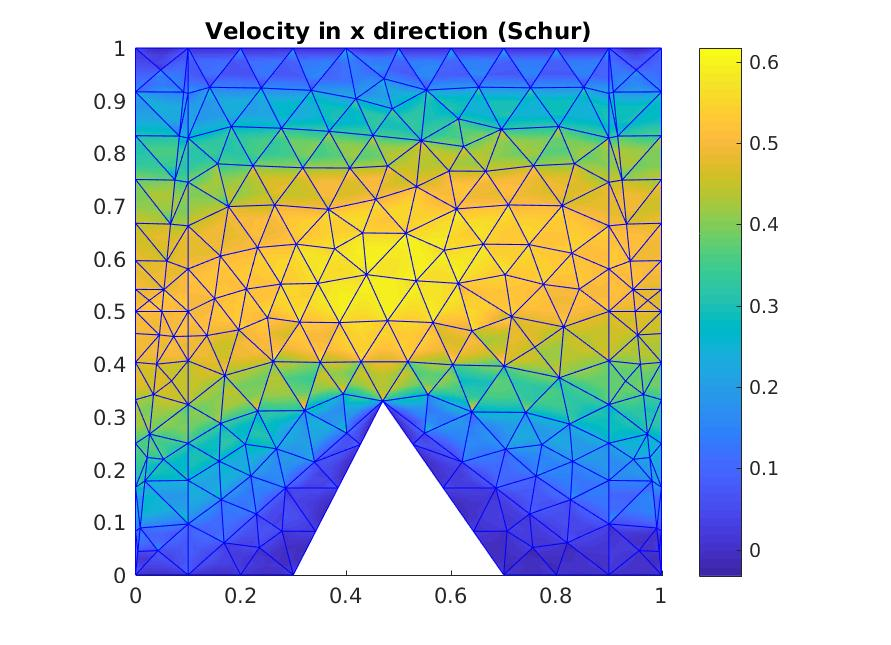
\includegraphics[width=\linewidth]{offline_velocity_1_at_47_33.jpg}
\caption{Velocity $x-$direction DGM solution} \label{vel_x_dg}
\end{subfigure}\hspace*{\fill}
\begin{subfigure}{0.31\textwidth}
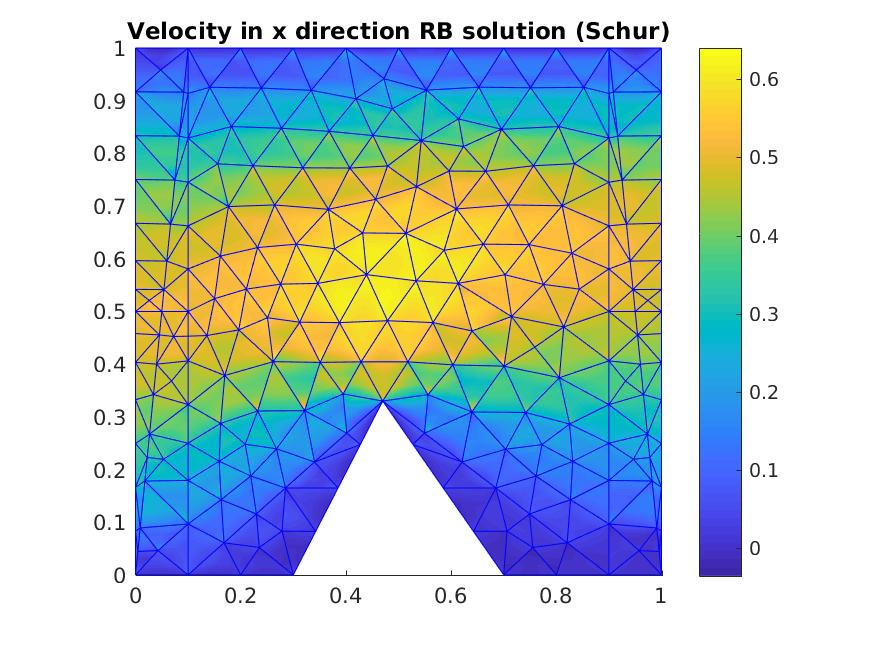
\includegraphics[width=\linewidth]{online_velocity_1_at_47_33.jpg}
\caption{Velocity $x-$direction RB solution} \label{vel_x_rb}
\end{subfigure}
\begin{subfigure}{0.31\textwidth}
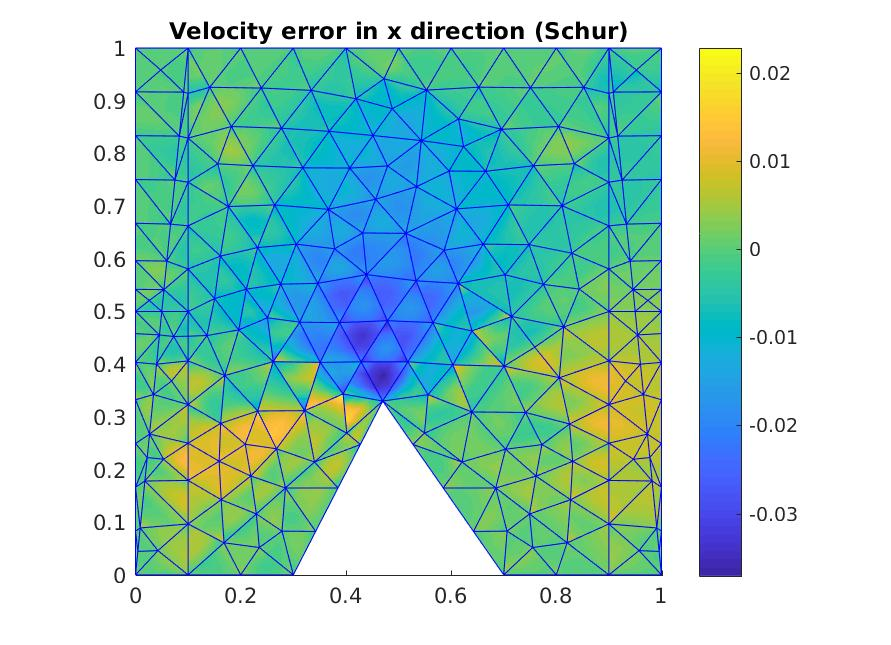
\includegraphics[width=\linewidth]{velocity_error_1_at_47_33.jpg}
\caption{$x-$component of Velocity absolute error $\overrightarrow{u}_h-\overrightarrow{u}_N$} \label{error_x_vel}
\end{subfigure}

\begin{subfigure}{0.31\textwidth}
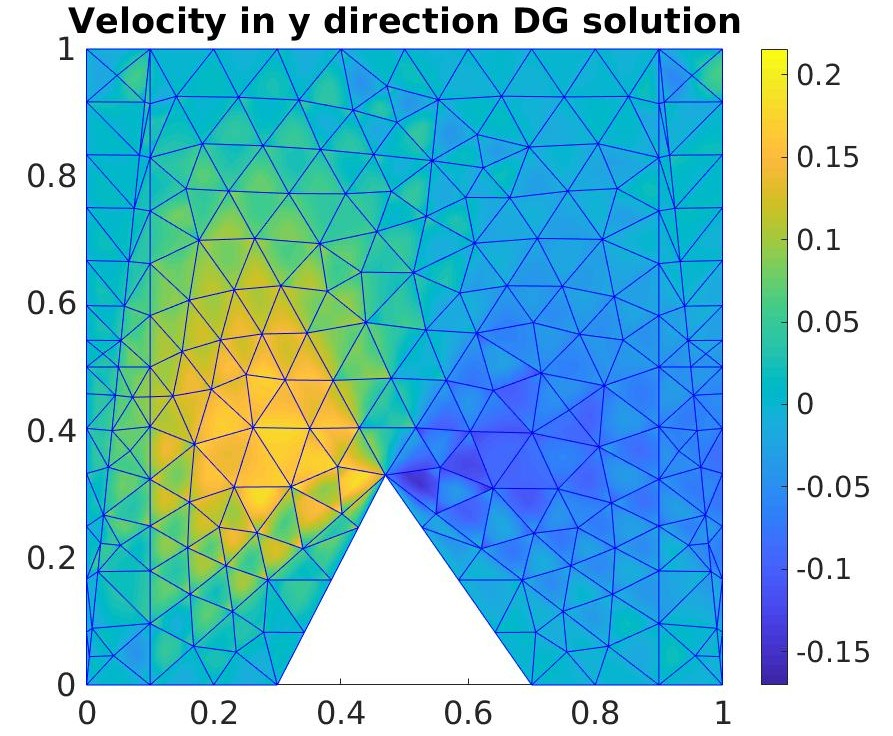
\includegraphics[width=\linewidth]{offline_velocity_2_at_47_33.jpg}
\caption{Velocity $y-$direction DGM solution} \label{vel_y_dg}
\end{subfigure}\hspace*{\fill}
\begin{subfigure}{0.31\textwidth}
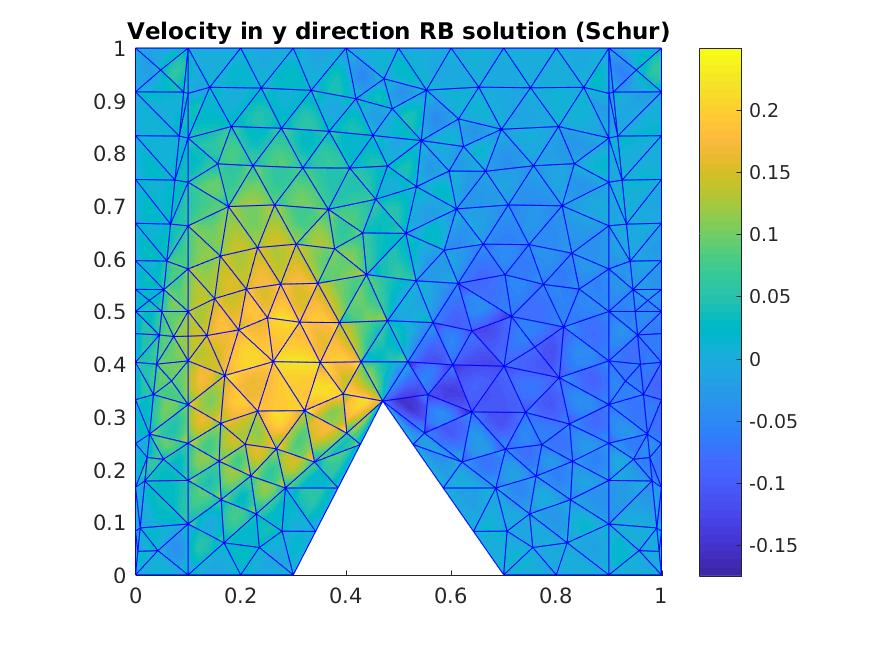
\includegraphics[width=\linewidth]{online_velocity_2_at_47_33.jpg}
\caption{Velocity $y-$direction RB solution} \label{vel_y_rb}
\end{subfigure}
\begin{subfigure}{0.31\textwidth}
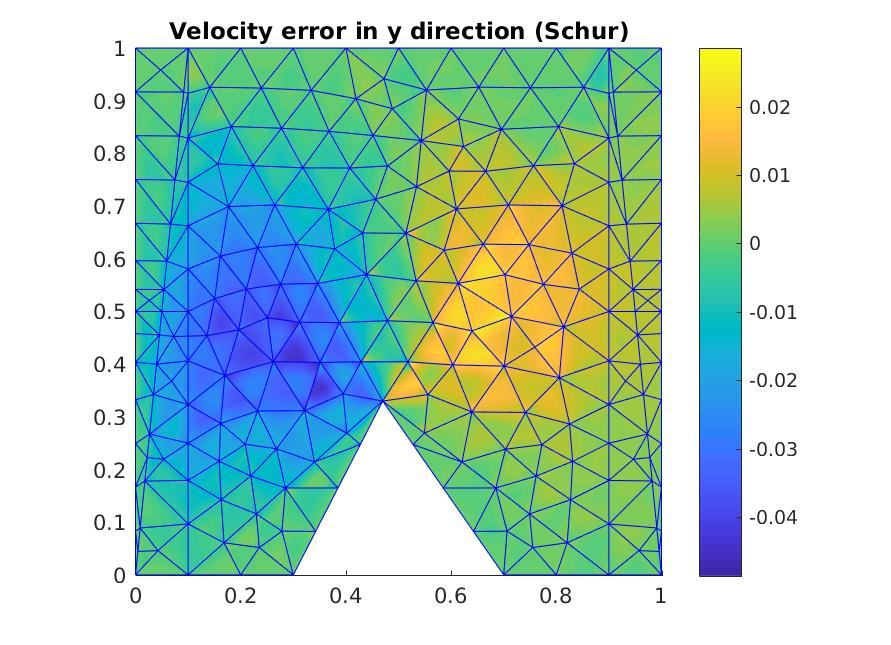
\includegraphics[width=\linewidth]{velocity_error_2_at_47_33.jpg}
\caption{$y-$component of Velocity absolute error $\overrightarrow{u}_h-\overrightarrow{u}_N$} \label{error_y_vel}
\end{subfigure}

\begin{subfigure}{0.31\textwidth}
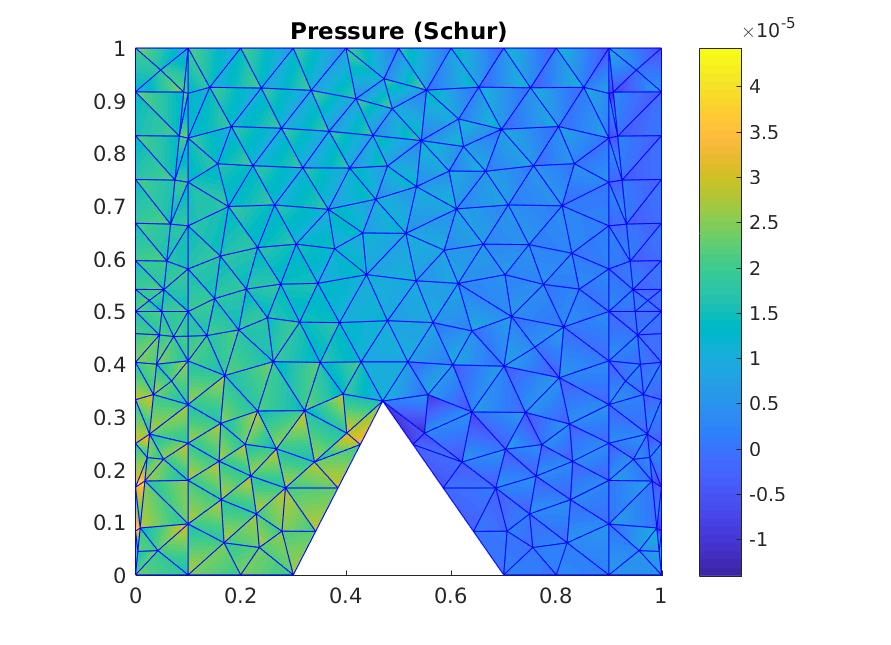
\includegraphics[width=\linewidth]{offline_pressure_at_47_33.jpg}
\caption{Pressure DGM solution} \label{pre_dg}
\end{subfigure}\hspace*{\fill}
\begin{subfigure}{0.31\textwidth}
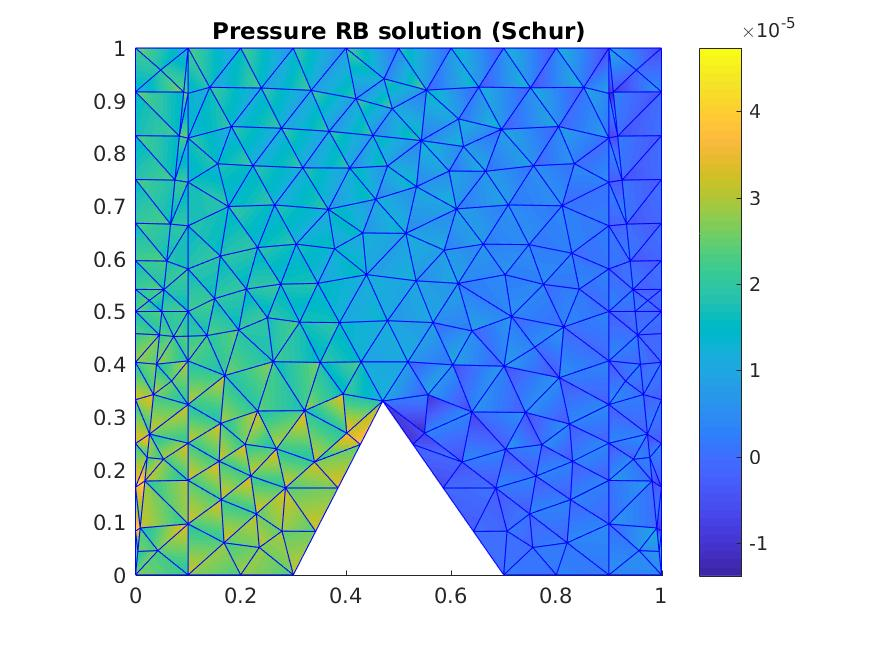
\includegraphics[width=\linewidth]{online_pressure_at_47_33.jpg}
\caption{Pressure RB solution} \label{pre_rb}
\end{subfigure}
\begin{subfigure}{0.31\textwidth}
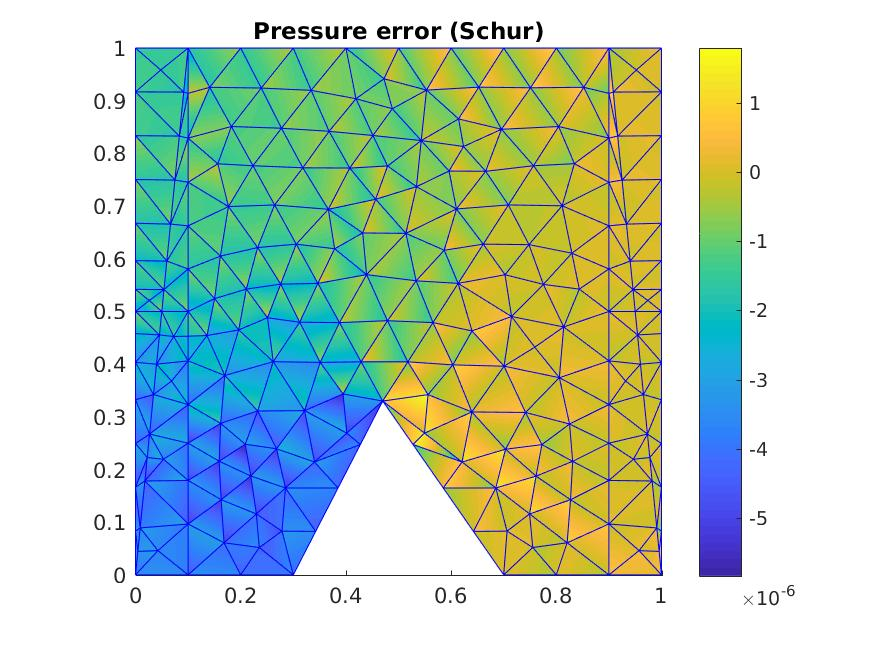
\includegraphics[width=\linewidth]{pressure_error_at_47_33.jpg}
\caption{Pressure absolute error $p_h-p_N$} \label{pre_error}
\end{subfigure}
\caption{DGM and RB solution $\mu = [\mu_x \ \mu_y] = [0.47 \ 0.33]$} 
\label{dg_rb_solution_47_33}
\end{figure}

\begin{figure}[H]
\begin{subfigure}{0.48\textwidth}
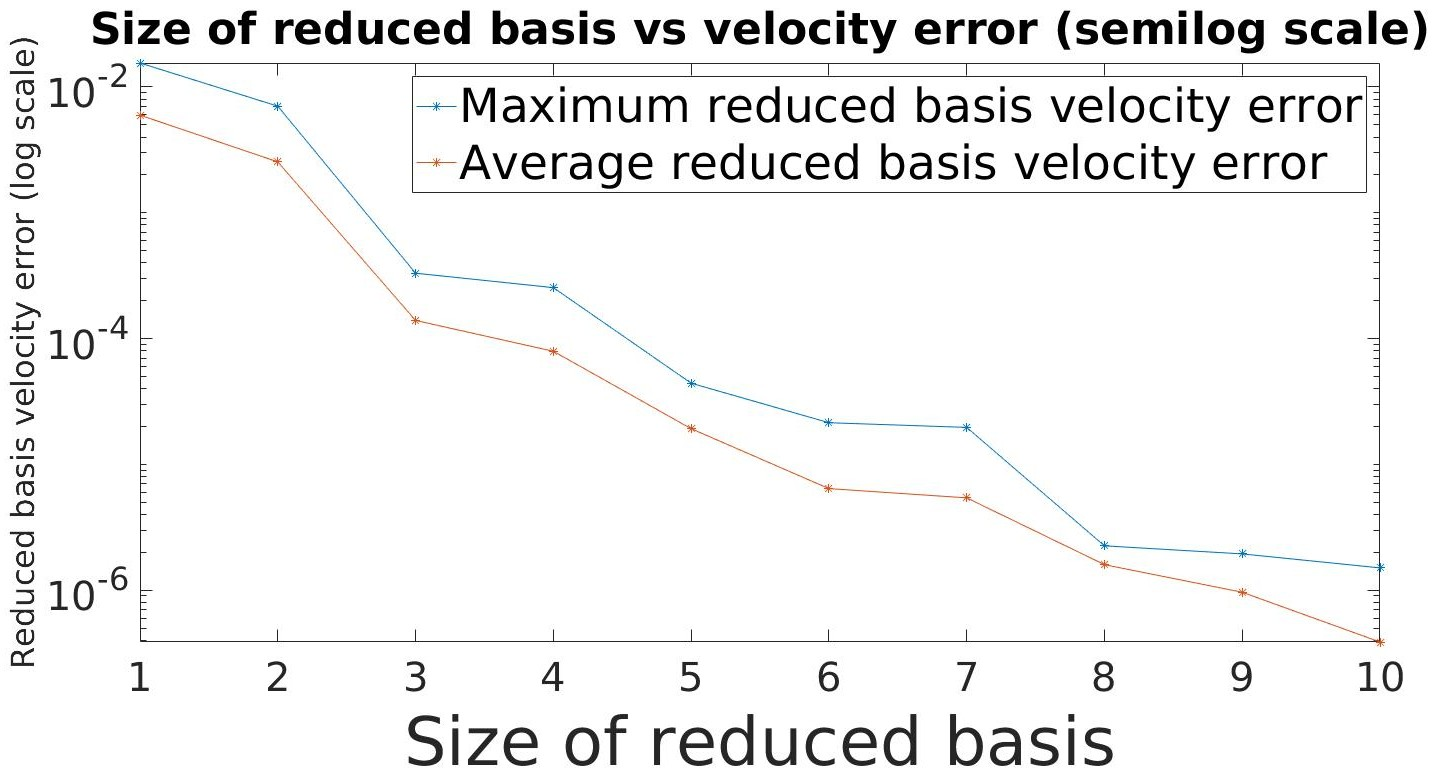
\includegraphics[width=\linewidth]{size_vs_reduced_basis_velocity_error_semilog.jpg}
\caption{Size of reduced basis space vs. Average relative error in velocity with inner product induced by $\bm{M}_v$} \label{error_vs_basis_velocity}
\end{subfigure}\hspace*{\fill}
\begin{subfigure}{0.48\textwidth}
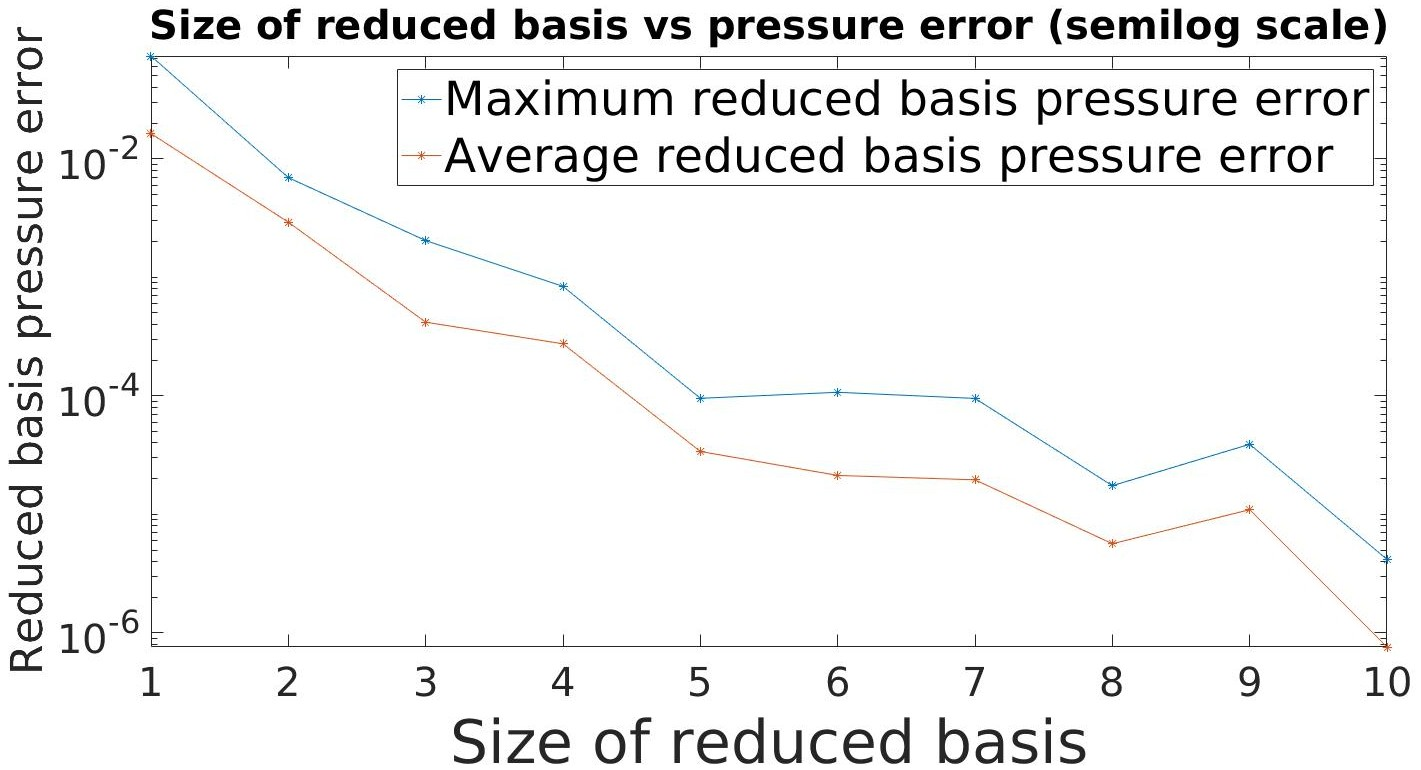
\includegraphics[width=\linewidth]{size_vs_reduced_basis_pressure_error_semilog.jpg}
\caption{Size of reduced basis space vs. Average relative error in pressure with inner product induced by $\bm{M}_p$} \label{error_vs_basis_pressure}
\end{subfigure}
  \caption{Size of reduced basis space vs Average relative error} 
\label{error_vs_basis}
\end{figure}

\begin{figure}[H]
\begin{subfigure}{0.31\textwidth}
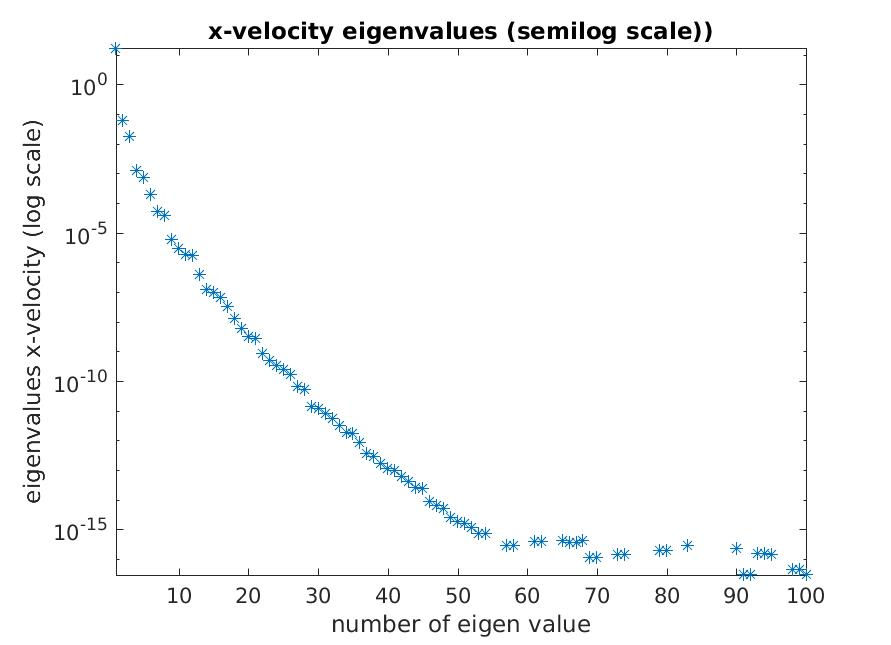
\includegraphics[width=\linewidth]{x_velocity_eigen_value_semilog.jpg}
\caption{$x-$Velocity eigenvalues (semilog scale)} \label{vel_x_ev}
\end{subfigure}\hspace*{\fill}
\begin{subfigure}{0.31\textwidth}
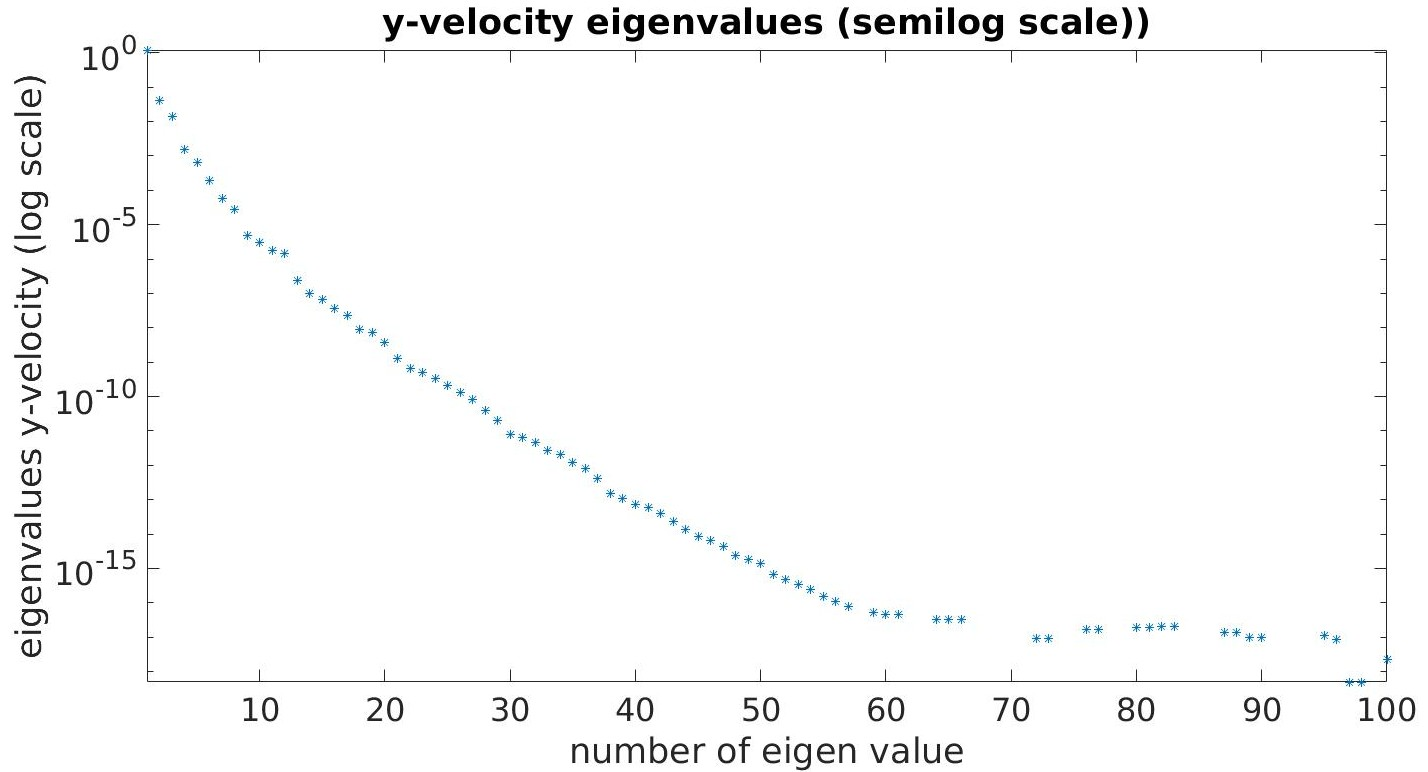
\includegraphics[width=\linewidth]{y_velocity_eigen_value_semilog.jpg}
\caption{$y-$Velocity eigenvalues (semilog scale)} \label{vel_y_ev}
\end{subfigure}
\begin{subfigure}{0.31\textwidth}
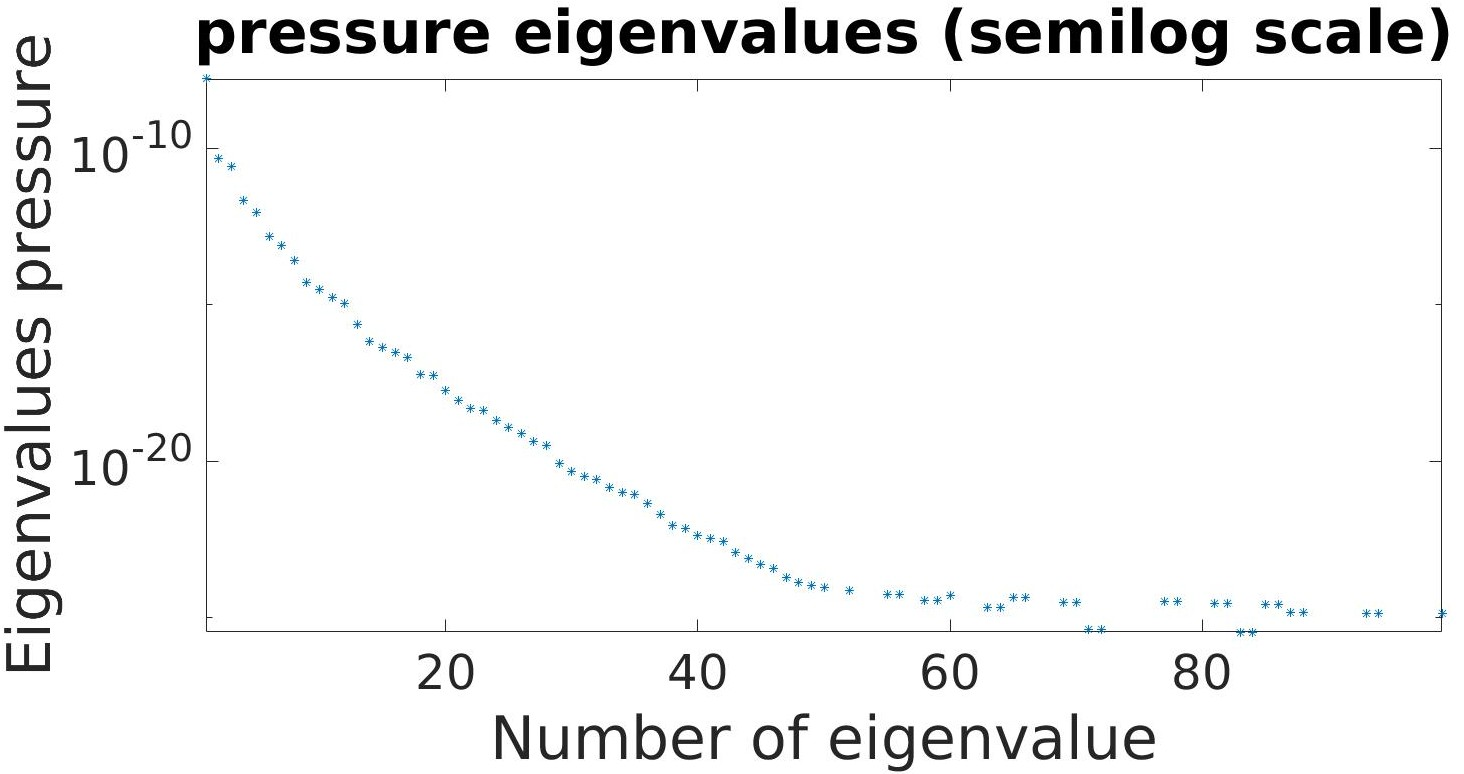
\includegraphics[width=\linewidth]{pressure_eigen_value_semilog.jpg}
\caption{Pressure eigenvalues (semilog scale)} \label{pressure_ev}
\end{subfigure}
\caption{Eigenvalue decay}\label{ev_decay}
\end{figure}

%\section{Concluding remarks}
%
%The potential of proper orthogonal decomposition as applied to geometrically parametrized discontinuous Galerkin formulation of Stokes equation was demonstrated. We expect this work to contribute towards further developments in the field of geometric parametrization and reduced basis method for the discontinuous Galerkin method.

\bibliographystyle{spbasic}
\bibliography{references}
%%%%%%%%%%%%%%%%%%%%% author.tex %%%%%%%%%%%%%%%%%%%%%%%%%%%%%%%%%%%
%
% sample root file for your "contribution" to a contributed volume
%
% Use this file as a template for your own input.
%
%%%%%%%%%%%%%%%% Springer %%%%%%%%%%%%%%%%%%%%%%%%%%%%%%%%%%


% RECOMMENDED %%%%%%%%%%%%%%%%%%%%%%%%%%%%%%%%%%%%%%%%%%%%%%%%%%%
\documentclass[graybox]{svmult}

% choose options for [] as required from the list
% in the Reference Guide

\usepackage{type1cm}        % activate if the above 3 fonts are
                            % not available on your system
%
\usepackage{makeidx}         % allows index generation
\usepackage{graphicx}        % standard LaTeX graphics tool
                             % when including figure files
\usepackage{multicol}        % used for the two-column index
\usepackage[bottom]{footmisc}% places footnotes at page bottom


\usepackage{newtxtext}       % 
\usepackage{newtxmath}       % selects Times Roman as basic font

\usepackage{url}

%%Nirav added
\newenvironment{spmatrix}[1]
 {\def\mysubscript{#1}\mathop\bgroup\begin{pmatrix}}
 {\end{pmatrix}\egroup_{\textstyle\mathstrut\mysubscript}}
\DeclareMathOperator{\Tr}{Tr}
\DeclareMathOperator{\spn}{span}
\usepackage{bm}
\usepackage{tikz}
\usepackage{wrapfig}
\usepackage[export]{adjustbox}
\usepackage{subcaption}
\usepackage{natbib}
\captionsetup{compatibility=false}
%%Nirav added over

% see the list of further useful packages
% in the Reference Guide

\makeindex             % used for the subject index
                       % please use the style svind.ist with
                       % your makeindex program

%%%%%%%%%%%%%%%%%%%%%%%%%%%%%%%%%%%%%%%%%%%%%%%%%%%%%%%%%%%%%%%%%%%%%%%%%%%%%%%%%%%%%%%%%

\begin{document}

\title{Discontinuous Galerkin model order reduction of geometrically parametrized Stokes flow}
% Use \titlerunning{Short Title} for an abbreviated version of
% your contribution title if the original one is too long
\author{Nirav Vasant Shah, Martin Hess and Gianluigi Rozza}
% Use \authorrunning{Short Title} for an abbreviated version of
% your contribution title if the original one is too long
\institute{Nirav Vasant Shah \at Scuola Internazionale Superiore di Studi Avanzati - via Bonomea, 265 - 34136 Trieste ITALY, \email{snirav@sissa.it}
\and Martin Hess \at Scuola Internazionale Superiore di Studi Avanzati - via Bonomea, 265 - 34136 Trieste ITALY \email{martin.hess@sissa.it}}
%
% Use the package "url.sty" to avoid
% problems with special characters
% used in your e-mail or web address
%
\maketitle

\abstract*{Each chapter should be preceded by an abstract (no more than 200 words) that summarizes the content. The abstract will appear \textit{online} at \url{www.SpringerLink.com} and be available with unrestricted access. This allows unregistered users to read the abstract as a teaser for the complete chapter.
Please use the 'starred' version of the \texttt{abstract} command for typesetting the text of the online abstracts (cf. source file of this chapter template \texttt{abstract}) and include them with the source files of your manuscript. Use the plain \texttt{abstract} command if the abstract is also to appear in the printed version of the book.}

\abstract{The present work focuses on geometrical parametrization and reduced order modeling of Stokes flow. We discuss the concept of geometric parametrization and its application along with importance of reduced order model technique.  The full order model is based on discontinuous Galerkin method interior penalty formulation. We introduce broken Sobolev spaces, relevant norms, jump and mean operator, weak formulation. The operators are transformed from fixed domain to parameter dependent domain by exploring affine parameter dependence. Proper orthogonal decomposition is applied to geometrically parametrized Stokes flow to obtain basis of function space for reduced order model. By using Galerkin projection the linear system is projected onto reduced space. During the process, offline-online decomposition is used to separate parameter independent and parameter independent operations. Finally the technique is applied to a test problem. The numerical outcomes presented include the experimental error analysis and measurement of online simulation time. \cite{psysoc-journal}\\
\textbf{Keywords:} Discontinuous Galerkin method, Stokes flow, Geometric parametrization, Proper orthogonal decomposition }

\section{Introduction}
\label{introduction}

The subject of mathematical applications in fluid mechanics starts with one of the variants of the Navier-Stokes equations, such as the Stokes equation. Almost all processes of fluid mechanics require considerations related to the Navier-Stokes equations. Navier-Stokes equation is non-linear, characterizing flow fluctuations. However, in case of laminar flow, i.e. when fluctuations are negligible, this linearized form of the Navier-Stokes equation is the Stokes equation.

Discontinuous Galerkin method (DGM) has found traction as numerical method for elliptic problems \textbf{pereire reference} as well as hyperbolic problems \textbf{Book on compressible flow reference}. This is due to its several advantages over Finite Element Method (FEM) and Finite Volume Method (FVM). In fact, DGM is considered as combination of FEM and FVM. DGM uses polynomial approximation of suitable degree providing higher accuracy as well as allows discontinuity at the interface, by the concept of numerical flux, allowing greater flexibility. This fact makes DGM naturally attractive to problems, such as shock capturing, due to presence of steep gradients or discontinuities. Additionally, since the Dirichlet conditions are applied as boundary penalty, it avoids necessity to work with subspace of Sobolev space such as in case of FEM. Several variants of DGM exist based on computational advantages such as sparsity pattern or extension of computational stencil, complexity of numerical implementation etc.

Geometric parametrization has emerged as important application of Parametric Partial Differential Equations (PPDEs) and as alternative to shape optimization. The concept of geometric parametrization allows to transfer operator evaluated on one geometric domain to another geometric domain efficiently. For linear equations, this means exploiting affine parameter dependence as will be shown in later section. Model Order Reduction (MOR) on the other hand allows reducing the size of the system to be solved and working with the smaller system containing only dominant components and discarding the non-dominant components. It is pertinent to mention that identifying "dominant" components is critical to the success of model order reduction strategy. Optimization of engineering components using geometric parametrization combined with MOR for PPDEs has given quite useful results in the fields such as mechanical, naval and aeronautic designs. Also, the  faster computations obtained by MOR has helped in many query context, real time computation and quick transfer of computational results to industrial problems.

In the present work, we first introduce notion of parametrization characterizing geometry of the domain under consideration. We subsequently introduce Discontinuous Galerkin Interior Penalty Method (DG-IPM) for stokes flow. We then explain exploiting affine parameter dependence and its application in the context of offline-online decomposition. We then apply Proper Orthogonal Decomposition (POD) for constructing reduced basis space and apply Galerkin projection to project the system of equations on the space constructed by POD. Finally we present a test problem to demonstrate the introduced method and numerical result.

\section{Geometric parametrization}\label{geometric_parametrization_section}

Consider domain $\Omega = \Omega(\mu) \in \mathbb{R}^d$ as open bounded domain. The parameter set $\mu \in \mathbb{P}$, where $\mathbb{P}$ is parameter space, completely characterizes the domain. Also, consider a parameter set $\bar{\mu} \in \mathbb{P}$, as the known parameter set and $\Omega(\bar{\mu})$ as the reference domain, whose configuration is completely known. The mapping $\bm{F}(\cdot,\mu) : \Omega(\bar{\mu}) \rightarrow \Omega(\mu)$ links reference domain and parametrized domain. Divide the domain $\Omega(\mu)$ into $n_{su}$ subdomains such that $\Omega(\mu) = \bigcup\limits_{i=1}^{n_{su}} \Omega_i(\mu) \ , \ \Omega_i(\mu) \bigcap \Omega_j(\mu) = \emptyset \ , \ \text{for} \ i \neq j$. The boundary of $\Omega(\mu)$, that is $\partial \Omega(\mu)$ is divided into Neumann boundary $\Gamma_N(\mu)$ and Dirichlet boundary $\Gamma_D(\mu)$ i.e. $\partial \Omega(\mu) = \Gamma_N(\mu) \cup \Gamma_D(\mu)$.

In the case of affine transformation, $\bm{F}$ is of the form,
\begin{gather}\label{affine_F}
x = \bm{F}(\hat{x},\mu) = \bm{G}_F(\mu)\hat{x} + c_F(\mu) \ ; \forall x \in \Omega \ , \ \hat{x} \in \Omega(\bar{\mu}) \ .
\end{gather}

The inverse map $\bm{T}$ is expressed in the form,
\begin{gather}\label{affine_T}
\hat{x} = \bm{T}(x,\mu) = \bm{G}_T(\mu)x + c_T(\mu) \ ; \forall x \in \Omega \ , \ \hat{x} \in \Omega(\bar{\mu}) \ .
\end{gather}

\section{Discontinuous Galerkin formulation}
\label{DG_formulation}

Each subdomain is divided into $N_{el}$ number of triangular elements $\tau_k$ such that $\Omega = \bigcup\limits_{k=1}^{N_{el}} \tau_k$. The triangulation $\mathcal{T}$ is the set of all triangular elements i.e. $\mathcal{T} = \lbrace \tau_k \rbrace_{k=1}^{N_{el}}$. The internal boundary $\Gamma = \lbrace \bigcup\limits_{k=1}^{N_{el} \partial \tau_k \rbrace} \backslash \partial \Omega$. The vertices of triangle ${\tau_k}_{k=1}^{N_{el}}$ are called nodes. $\overrightarrow{n}$ is the outward pointing normal to an edge of element.

The Stokes's equation in strong form can be stated as,
\begin{gather}\label{stokes_strong_form}
-\nu \Delta \overrightarrow{u} + \nabla p = \overrightarrow{f} \ , \ \text{in } \Omega \ , \\
\nabla \cdot \overrightarrow{u} = 0 \ , \ \text{in} \ \Omega \ , \\
\overrightarrow{u} = \overrightarrow{u}_D \ , \ \text{on } \Gamma_D \ , \\
-p \overrightarrow{n} + \nu \overrightarrow{n} \cdot \nabla \overrightarrow{u} = \overrightarrow{t} \ , \ \text{on} \ \Gamma_N \ .
\end{gather}

The velocity vector field $\overrightarrow{u}$ and pressure scalar field $p$ are the unknowns. $\nu$ is the material property known as kinematic viscosity. Vector $\overrightarrow{f}$ is external force term or source term. $\overrightarrow{u}_D$ is the Dirichlet velocity and $\overrightarrow{t}$ is the Neumann value.

Before introducing weak form let us introduce broken Sobolev spaces for variables.

The space for velocity is 
\begin{equation} \label{velocity_test}
\mathbb{V} = \lbrace \overrightarrow{\phi} \in (L^2(\Omega))^d | \ \overrightarrow{\phi} \in (P^D(\tau_k))^d \ , \ \tau_k \in \mathcal{T} \rbrace \ .
\end{equation}
The space for pressure is 
\begin{equation} \label{pressure_test}
\mathbb{Q} = \lbrace \psi \in (L^2(\Omega)) | \ \psi \in (P^{D-1}(\tau_k)) \ , \ \tau_k \in \mathcal{T} \rbrace \ .
\end{equation}
Here, $P^D(\tau_k)$ denotes space of polynomials of degree at most $D \geq 2$ over $\tau_k$.

The velocity $\overrightarrow{u}(x)$ and pressure $p(x)$ at any point $x \in \Omega$ is given by,
\begin{equation}\label{velocity_pressure_coefficients}
\overrightarrow{u}(x) = \sum\limits_{i=1}^{\overrightarrow{u}_{ndofs}} \overrightarrow{\phi}_i \hat{u}_i \ , \
p(x) = \sum\limits_{i=1}^{p_{ndofs}} \psi_i \hat{p}_i \ ,
\end{equation}
where $\hat{u}_i$'s and $\hat{p}_i$'s are coefficients of velocity basis functions and pressure basis functions respectively. 

\begin{figure}
\centering
\sidecaption[t]
\begin{tikzpicture}
\draw (0,0) node[anchor=north]{${}$}
  -- (4,0) node[anchor=north]{${}$}
  -- (0,4) node[anchor=south]{${}$}
  -- cycle;
\draw (4,4) node[anchor=north]{${}$}
  -- (4,0) node[anchor=north]{${}$}
  -- (0,4) node[anchor=south]{${}$}
  -- cycle;
\draw[->] (2,2)--(2.5,2.5)node[label={[xshift=0.4cm, yshift=-0.7cm]${\overrightarrow{n}^-}$}]{};
\draw[->] (2,2)--(1.5,1.5)node[label={[xshift=0cm, yshift=0cm]${\overrightarrow{n}^+}$}]{};
\node at (1,1){$\tau_{k}^-$};
\node at (3,3){$\tau_{k}^+$};
\node at (1.7,3){$\overrightarrow{\phi}^+,\psi^+$};
\node at (2.3,1){$\overrightarrow{\phi}^-,\psi^-$};
\end{tikzpicture}
\caption{Definition of jump and mean operator. \newline The superscript $+$ refers to quantity in the element itself and the superscript $-$ refers to quantity in the neighboring element}
\label{fig:Self_neighbour}
\end{figure}

In the subsequent sections $\left( \cdot \right),\left( \cdot \right)_{\Gamma_D},\left( \cdot \right)_{\Gamma_N},\left( \cdot \right)_{\Gamma}$ represent the $L^2$ scalar product over $\Omega,\Gamma_D,\Gamma_N,\Gamma$ respectively. The jump operator $\left[ \cdot \right]$ and the average operator $\lbrace \cdot \rbrace$ are are important concepts in DGM formulation and are required to approximate the numerical flux (Figure \ref{fig:Self_neighbour}).

The presence of normal vector $\overrightarrow{n}$ in jump and average operator introduced below allows symmetric formulation and also ensures that jump of a vector is vector and jump of a scalar is scalar.

\begin{itemize}
\item For vector quantity $\overrightarrow{\phi}$:
\begin{itemize}
\item Jump operator: 
$\left[\overrightarrow{\phi} \cdot \overrightarrow{n}\right] = \overrightarrow{\phi}^+ \cdot \overrightarrow{n}^+ + \overrightarrow{\phi}^- \cdot \overrightarrow{n}^-$ on $\Gamma$, $\left[\overrightarrow{\phi} \cdot \overrightarrow{n}\right] = \overrightarrow{\phi} \cdot \overrightarrow{n}$ on $\partial \Omega$.
\item Average operator:
$\lbrace \overrightarrow{\phi} \rbrace = \frac{\overrightarrow{\phi}^+ + \overrightarrow{\phi}^-}{2}$ on $\Gamma$, $\lbrace \overrightarrow{\phi} \rbrace = \overrightarrow{\phi}$ on $\partial \Omega$.
\end{itemize}
\item For scalar quantity $\psi$:
\begin{itemize}
\item Jump operator:
$\left[\psi \overrightarrow{n} \right] = \psi^+ \overrightarrow{n}^+ + \psi^- \overrightarrow{n}^-$ on $\Gamma$, $\left[\psi \overrightarrow{n} \right] = \psi \overrightarrow{n}$ on $\partial \Omega$.
\item Average operator:
$\lbrace \psi \rbrace = \frac{\psi^+ + \psi^-}{2}$ on $\Gamma$, $\lbrace \psi \rbrace = \psi$ on $\partial \Omega$. 
\end{itemize}
\end{itemize}

The weak form of Stokes equation is as follow,
\begin{gather}\label{stokes_weak_ch3}
a_{IP}(\overrightarrow{u},\overrightarrow{\phi}) + b(\overrightarrow{\phi},p) + \left( \lbrace p \rbrace,[\overrightarrow{n} \cdot \overrightarrow{\phi}] \right)_{\Gamma \cup \Gamma_D} = l_{IP}(\overrightarrow{\phi}) \ , \\
a_{IP}(\overrightarrow{u},\overrightarrow{\phi}) = \left( \nabla \overrightarrow{u}, \nabla \overrightarrow{\phi} \right) + C_{11} \left( [\overrightarrow{u}],[\overrightarrow{\phi}] \right)_{\Gamma \cup \Gamma_D} - \nu \left( \lbrace \nabla \overrightarrow{u}\rbrace ,[\overrightarrow{n} \otimes \overrightarrow{\phi}] \right)_{\Gamma \cup \Gamma_D} - \nu \left( [\overrightarrow{n} \otimes \overrightarrow{u}], \lbrace \nabla \overrightarrow{\phi} \rbrace \right)_{\Gamma \cup \Gamma_D} \ , \\
b(\phi,\psi) = -\int_{\mathcal{T}} \psi \nabla \cdot \overrightarrow{\phi} \ , \\
l_{IP}(\overrightarrow{\phi}) = \left( \overrightarrow{f},\overrightarrow{\phi} \right) + \left( \overrightarrow{t},\overrightarrow{\phi} \right)_{\Gamma_N} + C_{11} \left(\overrightarrow{u}_D,\overrightarrow{\phi}\right)_{\Gamma_D} - \left( \overrightarrow{n} \otimes \overrightarrow{u}_D, \nu \nabla \overrightarrow{\phi} \right)_{\Gamma_D} \ .
\end{gather}

The penalty parameter $C_{11}>0$ in $a_{IP}(\overrightarrow{u},\overrightarrow{\phi})$ is an empirical constant to be kept large enough to maintain coercivity of bilinear form.

The weak for of continuity equation is as follow,
\begin{equation}\label{contiuity_weak_ch3}
\begin{split}
b(\overrightarrow{u},\psi) + ({\psi},[\overrightarrow{n} \cdot \overrightarrow{u}])_{\Gamma \cup \Gamma_D} = (\psi,\overrightarrow{n} \cdot \overrightarrow{u}_D)_{\Gamma_D} \ .
\end{split}
\end{equation}

In discrete form system of equations can be written as, 
\begin{equation} \label{Stokes_matrix_ch3}
\begin{spmatrix}{\textrm{Stiffness matrix}}
    \bm{A} & \bm{B} \\
    \bm{B}^T & 0
\end{spmatrix}
\begin{spmatrix}{\textrm{Solution vector}}
    U \\
    P
\end{spmatrix}
=
\begin{spmatrix}{\textrm{Right hand side (Known)}}
    F_1  \\
    F_2
\end{spmatrix}
\textrm{.}
\end{equation}

Here, $\bm{A}_{ij} = a_{IP} (\overrightarrow{\phi}_i,\overrightarrow{\phi}_j)$, $\bm{B}_{ij} = b(\overrightarrow{\phi}_i,\psi_j) + \left( \lbrace \psi_j \rbrace , [n \cdot \phi_i]\right)_{\Gamma \cup \Gamma_D}$, $F_1 = l_{IP}(\overrightarrow{\phi}_i)$ and $F_2 = \left( \psi_j,\overrightarrow{n} \cdot \overrightarrow{u}_D \right)_{\Gamma_D}$. The column vectors $U$ and $P$ are coefficients $\hat{u}$'s and $\hat{p}$'s from equation \eqref{velocity_pressure_coefficients}.

\section{Affine expansion}

We evaluate and solve the Stokes equation weak formulation on reference domain $\Omega{\bar{\mu}}$. Given a parameter set $\mu \neq \bar{\mu}$ we need to evaluate the linear systems of equation \eqref{Stokes_matrix_ch3} on new domain $\Omega(\mu)$. To accomplish this we use affine expansion using linear nature of equation and diving $\Omega(\bar{\mu})$ into triangular subdomains $\Omega_i(\bar{\mu}) \ , \ i = \lbrace 1,2,\ldots,n_{su} \rbrace$ as explained earlier in the section geometric parametrization [Section \ref{geometric_parametrization_section}]. The affine expansion of operators is essentially change of variable and has been explained in literatures such as \textbf{ADD affine expansion literature}. However it is pertinent to mention two expansions as specific to DGM formulation will be mentioned here as below.

\begin{itemize}
\item In order to transfer the terms containing jump and average operator following approach is used in present analysis.
\begin{equation*}\label{jump_average_term_split}
\begin{split}
\left(\lbrace \nabla \overrightarrow{\phi} \rbrace , \left[ \overrightarrow{n} \otimes \overrightarrow{\phi}  \right]  \right) = \left( \nabla \overrightarrow{\phi}^+ , \overrightarrow{n}^+ \otimes \overrightarrow{\phi}^+ \right) + \left( \nabla \overrightarrow{\phi}^+ , \overrightarrow{n}^- \otimes \overrightarrow{\phi}^- \right) + \\ 
\left( \nabla \overrightarrow{\phi}^- , \overrightarrow{n}^+ \otimes \overrightarrow{\phi}^+ \right) + \left( \nabla \overrightarrow{\phi}^- , \overrightarrow{n}^- \otimes \overrightarrow{\phi}^- \right) \ .
\end{split}
\end{equation*}
Each term on right hand side of equation \eqref{jump_average_term_split} can now be transformed using affine map.

\item The coercivity term $C_{11}\left( [\overrightarrow{\phi}],[\overrightarrow{u}] \right)_{\Gamma \cup \Gamma_D}$ is not transformed but used as evaluated on reference domain $\Omega(\bar{\mu})$. The affine transformation is given by,
\begin{equation*}
\begin{split}
C_{11}\left( [\overrightarrow{\phi}(\hat{x}),\overrightarrow{u}(\hat{x})] \right)_{\Gamma(\mu) \cup \Gamma_D(\mu)} = C_{11} \alpha \left( [\overrightarrow{\phi}(\bm{F}(\hat{x})),\overrightarrow{u}(\bm{F}(\hat{x}))] \right)_{\Gamma(\bar{\mu}) \cup \Gamma_D(\bar{\mu})} \ , \\
\alpha = \frac{meas\left( \Gamma(\mu) \cup \Gamma_D(\mu)\right)}{meas\left( \Gamma(\bar{\mu}) \cup \Gamma_D(\bar{\mu})\right)} \ , \ \hat{x} \in \Omega(\bar{\mu}) \ , \ x \in \Omega(\mu) \ .
\end{split}
\end{equation*}

Since, $C_{11}$ is empirical coefficient replacing $C_{11} \alpha$ with $C_{11}$ will not change the formulation as long as coercivity of $a_{IP}$ over parameter space $\mathbb{P}$ is maintained. In the present analysis, $C_{11}$ is not calculated exactly but only order of magnitude required for $C_{11}$ is estimated and $C_{11}$ is kept one magnitude larger as safeguard against round-off errors. As long as the domain $\Omega(\mu)$ is not deformed much compared to its reference configuration $\Omega(\bar{\mu})$, $C_{11}$ and $C_{11}\alpha$ will have the same order of magnitude. However, regardless of this fact, large deformations are not favorable as it will lead to bad mesh quality and in turn, will lead to poor DGM-approximation.
\end{itemize}

\section{Reduced basis method}

\subsection{Snapshot proper orthogonal decomposition}\label{POD_section}

We present now snapshot proper orthogonal decomposition method. Here, ``snapshot" means solution calculated by discontinuous Galerkin method. We calculate solution based on $\mu_n, n \in \lbrace 1,....,n_s \rbrace$ i.e. $n_s$ snapshots are generated. We also introduce inner product matrices $\bm{M}_v \in \mathbb{R}^{\overrightarrow{u}_{ndofs} \times \overrightarrow{u}_{ndofs}}$ and $\bm{M}_p \in \mathbb{R}^{p_{ndofs} \times p_{ndofs}}$.

\begin{gather*}
\bm{M}_v = \int_{\Omega} \overrightarrow{\phi}_i \cdot \overrightarrow{\phi}_j + \sum_{k=1}^{N_{el}} \int_{\tau_k} \nabla \overrightarrow{\phi}_i : \nabla \overrightarrow{\phi}_j \ , \ i,j = 1, \ldots, \overrightarrow{u}_{ndofs} \ , \\
\bm{M}_p = \int_{\Omega} \psi_i \psi_j \ , \ i,j = 1, \ldots, p_{ndofs} \ .
\end{gather*}

We also introduce matrices storing velocity snapshots $\bm{S}_v$ and storing pressure snapshots $\bm{S}_p$. We discuss the method only for velocity snapshots. The method is similar for pressure snapshots. We note the size of matrices, useful for matrix operations presented hereafter.

\begin{gather*}
\bm{S}_v \in \mathbb{R}^{\overrightarrow{u}_{ndofs} \times n_s} \ , \ \bm{S}_p \in \mathbb{R}^{p_{ndofs} \times n_s} \ , \\
\bm{M}_v \in \mathbb{R}^{\overrightarrow{u}_{ndofs} \times \overrightarrow{u}_{ndofs}} \ ,\ \bm{M}_p \in \mathbb{R}^{p_{ndofs} \times p_{ndofs}} \ .
\end{gather*}

\subsection{Spectral decomposition of snapshots}\label{spectral_decomposition_section}

We denote the dimension of reduced basis as $N$ and assert that $N << n_s$. We now perform the spectral decomposition of $\bm{S}_v^T \bm{M}_v \bm{S}_v$,

\begin{equation}\label{snapshot_eigen_value}
\bm{S}_v^T \bm{M}_v \bm{S}_v = \bm{V} \bm{\Theta} \bm{V}^T \ .
\end{equation}

The columns of $V$ are eigenvectors and $\Theta$ has eigenvalues $\theta_i \ , \ 1 \leq i \leq n_s$ such that,
\begin{equation}
\Theta_{ij} = \theta_i \delta_{ij} \ .
\end{equation}

We also note that $\theta_i > 0$ and $\theta_1 \geq \theta_2 \geq ... \geq \theta_{n_s}$ i.e. the eigenvalues are in sorted order. We form the reduced basis by linear combination of the snapshot vector,
\begin{equation}\label{linear_combination_snapshots}
\bm{B}_v = \bm{S}_v \bm{A} \ , \ \bm{A} \in \mathbb{R}^{n_s \times N} \ .
\end{equation}
the reduced basis for velocity basis function $\overrightarrow{\phi}_N$ is formed by,
\begin{equation}
\overrightarrow{\phi}_N = \overrightarrow{\phi}^T \bm{B}_v \ .
\end{equation}

Considering orthonormality of reduced basis $\overrightarrow{\phi}_N$ with respect to inner product induced by $\bm{M}_v$, from equation \eqref{snapshot_eigen_value},
\begin{equation}
<\overrightarrow{\phi}_N,\overrightarrow{\phi}_N>_{\bm{M}_v} = \bm{B}_v^T \bm{M}_v \bm{B}_v = I \ .
\end{equation}
From equation \eqref{linear_combination_snapshots}, we express matrix $\bm{A}$ as,
\begin{equation}
\bm{A} = \bm{V} \bm{\Theta}^{-\frac{1}{2}} \bm{R} \ , \ \bm{R} = [\bm{I}_{N \times N} ; \bm{0}_{(N-n_s \times N)}] \ \text{and accordingly} \ \bm{B}_v = \bm{S}_v \bm{V} \bm{\Theta}^{-\frac{1}{2}} \bm{R} \ .
\end{equation}
The columns of $\bm{B}_v$ now represent the basis functions for reduced space for velocity. Due to round-off errors, these basis functions may not be of unit magnitude and it is necessary to normalize the basis functions.

The reduced basis space $\bm{B}_p$ can be generated in similar manner using pressure snapshots $\bm{S}_p$ and inner product matrix $\bm{M}_p$.

\subsection{Galerkin reduced basis formulation}\label{Galerkin_section}

We now present the reduced bilinear form as,

\begin{equation} \label{stokes_equation_parameter}
a(u_N,\phi_N;\mu) + b(p_N,\phi_N;\mu) = f_1(\phi_N,\mu) \textrm{,}
\end{equation}

\begin{equation} \label{continuity_equation_parameter}
b(u_N,\psi_N;\mu) = f_2(\psi_N,\mu) \textrm{.}
\end{equation}

In discrete form, we form reduced equation as,

\begin{equation} \label{Stokes_matrix_reduced}
\begin{spmatrix}{\tilde{K}}
    \bm{B}_v^T \bm{A}(\mu) \bm{B}_v & \bm{B}_v^T \bm{B}(\mu) \bm{B}_v \\
    \bm{B}_p^T \bm{B}(\mu)^T \bm{B}_v & \bm{0}
\end{spmatrix}
\begin{spmatrix}{\zeta}
    U_N \\
    P_N
\end{spmatrix}
=
\begin{spmatrix}{\tilde{F}}
    \bm{B}_v^T F_1(\mu)  \\
    \bm{B}_p^T F_2(\mu)
\end{spmatrix} \ ,
\end{equation}
and accordingly we solve following variational form for reduced degrees of freedom $\zeta$,
\begin{equation}
\tilde{\bm{K}} \zeta = \tilde{F} \ ,
\end{equation}
and calculate reduced solutions $\overrightarrow{u}_N$ and $p_N$ as,
\begin{equation}
\overrightarrow{u}_N = \bm{B}_v U_N \ , \ p_N = \bm{B}_p P_N
\end{equation}

\section{Offline-online procedure}

The offline-online procedure is used to separate computationally intensive parameter independent offline procedure and faster parameter dependent online procedure \textbf{cite CRBM}. During the offline phase $n_s$ snapshots are computed and reduced basis spaces $\bm{B}_v$ and $\bm{B}_p$ are created. The offline procedure is outlined in section \ref{POD_section} and section \ref{spectral_decomposition_section}. During the online phase the systems of equations are projected on reduced space using Galerkin projection, the smaller systems of equation obtained by Galerkin projection is solved and the reduced basis solution is computed as outlined in section \ref{Galerkin_section}. The parameter dependent matrices in equation \eqref{Stokes_matrix_reduced} are evaluated by using affine decomposition.

\section{Numerical example}

We perform the POD-Galerkin method as mentioned in section \ref{POD_section} - section \ref{Galerkin_section}. The reference domain $\Omega{\bar{\mu}}$ is the unit square domain with triangle with vertices $(0.3,0),(0.5,0.3),(0.7,0)$ as obstacle. The geometric parameters are coordinates of tip of the obstacle i.e. $\bar{\mu} = (0.5,0.3)$. The boundary ${x=0}$ is Dirichlet boundary with inflow velocity at point $(0,y)$ as $u = (y(1-y), 0)$. The boundary ${x = 1}$ is a Neumann boundary with zero Neumann value i.e. $t = (0, 0)$. Other boundaries are Dirichlet boundary with no slip condition. The source term is $f = (0,0)$.

The training set was generated by random generation of $100$ parameters between the interval $[0.4,0.6] \times [0.4,0.6]$. The test set contained $10$ random parameters between the interval $[0.4,0.6] \times [0.4,0.6]$. For velocity basis function polynomial of degree $P^D = 2$ and for pressure basis function polynomial of degree $P^{D-1} = 1$ was used. The number of velocity degrees of freedom and pressure degrees of freedom were $\overrightarrow{u}_{ndofs} = 4704$ and $p_{ndofs} = 1176$ respectively.

Figure \ref{dg_rb_solution_47_33} shows solution computed by DGM and POD at parameter value $(0.47,33)$. Figure \ref{error_vs_basis} shows error vs size of reduced basis space. As can be seen the error drops with increasing size of basis function, however, this has to be at affordable cost of increased online simulation time (Figure \ref{basis_vs_time}).

\begin{figure}%[t!] % "[t!]" placement specifier just for this example
\begin{subfigure}{0.31\textwidth}
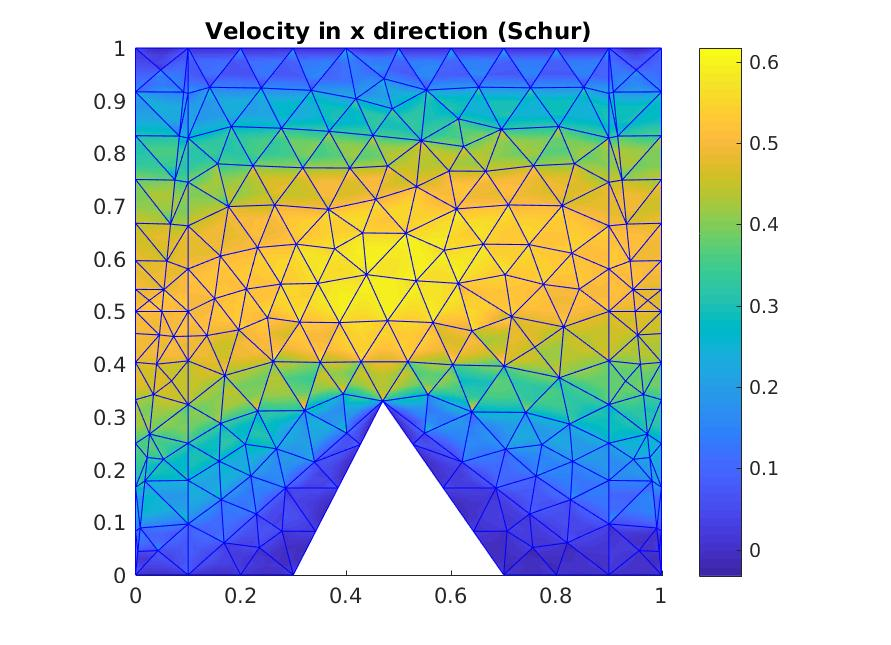
\includegraphics[width=\linewidth]{offline_velocity_1_at_47_33.jpg}
\caption{Velocity $x-$direction DG solution} \label{vel_x_dg}
\end{subfigure}\hspace*{\fill}
\begin{subfigure}{0.31\textwidth}
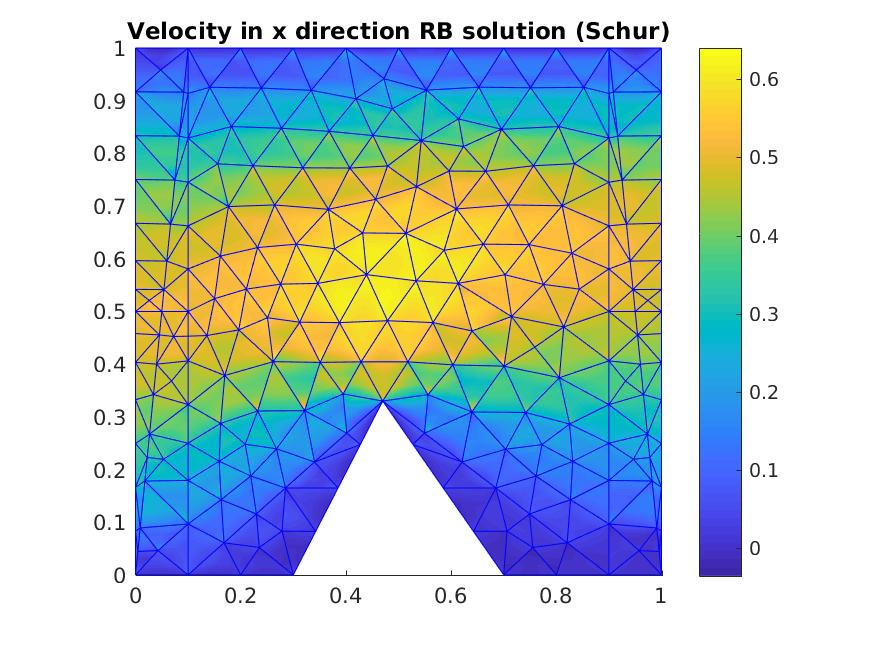
\includegraphics[width=\linewidth]{online_velocity_1_at_47_33.jpg}
\caption{Velocity $x-$direction RB solution} \label{vel_x_rb}
\end{subfigure}
\begin{subfigure}{0.31\textwidth}
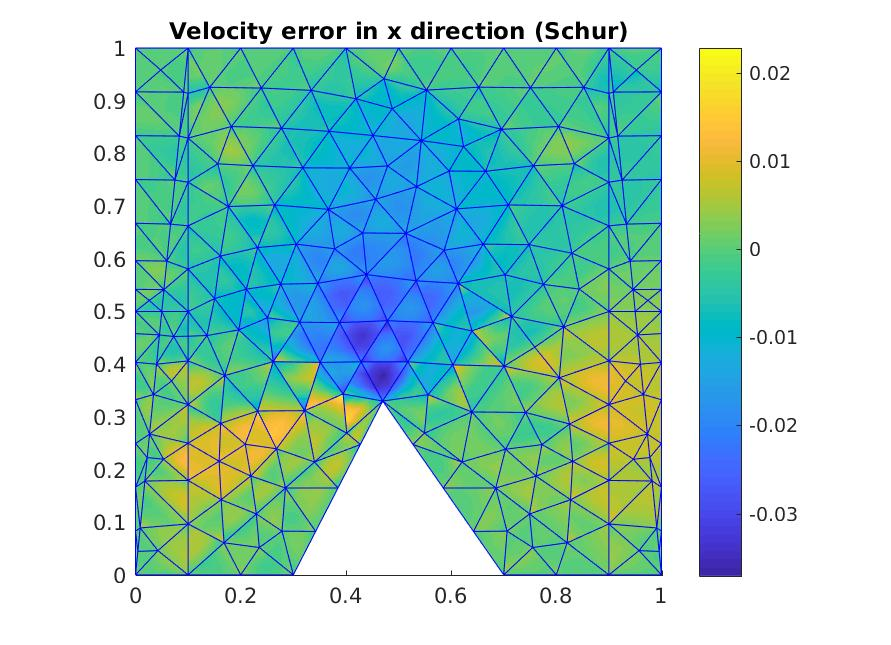
\includegraphics[width=\linewidth]{velocity_error_1_at_47_33.jpg}
\caption{$x-$component of Velocity absolute error $\overrightarrow{u}-\overrightarrow{u}_N$} \label{error_x_vel}
\end{subfigure}

\begin{subfigure}{0.31\textwidth}
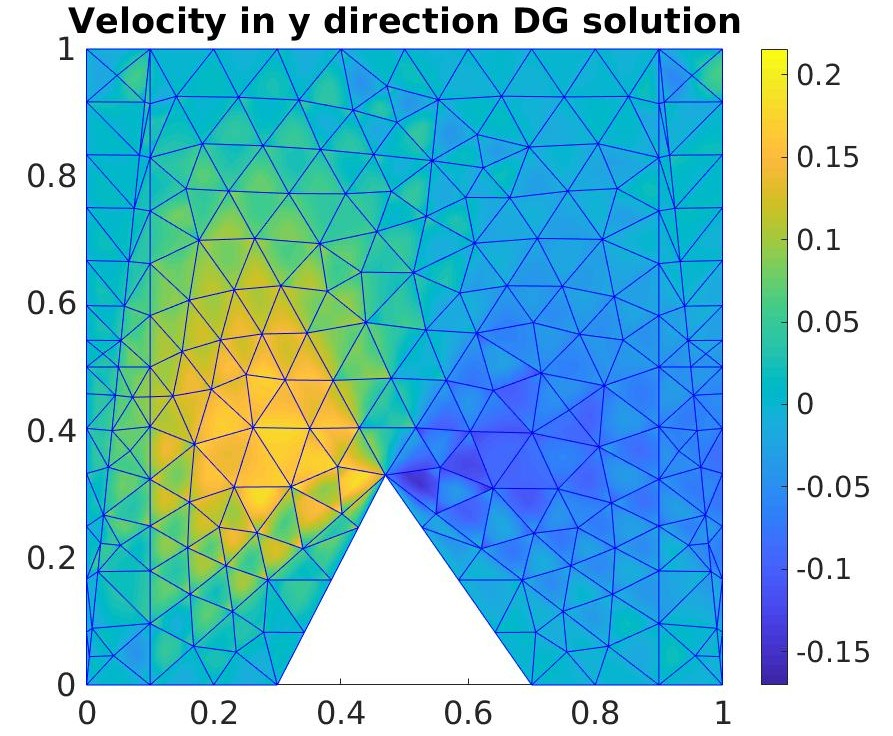
\includegraphics[width=\linewidth]{offline_velocity_2_at_47_33.jpg}
\caption{Velocity $y-$direction DG solution} \label{vel_y_dg}
\end{subfigure}\hspace*{\fill}
\begin{subfigure}{0.31\textwidth}
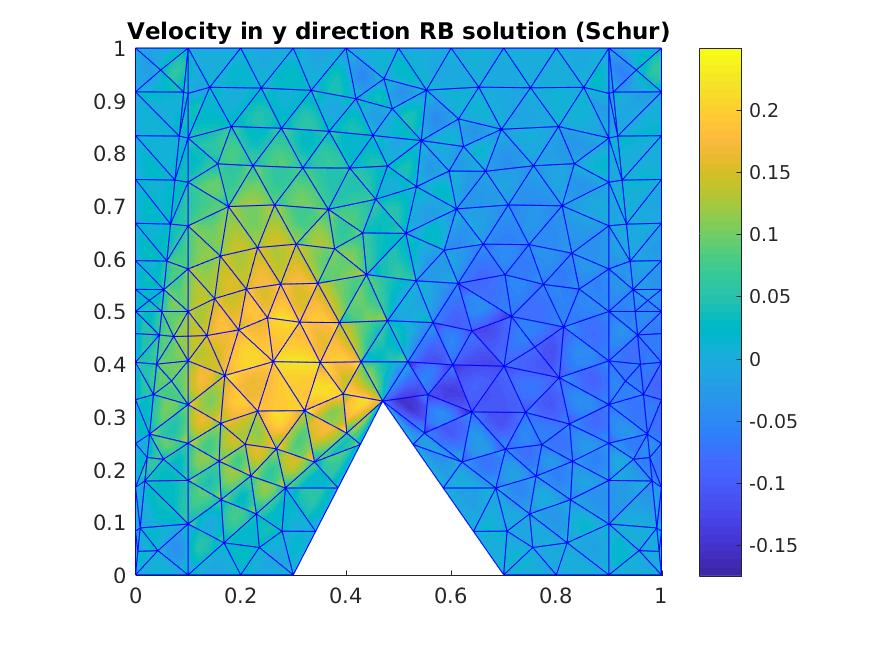
\includegraphics[width=\linewidth]{online_velocity_2_at_47_33.jpg}
\caption{Velocity $y-$direction RB solution} \label{vel_y_rb}
\end{subfigure}
\begin{subfigure}{0.31\textwidth}
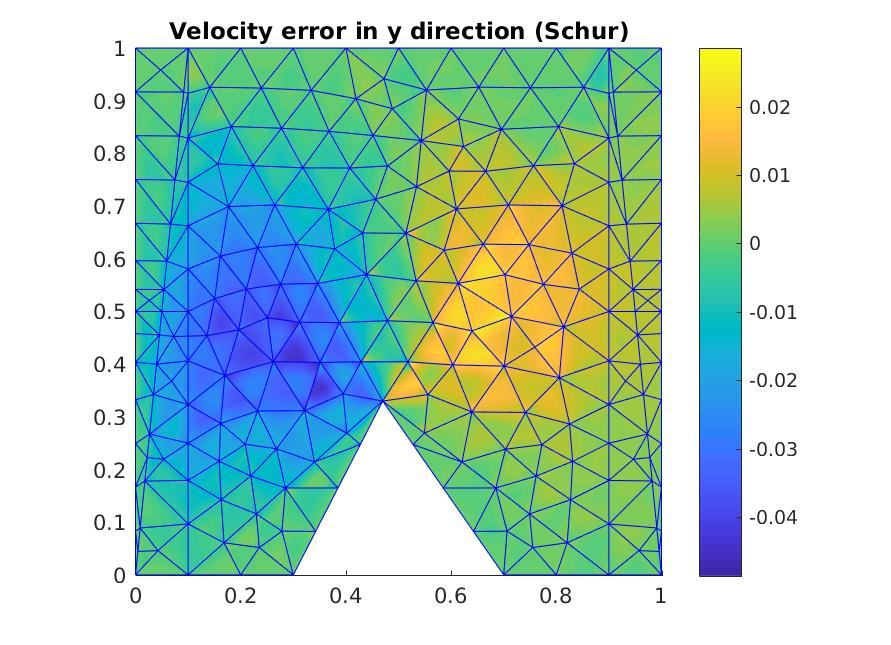
\includegraphics[width=\linewidth]{velocity_error_2_at_47_33.jpg}
\caption{$y-$component of Velocity absolute error $\overrightarrow{u}-\overrightarrow{u}_N$} \label{error_y_vel}
\end{subfigure}

\begin{subfigure}{0.31\textwidth}
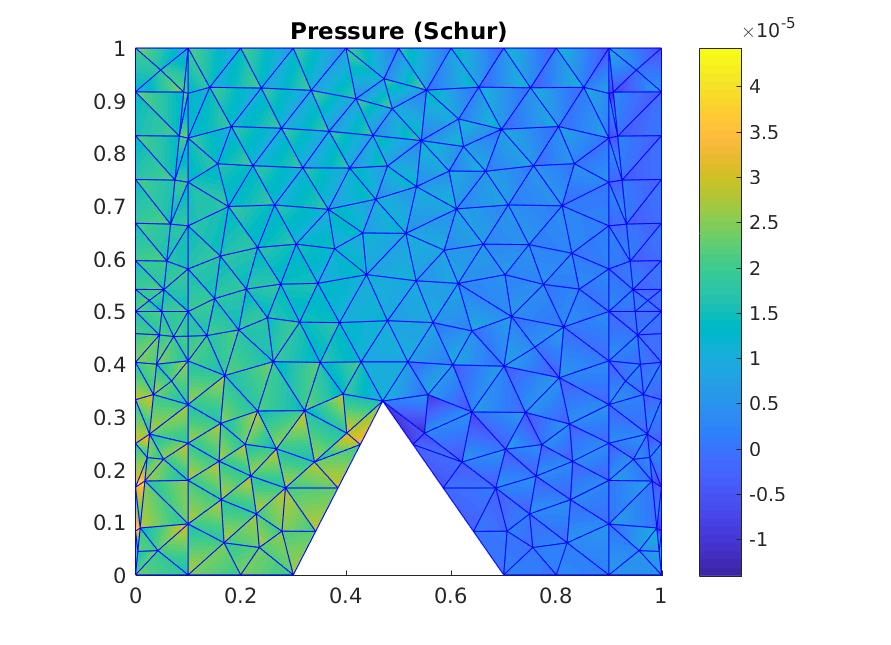
\includegraphics[width=\linewidth]{offline_pressure_at_47_33.jpg}
\caption{Pressure DG solution} \label{pre_dg}
\end{subfigure}\hspace*{\fill}
\begin{subfigure}{0.31\textwidth}
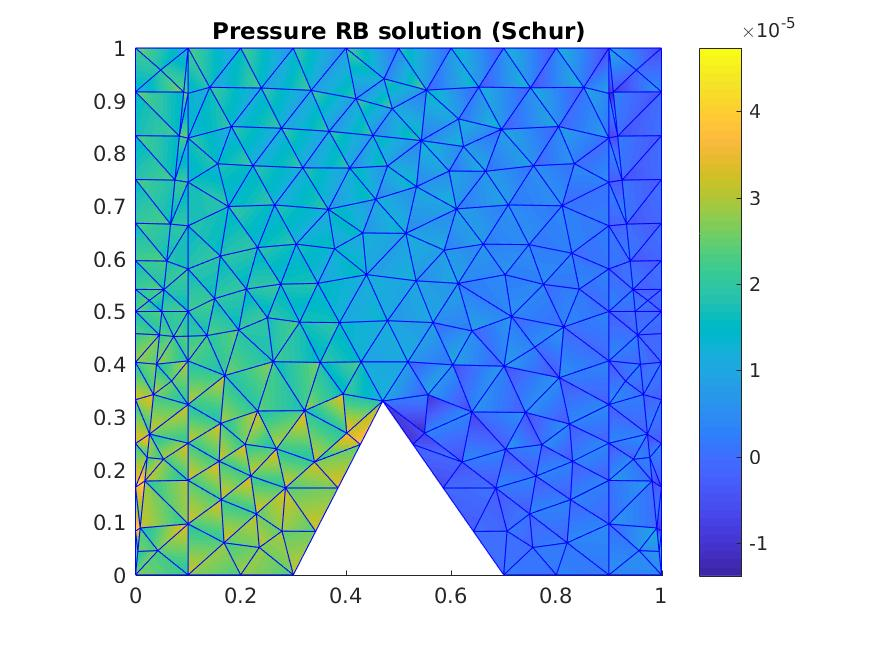
\includegraphics[width=\linewidth]{online_pressure_at_47_33.jpg}
\caption{Pressure RB solution} \label{pre_rb}
\end{subfigure}
\begin{subfigure}{0.31\textwidth}
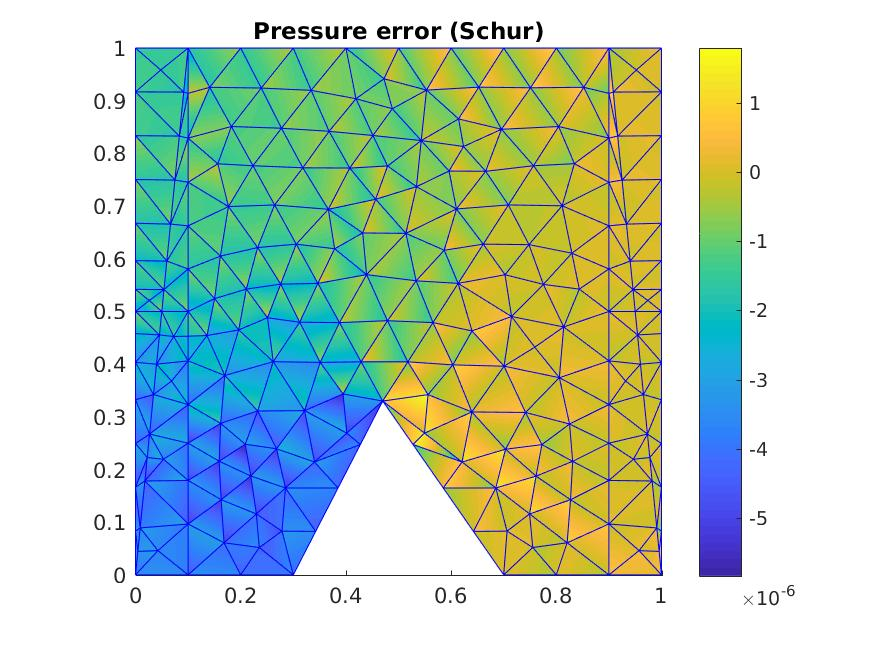
\includegraphics[width=\linewidth]{pressure_error_at_47_33.jpg}
\caption{Pressure absolute error $p-p_N$} \label{pre_error}
\end{subfigure}
\caption{DG and RB solution $[\mu_x \ \mu_y] = [0.47 \ 0.33]$} 
\label{dg_rb_solution_47_33}
\end{figure}

\begin{figure}
\begin{subfigure}{0.48\textwidth}
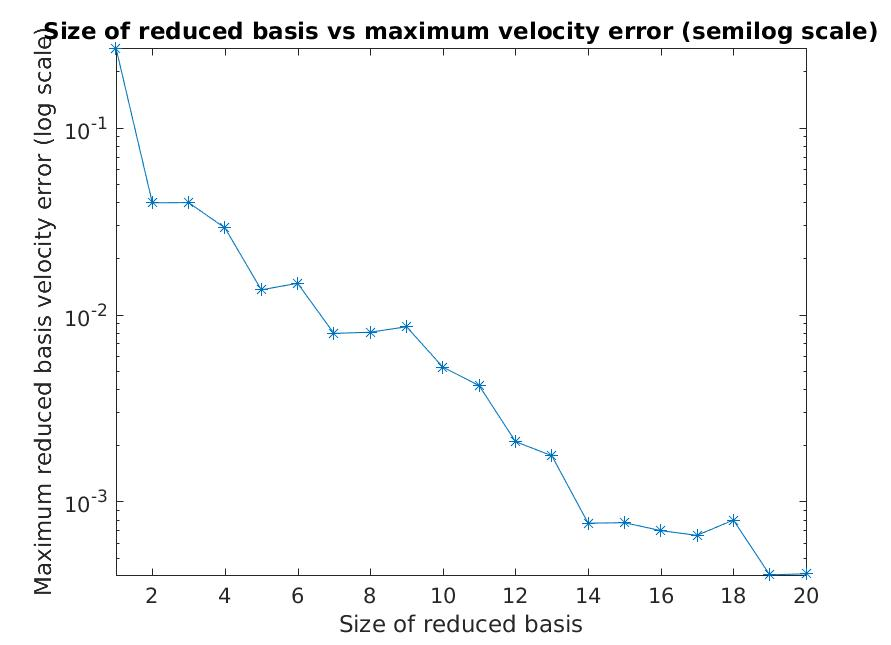
\includegraphics[width=\linewidth]{size_vs_maximum_reduced_basis_velocity_error_semilog.jpg}
\caption{Size of reduced basis space vs. Maximum relative error in velocity with inner product induced by $\bm{M}_v$} \label{error_vs_basis_velocity}
\end{subfigure}\hspace*{\fill}
\begin{subfigure}{0.48\textwidth}
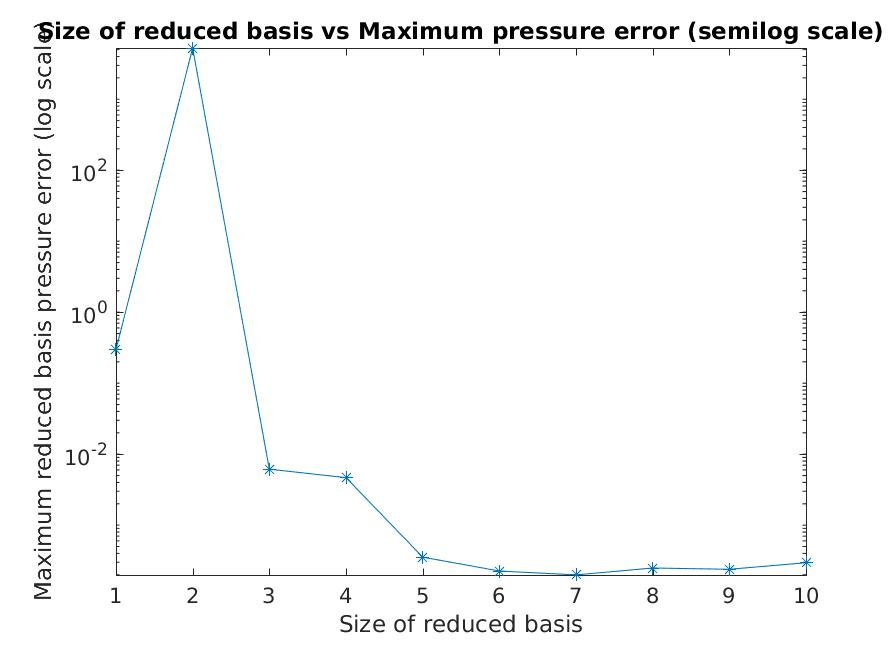
\includegraphics[width=\linewidth]{size_vs_maximum_reduced_basis_pressure_error_semilog.jpg}
\caption{Size of reduced basis space vs. Maximum relative error in pressure with inner product induced by $\bm{M}_p$} \label{error_vs_basis_pressure}
\end{subfigure}
  \caption{Size of reduced basis vs Maximum relative error} 
\label{error_vs_basis}
\end{figure}

\begin{figure}
\begin{subfigure}{0.48\textwidth}
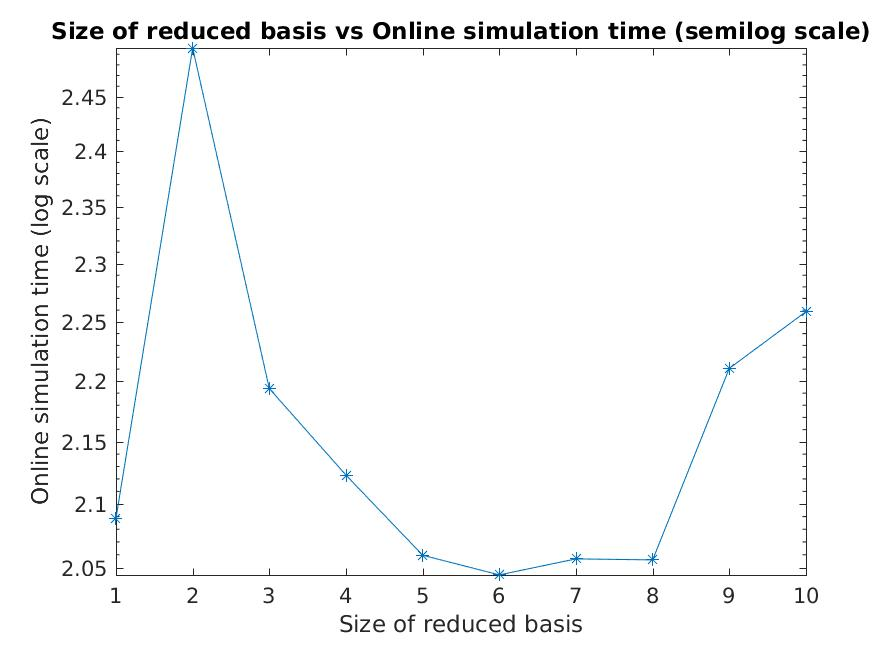
\includegraphics[width=\linewidth]{size_vs_online_simulation_time_semilog.jpg}
\caption{Size of reduced basis vs Online simulation time (semilog scale)} \label{online_simulation_time_vs_basis}
\end{subfigure}\hspace*{\fill}
\begin{subfigure}{0.48\textwidth}
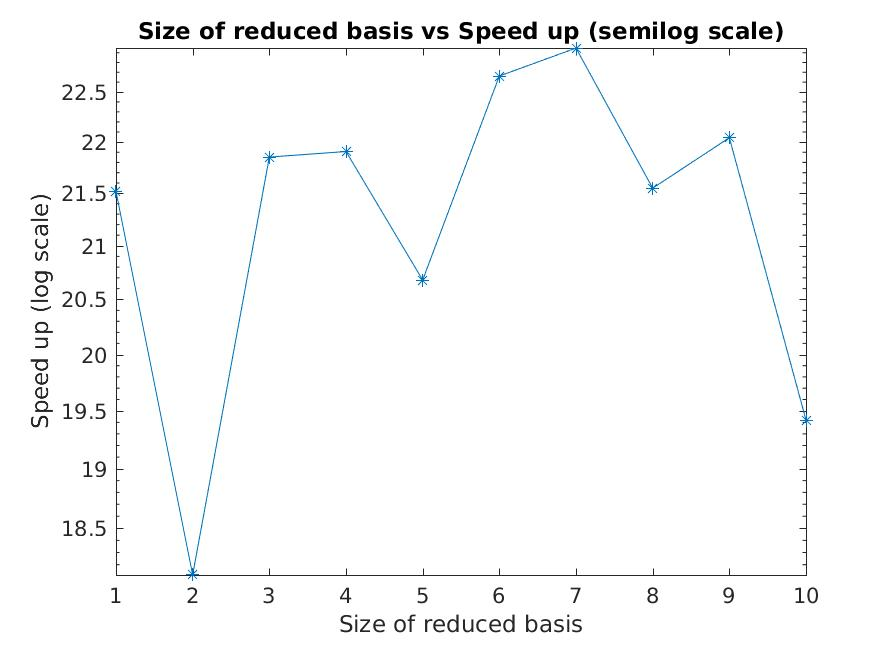
\includegraphics[width=\linewidth]{size_vs_reduced_basis_semilog.jpg}
\caption{Size of reduced basis vs Speed up (semilog scale)} \label{time_vs_speedup}
\end{subfigure}
\caption{Size of reduced basis for velocity vs Online computational time} 
\label{basis_vs_time}
\end{figure}

\bibliographystyle{spbasic.bst}
\bibliography{references.tex}
%%%%%%%%%%%%%%%%%%%% author.tex %%%%%%%%%%%%%%%%%%%%%%%%%%%%%%%%%%%
%
% sample root file for your "contribution" to a contributed volume
%
% Use this file as a template for your own input.
%
%%%%%%%%%%%%%%%% Springer %%%%%%%%%%%%%%%%%%%%%%%%%%%%%%%%%%


% RECOMMENDED %%%%%%%%%%%%%%%%%%%%%%%%%%%%%%%%%%%%%%%%%%%%%%%%%%%
\documentclass[graybox]{svmult}

% choose options for [] as required from the list
% in the Reference Guide

\usepackage{type1cm}        % activate if the above 3 fonts are
                            % not available on your system
%
\usepackage{makeidx}         % allows index generation
\usepackage{graphicx}        % standard LaTeX graphics tool
                             % when including figure files
\usepackage{multicol}        % used for the two-column index
\usepackage[bottom]{footmisc}% places footnotes at page bottom


\usepackage{newtxtext}       % 
\usepackage{newtxmath}       % selects Times Roman as basic font

\usepackage{url}

%%Nirav added
\newenvironment{spmatrix}[1]
 {\def\mysubscript{#1}\mathop\bgroup\begin{pmatrix}}
 {\end{pmatrix}\egroup_{\textstyle\mathstrut\mysubscript}}
\DeclareMathOperator{\Tr}{Tr}
\DeclareMathOperator{\spn}{span}
\usepackage{bm}
\usepackage{tikz}
\usepackage{wrapfig}
\usepackage[export]{adjustbox}
\usepackage{subcaption}
\usepackage{natbib}
\captionsetup{compatibility=false}
%%Nirav added over

% see the list of further useful packages
% in the Reference Guide

\makeindex             % used for the subject index
                       % please use the style svind.ist with
                       % your makeindex program

%%%%%%%%%%%%%%%%%%%%%%%%%%%%%%%%%%%%%%%%%%%%%%%%%%%%%%%%%%%%%%%%%%%%%%%%%%%%%%%%%%%%%%%%%

\begin{document}

\title{Discontinuous Galerkin model order reduction of geometrically parametrized Stokes flow}
% Use \titlerunning{Short Title} for an abbreviated version of
% your contribution title if the original one is too long
\author{Nirav Vasant Shah, Martin Hess and Gianluigi Rozza}
% Use \authorrunning{Short Title} for an abbreviated version of
% your contribution title if the original one is too long
\institute{Nirav Vasant Shah \at Scuola Internazionale Superiore di Studi Avanzati - via Bonomea, 265 - 34136 Trieste ITALY, \email{snirav@sissa.it}
\and Martin Hess \at Scuola Internazionale Superiore di Studi Avanzati - via Bonomea, 265 - 34136 Trieste ITALY \email{martin.hess@sissa.it}}
%
% Use the package "url.sty" to avoid
% problems with special characters
% used in your e-mail or web address
%
\maketitle

\abstract*{Each chapter should be preceded by an abstract (no more than 200 words) that summarizes the content. The abstract will appear \textit{online} at \url{www.SpringerLink.com} and be available with unrestricted access. This allows unregistered users to read the abstract as a teaser for the complete chapter.
Please use the 'starred' version of the \texttt{abstract} command for typesetting the text of the online abstracts (cf. source file of this chapter template \texttt{abstract}) and include them with the source files of your manuscript. Use the plain \texttt{abstract} command if the abstract is also to appear in the printed version of the book.}

\abstract{The present work focuses on geometrical parametrization and reduced order modeling of Stokes flow. We discuss the concept of geometric parametrization and its application along with importance of reduced order model technique.  The full order model is based on discontinuous Galerkin method interior penalty formulation. We introduce broken Sobolev spaces, relevant norms, jump and mean operator, weak formulation. The operators are transformed from fixed domain to parameter dependent domain by exploring affine parameter dependence. Proper orthogonal decomposition is applied to geometrically parametrized Stokes flow to obtain basis of function space for reduced order model. By using Galerkin projection the linear system is projected onto reduced space. During the process, offline-online decomposition is used to separate parameter independent and parameter independent operations. Finally the technique is applied to a test problem. The numerical outcomes presented include the experimental error analysis and measurement of online simulation time. \cite{psysoc-journal}\\
\textbf{Keywords:} Discontinuous Galerkin method, Stokes flow, Geometric parametrization, Proper orthogonal decomposition }

\section{Introduction}
\label{introduction}

The subject of mathematical applications in fluid mechanics starts with one of the variants of the Navier-Stokes equations, such as the Stokes equation. Almost all processes of fluid mechanics require considerations related to the Navier-Stokes equations. Navier-Stokes equation is non-linear, characterizing flow fluctuations. However, in case of laminar flow, i.e. when fluctuations are negligible, this linearized form of the Navier-Stokes equation is the Stokes equation.

Discontinuous Galerkin method (DGM) has found traction as numerical method for elliptic problems \textbf{pereire reference} as well as hyperbolic problems \textbf{Book on compressible flow reference}. This is due to its several advantages over Finite Element Method (FEM) and Finite Volume Method (FVM). In fact, DGM is considered as combination of FEM and FVM. DGM uses polynomial approximation of suitable degree providing higher accuracy as well as allows discontinuity at the interface, by the concept of numerical flux, allowing greater flexibility. This fact makes DGM naturally attractive to problems, such as shock capturing, due to presence of steep gradients or discontinuities. Additionally, since the Dirichlet conditions are applied as boundary penalty, it avoids necessity to work with subspace of Sobolev space such as in case of FEM. Several variants of DGM exist based on computational advantages such as sparsity pattern or extension of computational stencil, complexity of numerical implementation etc.

Geometric parametrization has emerged as important application of Parametric Partial Differential Equations (PPDEs) and as alternative to shape optimization. The concept of geometric parametrization allows to transfer operator evaluated on one geometric domain to another geometric domain efficiently. For linear equations, this means exploiting affine parameter dependence as will be shown in later section. Model Order Reduction (MOR) on the other hand allows reducing the size of the system to be solved and working with the smaller system containing only dominant components and discarding the non-dominant components. It is pertinent to mention that identifying "dominant" components is critical to the success of model order reduction strategy. Optimization of engineering components using geometric parametrization combined with MOR for PPDEs has given quite useful results in the fields such as mechanical, naval and aeronautic designs. Also, the  faster computations obtained by MOR has helped in many query context, real time computation and quick transfer of computational results to industrial problems.

In the present work, we first introduce notion of parametrization characterizing geometry of the domain under consideration. We subsequently introduce Discontinuous Galerkin Interior Penalty Method (DG-IPM) for stokes flow. We then explain exploiting affine parameter dependence and its application in the context of offline-online decomposition. We then apply Proper Orthogonal Decomposition (POD) for constructing reduced basis space and apply Galerkin projection to project the system of equations on the space constructed by POD. Finally we present a test problem to demonstrate the introduced method and numerical result.

\section{Geometric parametrization}\label{geometric_parametrization_section}

Consider domain $\Omega = \Omega(\mu) \in \mathbb{R}^d$ as open bounded domain. The parameter set $\mu \in \mathbb{P}$, where $\mathbb{P}$ is parameter space, completely characterizes the domain. Also, consider a parameter set $\bar{\mu} \in \mathbb{P}$, as the known parameter set and $\Omega(\bar{\mu})$ as the reference domain, whose configuration is completely known. The mapping $\bm{F}(\cdot,\mu) : \Omega(\bar{\mu}) \rightarrow \Omega(\mu)$ links reference domain and parametrized domain. Divide the domain $\Omega(\mu)$ into $n_{su}$ subdomains such that $\Omega(\mu) = \bigcup\limits_{i=1}^{n_{su}} \Omega_i(\mu) \ , \ \Omega_i(\mu) \bigcap \Omega_j(\mu) = \emptyset \ , \ \text{for} \ i \neq j$. The boundary of $\Omega(\mu)$, that is $\partial \Omega(\mu)$ is divided into Neumann boundary $\Gamma_N(\mu)$ and Dirichlet boundary $\Gamma_D(\mu)$ i.e. $\partial \Omega(\mu) = \Gamma_N(\mu) \cup \Gamma_D(\mu)$.

In the case of affine transformation, $\bm{F}$ is of the form,
\begin{gather}\label{affine_F}
x = \bm{F}(\hat{x},\mu) = \bm{G}_F(\mu)\hat{x} + c_F(\mu) \ ; \forall x \in \Omega \ , \ \hat{x} \in \Omega(\bar{\mu}) \ .
\end{gather}

The inverse map $\bm{T}$ is expressed in the form,
\begin{gather}\label{affine_T}
\hat{x} = \bm{T}(x,\mu) = \bm{G}_T(\mu)x + c_T(\mu) \ ; \forall x \in \Omega \ , \ \hat{x} \in \Omega(\bar{\mu}) \ .
\end{gather}

\section{Discontinuous Galerkin formulation}
\label{DG_formulation}

Each subdomain is divided into $N_{el}$ number of triangular elements $\tau_k$ such that $\Omega = \bigcup\limits_{k=1}^{N_{el}} \tau_k$. The triangulation $\mathcal{T}$ is the set of all triangular elements i.e. $\mathcal{T} = \lbrace \tau_k \rbrace_{k=1}^{N_{el}}$. The internal boundary $\Gamma = \lbrace \bigcup\limits_{k=1}^{N_{el} \partial \tau_k \rbrace} \backslash \partial \Omega$. The vertices of triangle ${\tau_k}_{k=1}^{N_{el}}$ are called nodes. $\overrightarrow{n}$ is the outward pointing normal to an edge of element.

The Stokes's equation in strong form can be stated as,
\begin{gather}\label{stokes_strong_form}
-\nu \Delta \overrightarrow{u} + \nabla p = \overrightarrow{f} \ , \ \text{in } \Omega \ , \\
\nabla \cdot \overrightarrow{u} = 0 \ , \ \text{in} \ \Omega \ , \\
\overrightarrow{u} = \overrightarrow{u}_D \ , \ \text{on } \Gamma_D \ , \\
-p \overrightarrow{n} + \nu \overrightarrow{n} \cdot \nabla \overrightarrow{u} = \overrightarrow{t} \ , \ \text{on} \ \Gamma_N \ .
\end{gather}

The velocity vector field $\overrightarrow{u}$ and pressure scalar field $p$ are the unknowns. $\nu$ is the material property known as kinematic viscosity. Vector $\overrightarrow{f}$ is external force term or source term. $\overrightarrow{u}_D$ is the Dirichlet velocity and $\overrightarrow{t}$ is the Neumann value.

Before introducing weak form let us introduce broken Sobolev spaces for variables.

The space for velocity is 
\begin{equation} \label{velocity_test}
\mathbb{V} = \lbrace \overrightarrow{\phi} \in (L^2(\Omega))^d | \ \overrightarrow{\phi} \in (P^D(\tau_k))^d \ , \ \tau_k \in \mathcal{T} \rbrace \ .
\end{equation}
The space for pressure is 
\begin{equation} \label{pressure_test}
\mathbb{Q} = \lbrace \psi \in (L^2(\Omega)) | \ \psi \in (P^{D-1}(\tau_k)) \ , \ \tau_k \in \mathcal{T} \rbrace \ .
\end{equation}
Here, $P^D(\tau_k)$ denotes space of polynomials of degree at most $D \geq 2$ over $\tau_k$.

The velocity $\overrightarrow{u}(x)$ and pressure $p(x)$ at any point $x \in \Omega$ is given by,
\begin{equation}\label{velocity_pressure_coefficients}
\overrightarrow{u}(x) = \sum\limits_{i=1}^{\overrightarrow{u}_{ndofs}} \overrightarrow{\phi}_i \hat{u}_i \ , \
p(x) = \sum\limits_{i=1}^{p_{ndofs}} \psi_i \hat{p}_i \ ,
\end{equation}
where $\hat{u}_i$'s and $\hat{p}_i$'s are coefficients of velocity basis functions and pressure basis functions respectively. 

\begin{figure}
\centering
\sidecaption[t]
\begin{tikzpicture}
\draw (0,0) node[anchor=north]{${}$}
  -- (4,0) node[anchor=north]{${}$}
  -- (0,4) node[anchor=south]{${}$}
  -- cycle;
\draw (4,4) node[anchor=north]{${}$}
  -- (4,0) node[anchor=north]{${}$}
  -- (0,4) node[anchor=south]{${}$}
  -- cycle;
\draw[->] (2,2)--(2.5,2.5)node[label={[xshift=0.4cm, yshift=-0.7cm]${\overrightarrow{n}^-}$}]{};
\draw[->] (2,2)--(1.5,1.5)node[label={[xshift=0cm, yshift=0cm]${\overrightarrow{n}^+}$}]{};
\node at (1,1){$\tau_{k}^-$};
\node at (3,3){$\tau_{k}^+$};
\node at (1.7,3){$\overrightarrow{\phi}^+,\psi^+$};
\node at (2.3,1){$\overrightarrow{\phi}^-,\psi^-$};
\end{tikzpicture}
\caption{Definition of jump and mean operator. \newline The superscript $+$ refers to quantity in the element itself and the superscript $-$ refers to quantity in the neighboring element}
\label{fig:Self_neighbour}
\end{figure}

In the subsequent sections $\left( \cdot \right),\left( \cdot \right)_{\Gamma_D},\left( \cdot \right)_{\Gamma_N},\left( \cdot \right)_{\Gamma}$ represent the $L^2$ scalar product over $\Omega,\Gamma_D,\Gamma_N,\Gamma$ respectively. The jump operator $\left[ \cdot \right]$ and the average operator $\lbrace \cdot \rbrace$ are are important concepts in DGM formulation and are required to approximate the numerical flux (Figure \ref{fig:Self_neighbour}).

The presence of normal vector $\overrightarrow{n}$ in jump and average operator introduced below allows symmetric formulation and also ensures that jump of a vector is vector and jump of a scalar is scalar.

\begin{itemize}
\item For vector quantity $\overrightarrow{\phi}$:
\begin{itemize}
\item Jump operator: 
$\left[\overrightarrow{\phi} \cdot \overrightarrow{n}\right] = \overrightarrow{\phi}^+ \cdot \overrightarrow{n}^+ + \overrightarrow{\phi}^- \cdot \overrightarrow{n}^-$ on $\Gamma$, $\left[\overrightarrow{\phi} \cdot \overrightarrow{n}\right] = \overrightarrow{\phi} \cdot \overrightarrow{n}$ on $\partial \Omega$.
\item Average operator:
$\lbrace \overrightarrow{\phi} \rbrace = \frac{\overrightarrow{\phi}^+ + \overrightarrow{\phi}^-}{2}$ on $\Gamma$, $\lbrace \overrightarrow{\phi} \rbrace = \overrightarrow{\phi}$ on $\partial \Omega$.
\end{itemize}
\item For scalar quantity $\psi$:
\begin{itemize}
\item Jump operator:
$\left[\psi \overrightarrow{n} \right] = \psi^+ \overrightarrow{n}^+ + \psi^- \overrightarrow{n}^-$ on $\Gamma$, $\left[\psi \overrightarrow{n} \right] = \psi \overrightarrow{n}$ on $\partial \Omega$.
\item Average operator:
$\lbrace \psi \rbrace = \frac{\psi^+ + \psi^-}{2}$ on $\Gamma$, $\lbrace \psi \rbrace = \psi$ on $\partial \Omega$. 
\end{itemize}
\end{itemize}

The weak form of Stokes equation is as follow,
\begin{gather}\label{stokes_weak_ch3}
a_{IP}(\overrightarrow{u},\overrightarrow{\phi}) + b(\overrightarrow{\phi},p) + \left( \lbrace p \rbrace,[\overrightarrow{n} \cdot \overrightarrow{\phi}] \right)_{\Gamma \cup \Gamma_D} = l_{IP}(\overrightarrow{\phi}) \ , \\
a_{IP}(\overrightarrow{u},\overrightarrow{\phi}) = \left( \nabla \overrightarrow{u}, \nabla \overrightarrow{\phi} \right) + C_{11} \left( [\overrightarrow{u}],[\overrightarrow{\phi}] \right)_{\Gamma \cup \Gamma_D} - \nu \left( \lbrace \nabla \overrightarrow{u}\rbrace ,[\overrightarrow{n} \otimes \overrightarrow{\phi}] \right)_{\Gamma \cup \Gamma_D} - \nu \left( [\overrightarrow{n} \otimes \overrightarrow{u}], \lbrace \nabla \overrightarrow{\phi} \rbrace \right)_{\Gamma \cup \Gamma_D} \ , \\
b(\phi,\psi) = -\int_{\mathcal{T}} \psi \nabla \cdot \overrightarrow{\phi} \ , \\
l_{IP}(\overrightarrow{\phi}) = \left( \overrightarrow{f},\overrightarrow{\phi} \right) + \left( \overrightarrow{t},\overrightarrow{\phi} \right)_{\Gamma_N} + C_{11} \left(\overrightarrow{u}_D,\overrightarrow{\phi}\right)_{\Gamma_D} - \left( \overrightarrow{n} \otimes \overrightarrow{u}_D, \nu \nabla \overrightarrow{\phi} \right)_{\Gamma_D} \ .
\end{gather}

The penalty parameter $C_{11}>0$ in $a_{IP}(\overrightarrow{u},\overrightarrow{\phi})$ is an empirical constant to be kept large enough to maintain coercivity of bilinear form.

The weak for of continuity equation is as follow,
\begin{equation}\label{contiuity_weak_ch3}
\begin{split}
b(\overrightarrow{u},\psi) + ({\psi},[\overrightarrow{n} \cdot \overrightarrow{u}])_{\Gamma \cup \Gamma_D} = (\psi,\overrightarrow{n} \cdot \overrightarrow{u}_D)_{\Gamma_D} \ .
\end{split}
\end{equation}

In discrete form system of equations can be written as, 
\begin{equation} \label{Stokes_matrix_ch3}
\begin{spmatrix}{\textrm{Stiffness matrix}}
    \bm{A} & \bm{B} \\
    \bm{B}^T & 0
\end{spmatrix}
\begin{spmatrix}{\textrm{Solution vector}}
    U \\
    P
\end{spmatrix}
=
\begin{spmatrix}{\textrm{Right hand side (Known)}}
    F_1  \\
    F_2
\end{spmatrix}
\textrm{.}
\end{equation}

Here, $\bm{A}_{ij} = a_{IP} (\overrightarrow{\phi}_i,\overrightarrow{\phi}_j)$, $\bm{B}_{ij} = b(\overrightarrow{\phi}_i,\psi_j) + \left( \lbrace \psi_j \rbrace , [n \cdot \phi_i]\right)_{\Gamma \cup \Gamma_D}$, $F_1 = l_{IP}(\overrightarrow{\phi}_i)$ and $F_2 = \left( \psi_j,\overrightarrow{n} \cdot \overrightarrow{u}_D \right)_{\Gamma_D}$. The column vectors $U$ and $P$ are coefficients $\hat{u}$'s and $\hat{p}$'s from equation \eqref{velocity_pressure_coefficients}.

\section{Affine expansion}

We evaluate and solve the Stokes equation weak formulation on reference domain $\Omega{\bar{\mu}}$. Given a parameter set $\mu \neq \bar{\mu}$ we need to evaluate the linear systems of equation \eqref{Stokes_matrix_ch3} on new domain $\Omega(\mu)$. To accomplish this we use affine expansion using linear nature of equation and diving $\Omega(\bar{\mu})$ into triangular subdomains $\Omega_i(\bar{\mu}) \ , \ i = \lbrace 1,2,\ldots,n_{su} \rbrace$ as explained earlier in the section geometric parametrization [Section \ref{geometric_parametrization_section}]. The affine expansion of operators is essentially change of variable and has been explained in literatures such as \textbf{ADD affine expansion literature}. However it is pertinent to mention two expansions as specific to DGM formulation will be mentioned here as below.

\begin{itemize}
\item In order to transfer the terms containing jump and average operator following approach is used in present analysis.
\begin{equation*}\label{jump_average_term_split}
\begin{split}
\left(\lbrace \nabla \overrightarrow{\phi} \rbrace , \left[ \overrightarrow{n} \otimes \overrightarrow{\phi}  \right]  \right) = \left( \nabla \overrightarrow{\phi}^+ , \overrightarrow{n}^+ \otimes \overrightarrow{\phi}^+ \right) + \left( \nabla \overrightarrow{\phi}^+ , \overrightarrow{n}^- \otimes \overrightarrow{\phi}^- \right) + \\ 
\left( \nabla \overrightarrow{\phi}^- , \overrightarrow{n}^+ \otimes \overrightarrow{\phi}^+ \right) + \left( \nabla \overrightarrow{\phi}^- , \overrightarrow{n}^- \otimes \overrightarrow{\phi}^- \right) \ .
\end{split}
\end{equation*}
Each term on right hand side of equation \eqref{jump_average_term_split} can now be transformed using affine map.

\item The coercivity term $C_{11}\left( [\overrightarrow{\phi}],[\overrightarrow{u}] \right)_{\Gamma \cup \Gamma_D}$ is not transformed but used as evaluated on reference domain $\Omega(\bar{\mu})$. The affine transformation is given by,
\begin{equation*}
\begin{split}
C_{11}\left( [\overrightarrow{\phi}(\hat{x}),\overrightarrow{u}(\hat{x})] \right)_{\Gamma(\mu) \cup \Gamma_D(\mu)} = C_{11} \alpha \left( [\overrightarrow{\phi}(\bm{F}(\hat{x})),\overrightarrow{u}(\bm{F}(\hat{x}))] \right)_{\Gamma(\bar{\mu}) \cup \Gamma_D(\bar{\mu})} \ , \\
\alpha = \frac{meas\left( \Gamma(\mu) \cup \Gamma_D(\mu)\right)}{meas\left( \Gamma(\bar{\mu}) \cup \Gamma_D(\bar{\mu})\right)} \ , \ \hat{x} \in \Omega(\bar{\mu}) \ , \ x \in \Omega(\mu) \ .
\end{split}
\end{equation*}

Since, $C_{11}$ is empirical coefficient replacing $C_{11} \alpha$ with $C_{11}$ will not change the formulation as long as coercivity of $a_{IP}$ over parameter space $\mathbb{P}$ is maintained. In the present analysis, $C_{11}$ is not calculated exactly but only order of magnitude required for $C_{11}$ is estimated and $C_{11}$ is kept one magnitude larger as safeguard against round-off errors. As long as the domain $\Omega(\mu)$ is not deformed much compared to its reference configuration $\Omega(\bar{\mu})$, $C_{11}$ and $C_{11}\alpha$ will have the same order of magnitude. However, regardless of this fact, large deformations are not favorable as it will lead to bad mesh quality and in turn, will lead to poor DGM-approximation.
\end{itemize}

\section{Reduced basis method}

\subsection{Snapshot proper orthogonal decomposition}\label{POD_section}

We present now snapshot proper orthogonal decomposition method. Here, ``snapshot" means solution calculated by discontinuous Galerkin method. We calculate solution based on $\mu_n, n \in \lbrace 1,....,n_s \rbrace$ i.e. $n_s$ snapshots are generated. We also introduce inner product matrices $\bm{M}_v \in \mathbb{R}^{\overrightarrow{u}_{ndofs} \times \overrightarrow{u}_{ndofs}}$ and $\bm{M}_p \in \mathbb{R}^{p_{ndofs} \times p_{ndofs}}$.

\begin{gather*}
\bm{M}_v = \int_{\Omega} \overrightarrow{\phi}_i \cdot \overrightarrow{\phi}_j + \sum_{k=1}^{N_{el}} \int_{\tau_k} \nabla \overrightarrow{\phi}_i : \nabla \overrightarrow{\phi}_j \ , \ i,j = 1, \ldots, \overrightarrow{u}_{ndofs} \ , \\
\bm{M}_p = \int_{\Omega} \psi_i \psi_j \ , \ i,j = 1, \ldots, p_{ndofs} \ .
\end{gather*}

We also introduce matrices storing velocity snapshots $\bm{S}_v$ and storing pressure snapshots $\bm{S}_p$. We discuss the method only for velocity snapshots. The method is similar for pressure snapshots. We note the size of matrices, useful for matrix operations presented hereafter.

\begin{gather*}
\bm{S}_v \in \mathbb{R}^{\overrightarrow{u}_{ndofs} \times n_s} \ , \ \bm{S}_p \in \mathbb{R}^{p_{ndofs} \times n_s} \ , \\
\bm{M}_v \in \mathbb{R}^{\overrightarrow{u}_{ndofs} \times \overrightarrow{u}_{ndofs}} \ ,\ \bm{M}_p \in \mathbb{R}^{p_{ndofs} \times p_{ndofs}} \ .
\end{gather*}

\subsection{Spectral decomposition of snapshots}\label{spectral_decomposition_section}

We denote the dimension of reduced basis as $N$ and assert that $N << n_s$. We now perform the spectral decomposition of $\bm{S}_v^T \bm{M}_v \bm{S}_v$,

\begin{equation}\label{snapshot_eigen_value}
\bm{S}_v^T \bm{M}_v \bm{S}_v = \bm{V} \bm{\Theta} \bm{V}^T \ .
\end{equation}

The columns of $V$ are eigenvectors and $\Theta$ has eigenvalues $\theta_i \ , \ 1 \leq i \leq n_s$ such that,
\begin{equation}
\Theta_{ij} = \theta_i \delta_{ij} \ .
\end{equation}

We also note that $\theta_i > 0$ and $\theta_1 \geq \theta_2 \geq ... \geq \theta_{n_s}$ i.e. the eigenvalues are in sorted order. We form the reduced basis by linear combination of the snapshot vector,
\begin{equation}\label{linear_combination_snapshots}
\bm{B}_v = \bm{S}_v \bm{A} \ , \ \bm{A} \in \mathbb{R}^{n_s \times N} \ .
\end{equation}
the reduced basis for velocity basis function $\overrightarrow{\phi}_N$ is formed by,
\begin{equation}
\overrightarrow{\phi}_N = \overrightarrow{\phi}^T \bm{B}_v \ .
\end{equation}

Considering orthonormality of reduced basis $\overrightarrow{\phi}_N$ with respect to inner product induced by $\bm{M}_v$, from equation \eqref{snapshot_eigen_value},
\begin{equation}
<\overrightarrow{\phi}_N,\overrightarrow{\phi}_N>_{\bm{M}_v} = \bm{B}_v^T \bm{M}_v \bm{B}_v = I \ .
\end{equation}
From equation \eqref{linear_combination_snapshots}, we express matrix $\bm{A}$ as,
\begin{equation}
\bm{A} = \bm{V} \bm{\Theta}^{-\frac{1}{2}} \bm{R} \ , \ \bm{R} = [\bm{I}_{N \times N} ; \bm{0}_{(N-n_s \times N)}] \ \text{and accordingly} \ \bm{B}_v = \bm{S}_v \bm{V} \bm{\Theta}^{-\frac{1}{2}} \bm{R} \ .
\end{equation}
The columns of $\bm{B}_v$ now represent the basis functions for reduced space for velocity. Due to round-off errors, these basis functions may not be of unit magnitude and it is necessary to normalize the basis functions.

The reduced basis space $\bm{B}_p$ can be generated in similar manner using pressure snapshots $\bm{S}_p$ and inner product matrix $\bm{M}_p$.

\subsection{Galerkin reduced basis formulation}\label{Galerkin_section}

We now present the reduced bilinear form as,

\begin{equation} \label{stokes_equation_parameter}
a(u_N,\phi_N;\mu) + b(p_N,\phi_N;\mu) = f_1(\phi_N,\mu) \textrm{,}
\end{equation}

\begin{equation} \label{continuity_equation_parameter}
b(u_N,\psi_N;\mu) = f_2(\psi_N,\mu) \textrm{.}
\end{equation}

In discrete form, we form reduced equation as,

\begin{equation} \label{Stokes_matrix_reduced}
\begin{spmatrix}{\tilde{K}}
    \bm{B}_v^T \bm{A}(\mu) \bm{B}_v & \bm{B}_v^T \bm{B}(\mu) \bm{B}_v \\
    \bm{B}_p^T \bm{B}(\mu)^T \bm{B}_v & \bm{0}
\end{spmatrix}
\begin{spmatrix}{\zeta}
    U_N \\
    P_N
\end{spmatrix}
=
\begin{spmatrix}{\tilde{F}}
    \bm{B}_v^T F_1(\mu)  \\
    \bm{B}_p^T F_2(\mu)
\end{spmatrix} \ ,
\end{equation}
and accordingly we solve following variational form for reduced degrees of freedom $\zeta$,
\begin{equation}
\tilde{\bm{K}} \zeta = \tilde{F} \ ,
\end{equation}
and calculate reduced solutions $\overrightarrow{u}_N$ and $p_N$ as,
\begin{equation}
\overrightarrow{u}_N = \bm{B}_v U_N \ , \ p_N = \bm{B}_p P_N
\end{equation}

\section{Offline-online procedure}

The offline-online procedure is used to separate computationally intensive parameter independent offline procedure and faster parameter dependent online procedure \textbf{cite CRBM}. During the offline phase $n_s$ snapshots are computed and reduced basis spaces $\bm{B}_v$ and $\bm{B}_p$ are created. The offline procedure is outlined in section \ref{POD_section} and section \ref{spectral_decomposition_section}. During the online phase the systems of equations are projected on reduced space using Galerkin projection, the smaller systems of equation obtained by Galerkin projection is solved and the reduced basis solution is computed as outlined in section \ref{Galerkin_section}. The parameter dependent matrices in equation \eqref{Stokes_matrix_reduced} are evaluated by using affine decomposition.

\section{Numerical example}

We perform the POD-Galerkin method as mentioned in section \ref{POD_section} - section \ref{Galerkin_section}. The reference domain $\Omega{\bar{\mu}}$ is the unit square domain with triangle with vertices $(0.3,0),(0.5,0.3),(0.7,0)$ as obstacle. The geometric parameters are coordinates of tip of the obstacle i.e. $\bar{\mu} = (0.5,0.3)$. The boundary ${x=0}$ is Dirichlet boundary with inflow velocity at point $(0,y)$ as $u = (y(1-y), 0)$. The boundary ${x = 1}$ is a Neumann boundary with zero Neumann value i.e. $t = (0, 0)$. Other boundaries are Dirichlet boundary with no slip condition. The source term is $f = (0,0)$.

The training set was generated by random generation of $100$ parameters between the interval $[0.4,0.6] \times [0.4,0.6]$. The test set contained $10$ random parameters between the interval $[0.4,0.6] \times [0.4,0.6]$. For velocity basis function polynomial of degree $P^D = 2$ and for pressure basis function polynomial of degree $P^{D-1} = 1$ was used. The number of velocity degrees of freedom and pressure degrees of freedom were $\overrightarrow{u}_{ndofs} = 4704$ and $p_{ndofs} = 1176$ respectively.

Figure \ref{dg_rb_solution_47_33} shows solution computed by DGM and POD at parameter value $(0.47,33)$. Figure \ref{error_vs_basis} shows error vs size of reduced basis space. As can be seen the error drops with increasing size of basis function, however, this has to be at affordable cost of increased online simulation time (Figure \ref{basis_vs_time}).

\begin{figure}%[t!] % "[t!]" placement specifier just for this example
\begin{subfigure}{0.31\textwidth}
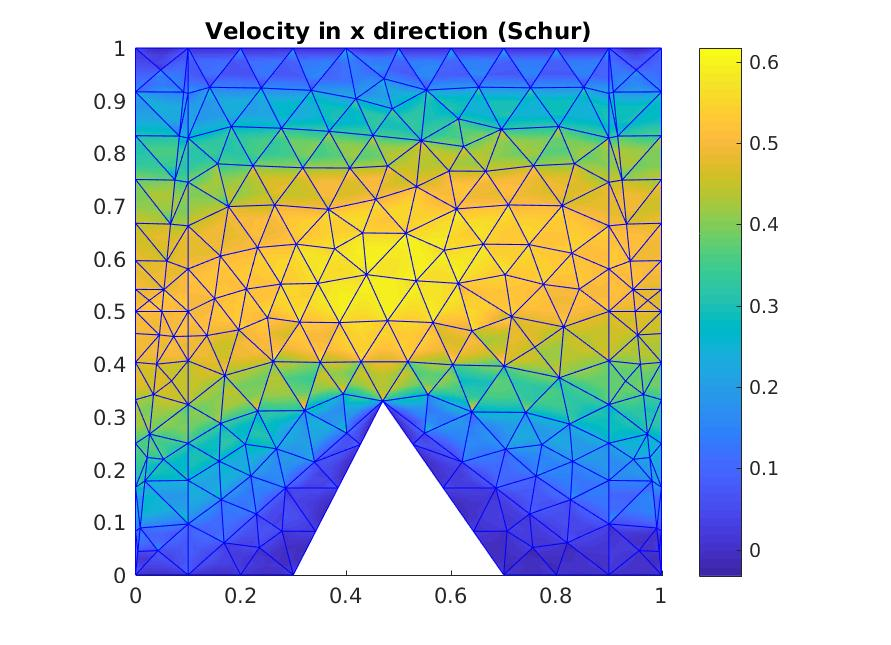
\includegraphics[width=\linewidth]{offline_velocity_1_at_47_33.jpg}
\caption{Velocity $x-$direction DG solution} \label{vel_x_dg}
\end{subfigure}\hspace*{\fill}
\begin{subfigure}{0.31\textwidth}
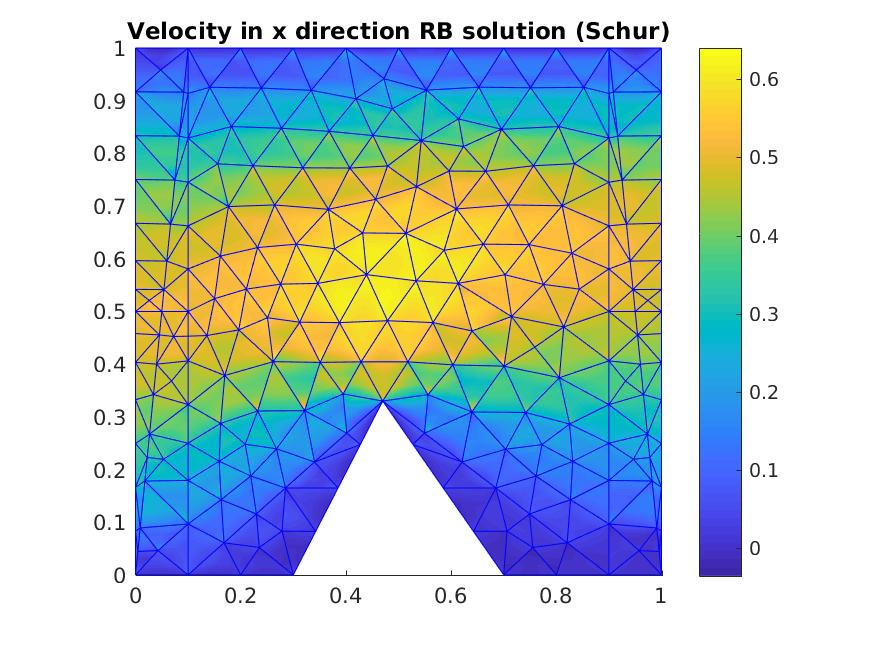
\includegraphics[width=\linewidth]{online_velocity_1_at_47_33.jpg}
\caption{Velocity $x-$direction RB solution} \label{vel_x_rb}
\end{subfigure}
\begin{subfigure}{0.31\textwidth}
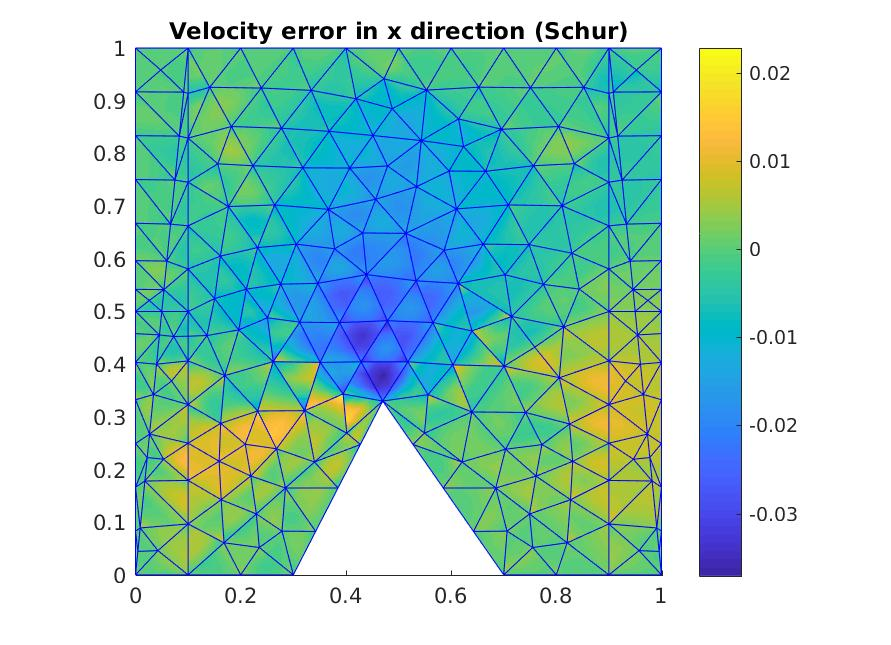
\includegraphics[width=\linewidth]{velocity_error_1_at_47_33.jpg}
\caption{$x-$component of Velocity absolute error $\overrightarrow{u}-\overrightarrow{u}_N$} \label{error_x_vel}
\end{subfigure}

\begin{subfigure}{0.31\textwidth}
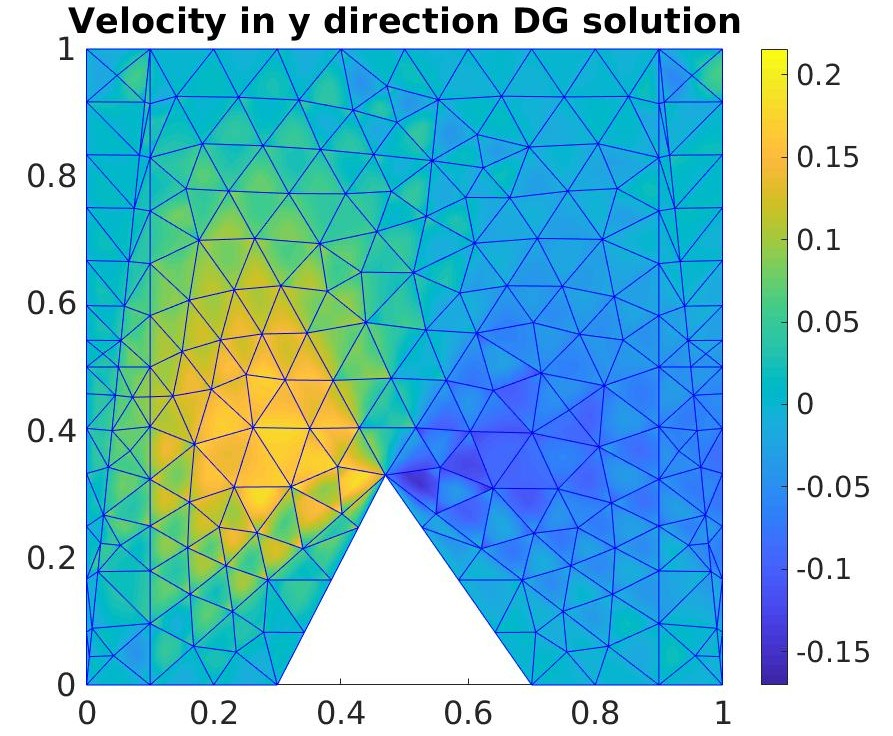
\includegraphics[width=\linewidth]{offline_velocity_2_at_47_33.jpg}
\caption{Velocity $y-$direction DG solution} \label{vel_y_dg}
\end{subfigure}\hspace*{\fill}
\begin{subfigure}{0.31\textwidth}
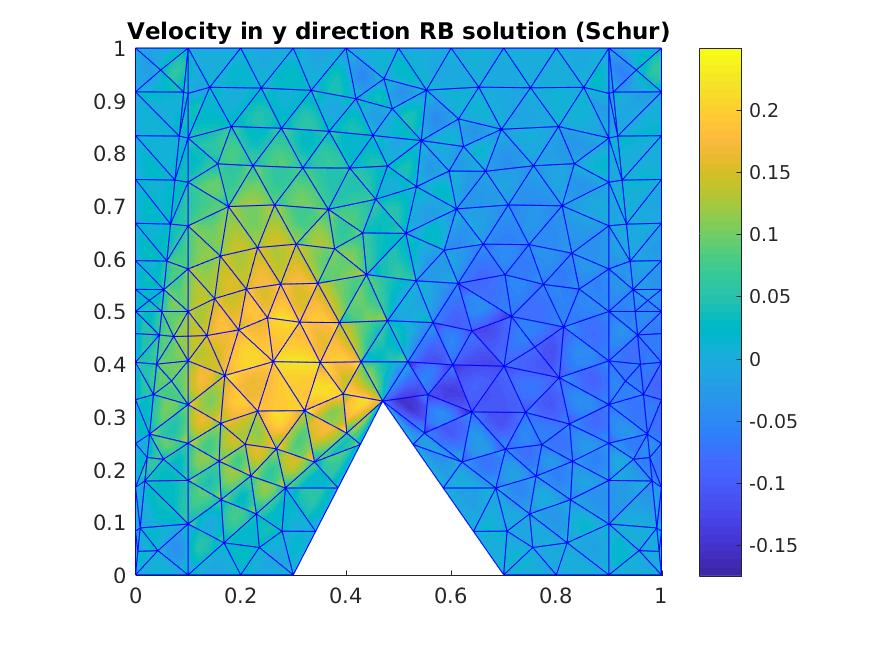
\includegraphics[width=\linewidth]{online_velocity_2_at_47_33.jpg}
\caption{Velocity $y-$direction RB solution} \label{vel_y_rb}
\end{subfigure}
\begin{subfigure}{0.31\textwidth}
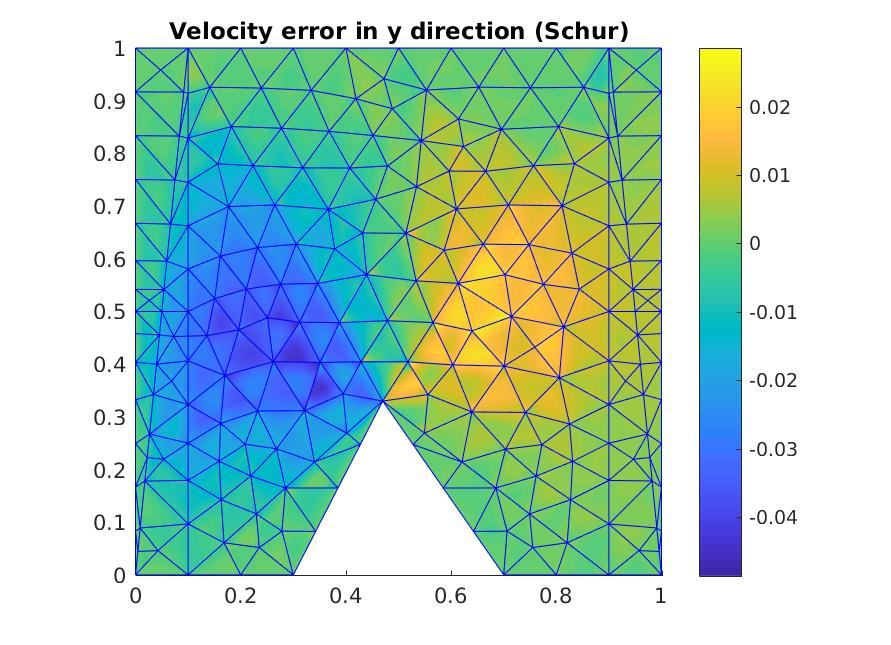
\includegraphics[width=\linewidth]{velocity_error_2_at_47_33.jpg}
\caption{$y-$component of Velocity absolute error $\overrightarrow{u}-\overrightarrow{u}_N$} \label{error_y_vel}
\end{subfigure}

\begin{subfigure}{0.31\textwidth}
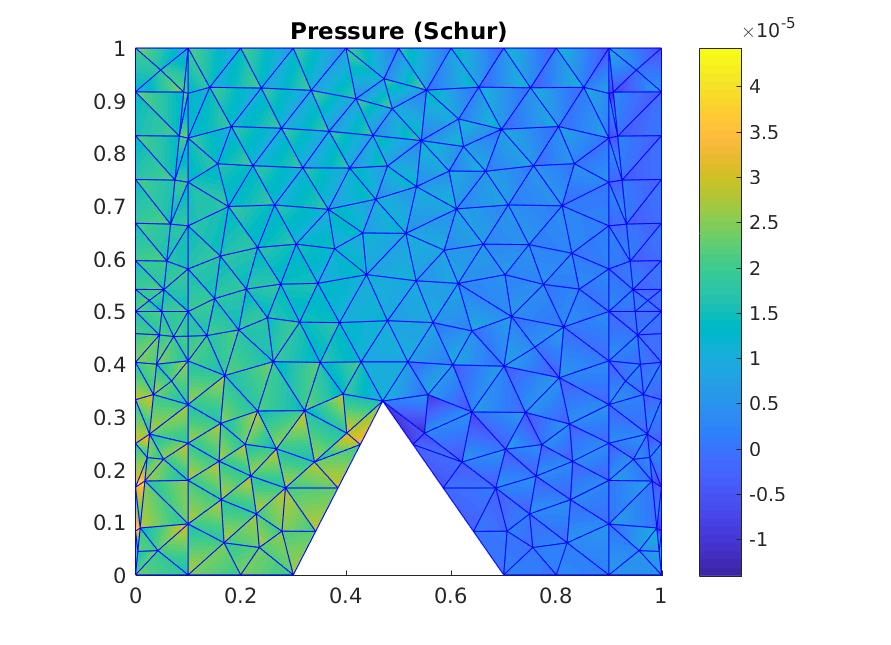
\includegraphics[width=\linewidth]{offline_pressure_at_47_33.jpg}
\caption{Pressure DG solution} \label{pre_dg}
\end{subfigure}\hspace*{\fill}
\begin{subfigure}{0.31\textwidth}
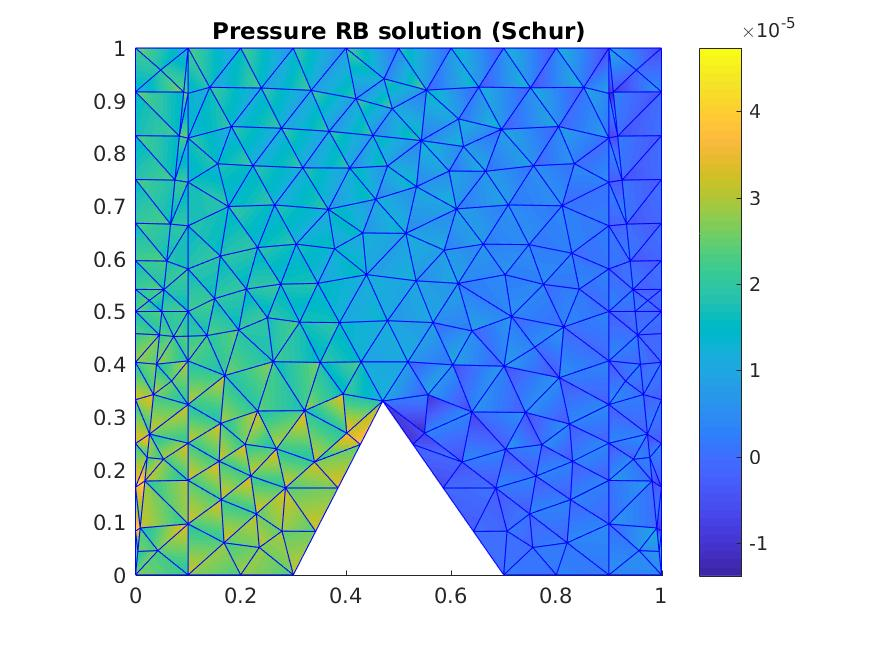
\includegraphics[width=\linewidth]{online_pressure_at_47_33.jpg}
\caption{Pressure RB solution} \label{pre_rb}
\end{subfigure}
\begin{subfigure}{0.31\textwidth}
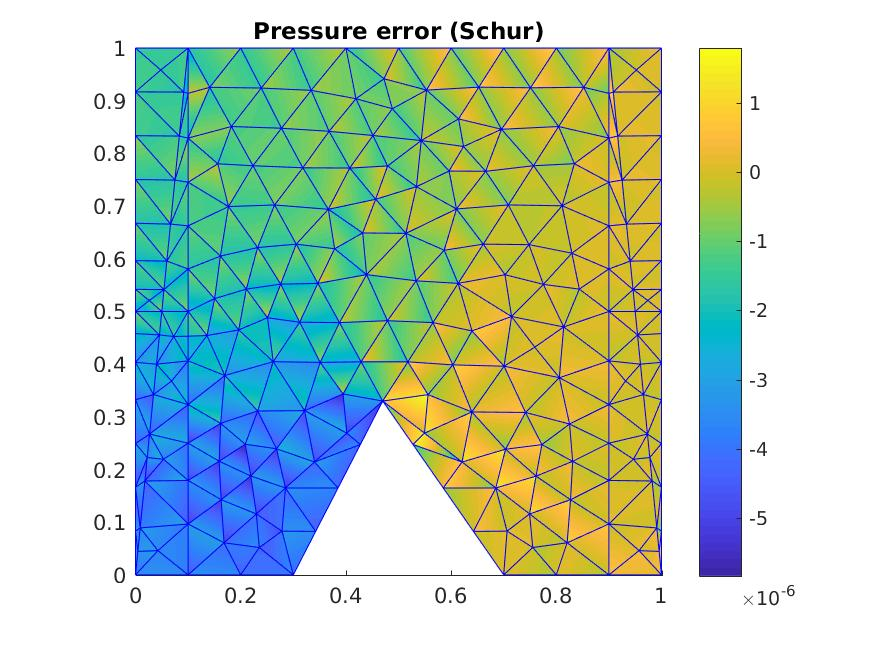
\includegraphics[width=\linewidth]{pressure_error_at_47_33.jpg}
\caption{Pressure absolute error $p-p_N$} \label{pre_error}
\end{subfigure}
\caption{DG and RB solution $[\mu_x \ \mu_y] = [0.47 \ 0.33]$} 
\label{dg_rb_solution_47_33}
\end{figure}

\begin{figure}
\begin{subfigure}{0.48\textwidth}
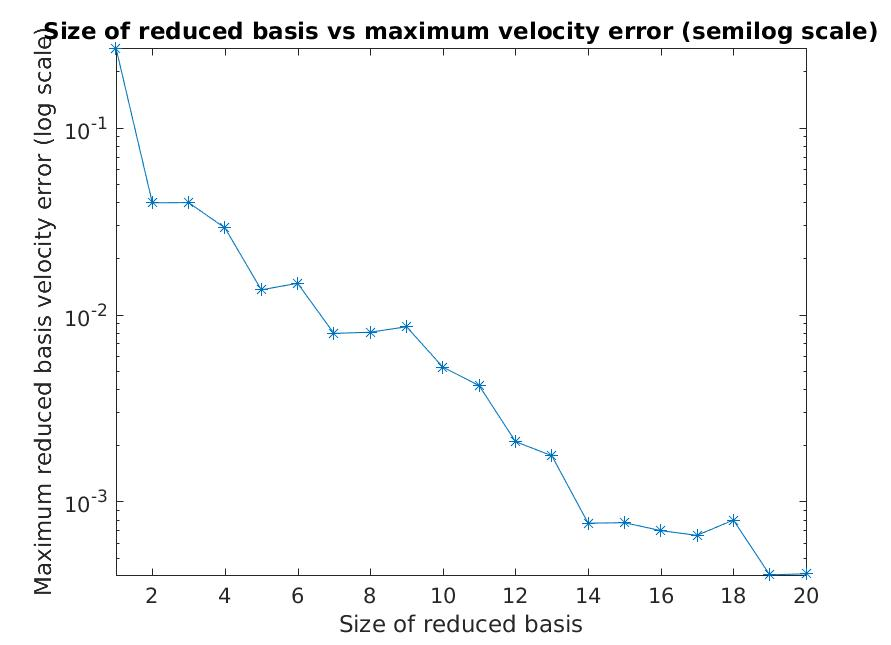
\includegraphics[width=\linewidth]{size_vs_maximum_reduced_basis_velocity_error_semilog.jpg}
\caption{Size of reduced basis space vs. Maximum relative error in velocity with inner product induced by $\bm{M}_v$} \label{error_vs_basis_velocity}
\end{subfigure}\hspace*{\fill}
\begin{subfigure}{0.48\textwidth}
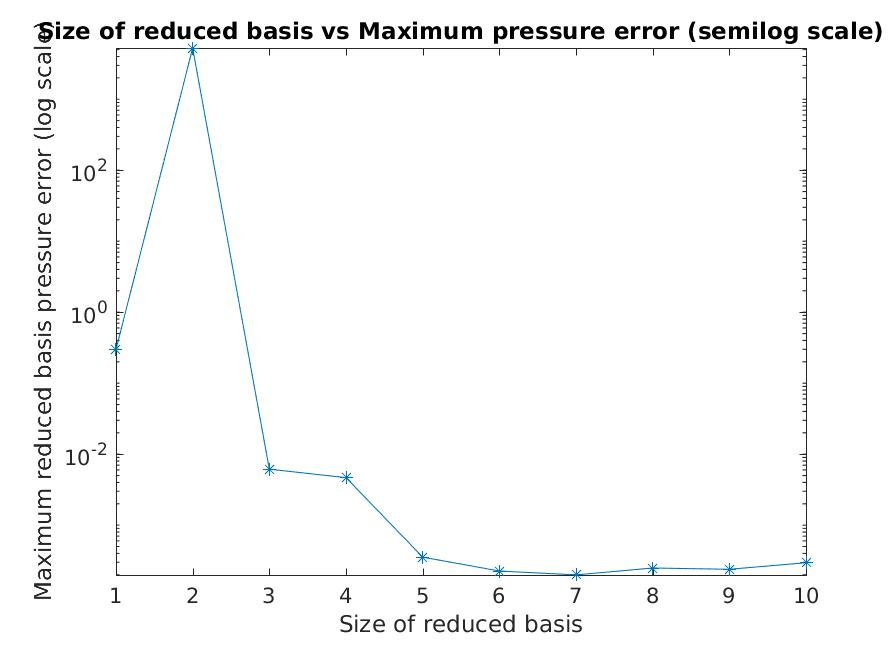
\includegraphics[width=\linewidth]{size_vs_maximum_reduced_basis_pressure_error_semilog.jpg}
\caption{Size of reduced basis space vs. Maximum relative error in pressure with inner product induced by $\bm{M}_p$} \label{error_vs_basis_pressure}
\end{subfigure}
  \caption{Size of reduced basis vs Maximum relative error} 
\label{error_vs_basis}
\end{figure}

\begin{figure}
\begin{subfigure}{0.48\textwidth}
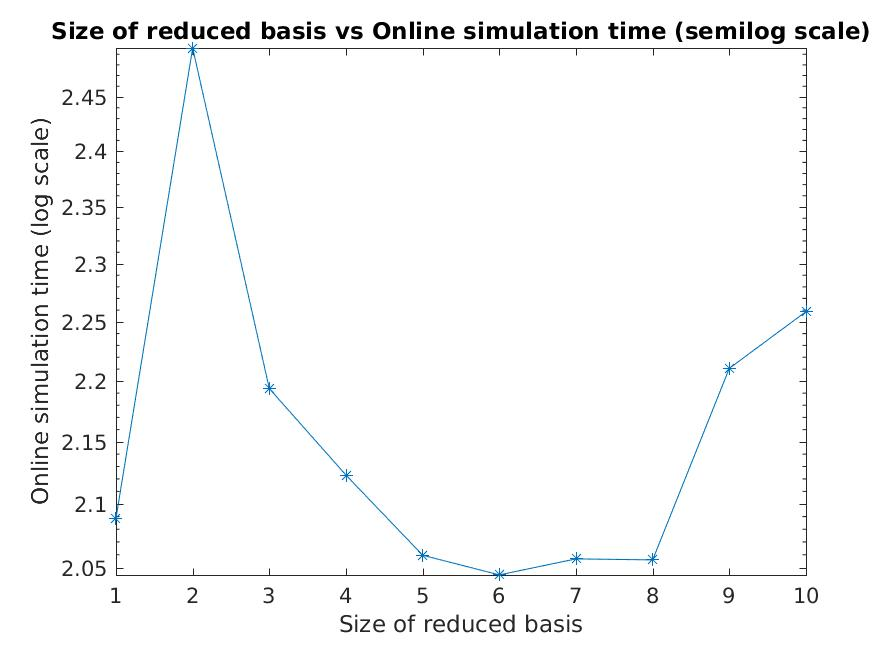
\includegraphics[width=\linewidth]{size_vs_online_simulation_time_semilog.jpg}
\caption{Size of reduced basis vs Online simulation time (semilog scale)} \label{online_simulation_time_vs_basis}
\end{subfigure}\hspace*{\fill}
\begin{subfigure}{0.48\textwidth}
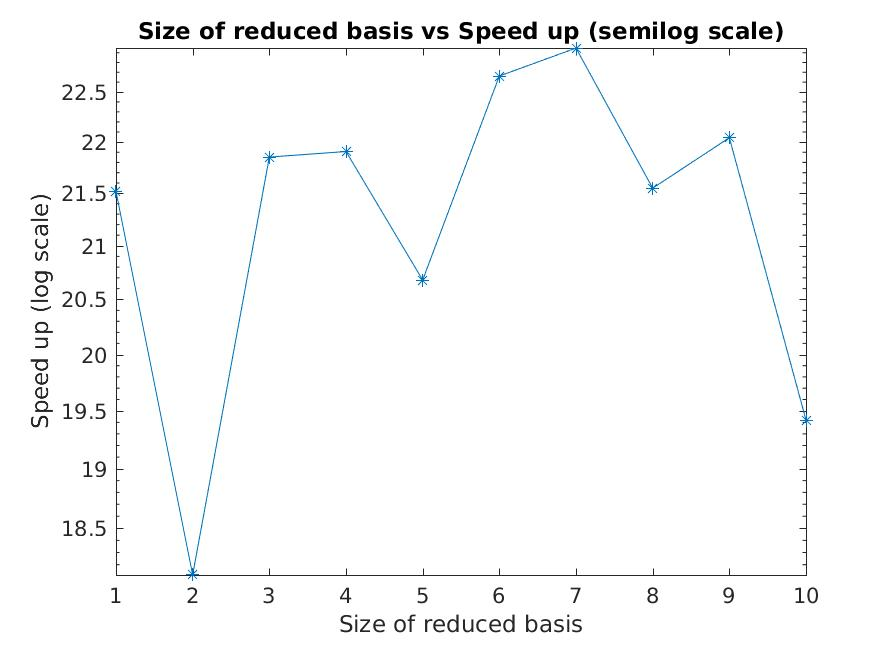
\includegraphics[width=\linewidth]{size_vs_reduced_basis_semilog.jpg}
\caption{Size of reduced basis vs Speed up (semilog scale)} \label{time_vs_speedup}
\end{subfigure}
\caption{Size of reduced basis for velocity vs Online computational time} 
\label{basis_vs_time}
\end{figure}

\bibliographystyle{spbasic.bst}
\bibliography{references.tex}
%%%%%%%%%%%%%%%%%%%% author.tex %%%%%%%%%%%%%%%%%%%%%%%%%%%%%%%%%%%
%
% sample root file for your "contribution" to a contributed volume
%
% Use this file as a template for your own input.
%
%%%%%%%%%%%%%%%% Springer %%%%%%%%%%%%%%%%%%%%%%%%%%%%%%%%%%


% RECOMMENDED %%%%%%%%%%%%%%%%%%%%%%%%%%%%%%%%%%%%%%%%%%%%%%%%%%%
\documentclass[graybox]{svmult}

% choose options for [] as required from the list
% in the Reference Guide

\usepackage{type1cm}        % activate if the above 3 fonts are
                            % not available on your system
%
\usepackage{makeidx}         % allows index generation
\usepackage{graphicx}        % standard LaTeX graphics tool
                             % when including figure files
\usepackage{multicol}        % used for the two-column index
\usepackage[bottom]{footmisc}% places footnotes at page bottom


\usepackage{newtxtext}       % 
\usepackage{newtxmath}       % selects Times Roman as basic font

\usepackage{url}

%%Nirav added
\newenvironment{spmatrix}[1]
 {\def\mysubscript{#1}\mathop\bgroup\begin{pmatrix}}
 {\end{pmatrix}\egroup_{\textstyle\mathstrut\mysubscript}}
\DeclareMathOperator{\Tr}{Tr}
\DeclareMathOperator{\spn}{span}
\usepackage{bm}
\usepackage{tikz}
\usepackage{wrapfig}
\usepackage[export]{adjustbox}
\usepackage{subcaption}
\usepackage{natbib}
\captionsetup{compatibility=false}
%%Nirav added over

% see the list of further useful packages
% in the Reference Guide

\makeindex             % used for the subject index
                       % please use the style svind.ist with
                       % your makeindex program

%%%%%%%%%%%%%%%%%%%%%%%%%%%%%%%%%%%%%%%%%%%%%%%%%%%%%%%%%%%%%%%%%%%%%%%%%%%%%%%%%%%%%%%%%

\begin{document}

\title{Discontinuous Galerkin model order reduction of geometrically parametrized Stokes flow}
% Use \titlerunning{Short Title} for an abbreviated version of
% your contribution title if the original one is too long
\author{Nirav Vasant Shah, Martin Hess and Gianluigi Rozza}
% Use \authorrunning{Short Title} for an abbreviated version of
% your contribution title if the original one is too long
\institute{Nirav Vasant Shah \at Scuola Internazionale Superiore di Studi Avanzati - via Bonomea, 265 - 34136 Trieste ITALY, \email{snirav@sissa.it}
\and Martin Hess \at Scuola Internazionale Superiore di Studi Avanzati - via Bonomea, 265 - 34136 Trieste ITALY \email{martin.hess@sissa.it}}
%
% Use the package "url.sty" to avoid
% problems with special characters
% used in your e-mail or web address
%
\maketitle

\abstract*{Each chapter should be preceded by an abstract (no more than 200 words) that summarizes the content. The abstract will appear \textit{online} at \url{www.SpringerLink.com} and be available with unrestricted access. This allows unregistered users to read the abstract as a teaser for the complete chapter.
Please use the 'starred' version of the \texttt{abstract} command for typesetting the text of the online abstracts (cf. source file of this chapter template \texttt{abstract}) and include them with the source files of your manuscript. Use the plain \texttt{abstract} command if the abstract is also to appear in the printed version of the book.}

\abstract{The present work focuses on geometrical parametrization and reduced order modeling of Stokes flow. We discuss the concept of geometric parametrization and its application along with importance of reduced order model technique.  The full order model is based on discontinuous Galerkin method interior penalty formulation. We introduce broken Sobolev spaces, relevant norms, jump and mean operator, weak formulation. The operators are transformed from fixed domain to parameter dependent domain by exploring affine parameter dependence. Proper orthogonal decomposition is applied to geometrically parametrized Stokes flow to obtain basis of function space for reduced order model. By using Galerkin projection the linear system is projected onto reduced space. During the process, offline-online decomposition is used to separate parameter independent and parameter independent operations. Finally the technique is applied to a test problem. The numerical outcomes presented include the experimental error analysis and measurement of online simulation time. \cite{psysoc-journal}\\
\textbf{Keywords:} Discontinuous Galerkin method, Stokes flow, Geometric parametrization, Proper orthogonal decomposition }

\section{Introduction}
\label{introduction}

The subject of mathematical applications in fluid mechanics starts with one of the variants of the Navier-Stokes equations, such as the Stokes equation. Almost all processes of fluid mechanics require considerations related to the Navier-Stokes equations. Navier-Stokes equation is non-linear, characterizing flow fluctuations. However, in case of laminar flow, i.e. when fluctuations are negligible, this linearized form of the Navier-Stokes equation is the Stokes equation.

Discontinuous Galerkin method (DGM) has found traction as numerical method for elliptic problems \textbf{pereire reference} as well as hyperbolic problems \textbf{Book on compressible flow reference}. This is due to its several advantages over Finite Element Method (FEM) and Finite Volume Method (FVM). In fact, DGM is considered as combination of FEM and FVM. DGM uses polynomial approximation of suitable degree providing higher accuracy as well as allows discontinuity at the interface, by the concept of numerical flux, allowing greater flexibility. This fact makes DGM naturally attractive to problems, such as shock capturing, due to presence of steep gradients or discontinuities. Additionally, since the Dirichlet conditions are applied as boundary penalty, it avoids necessity to work with subspace of Sobolev space such as in case of FEM. Several variants of DGM exist based on computational advantages such as sparsity pattern or extension of computational stencil, complexity of numerical implementation etc.

Geometric parametrization has emerged as important application of Parametric Partial Differential Equations (PPDEs) and as alternative to shape optimization. The concept of geometric parametrization allows to transfer operator evaluated on one geometric domain to another geometric domain efficiently. For linear equations, this means exploiting affine parameter dependence as will be shown in later section. Model Order Reduction (MOR) on the other hand allows reducing the size of the system to be solved and working with the smaller system containing only dominant components and discarding the non-dominant components. It is pertinent to mention that identifying "dominant" components is critical to the success of model order reduction strategy. Optimization of engineering components using geometric parametrization combined with MOR for PPDEs has given quite useful results in the fields such as mechanical, naval and aeronautic designs. Also, the  faster computations obtained by MOR has helped in many query context, real time computation and quick transfer of computational results to industrial problems.

In the present work, we first introduce notion of parametrization characterizing geometry of the domain under consideration. We subsequently introduce Discontinuous Galerkin Interior Penalty Method (DG-IPM) for stokes flow. We then explain exploiting affine parameter dependence and its application in the context of offline-online decomposition. We then apply Proper Orthogonal Decomposition (POD) for constructing reduced basis space and apply Galerkin projection to project the system of equations on the space constructed by POD. Finally we present a test problem to demonstrate the introduced method and numerical result.

\section{Geometric parametrization}\label{geometric_parametrization_section}

Consider domain $\Omega = \Omega(\mu) \in \mathbb{R}^d$ as open bounded domain. The parameter set $\mu \in \mathbb{P}$, where $\mathbb{P}$ is parameter space, completely characterizes the domain. Also, consider a parameter set $\bar{\mu} \in \mathbb{P}$, as the known parameter set and $\Omega(\bar{\mu})$ as the reference domain, whose configuration is completely known. The mapping $\bm{F}(\cdot,\mu) : \Omega(\bar{\mu}) \rightarrow \Omega(\mu)$ links reference domain and parametrized domain. Divide the domain $\Omega(\mu)$ into $n_{su}$ subdomains such that $\Omega(\mu) = \bigcup\limits_{i=1}^{n_{su}} \Omega_i(\mu) \ , \ \Omega_i(\mu) \bigcap \Omega_j(\mu) = \emptyset \ , \ \text{for} \ i \neq j$. The boundary of $\Omega(\mu)$, that is $\partial \Omega(\mu)$ is divided into Neumann boundary $\Gamma_N(\mu)$ and Dirichlet boundary $\Gamma_D(\mu)$ i.e. $\partial \Omega(\mu) = \Gamma_N(\mu) \cup \Gamma_D(\mu)$.

In the case of affine transformation, $\bm{F}$ is of the form,
\begin{gather}\label{affine_F}
x = \bm{F}(\hat{x},\mu) = \bm{G}_F(\mu)\hat{x} + c_F(\mu) \ ; \forall x \in \Omega \ , \ \hat{x} \in \Omega(\bar{\mu}) \ .
\end{gather}

The inverse map $\bm{T}$ is expressed in the form,
\begin{gather}\label{affine_T}
\hat{x} = \bm{T}(x,\mu) = \bm{G}_T(\mu)x + c_T(\mu) \ ; \forall x \in \Omega \ , \ \hat{x} \in \Omega(\bar{\mu}) \ .
\end{gather}

\section{Discontinuous Galerkin formulation}
\label{DG_formulation}

Each subdomain is divided into $N_{el}$ number of triangular elements $\tau_k$ such that $\Omega = \bigcup\limits_{k=1}^{N_{el}} \tau_k$. The triangulation $\mathcal{T}$ is the set of all triangular elements i.e. $\mathcal{T} = \lbrace \tau_k \rbrace_{k=1}^{N_{el}}$. The internal boundary $\Gamma = \lbrace \bigcup\limits_{k=1}^{N_{el} \partial \tau_k \rbrace} \backslash \partial \Omega$. The vertices of triangle ${\tau_k}_{k=1}^{N_{el}}$ are called nodes. $\overrightarrow{n}$ is the outward pointing normal to an edge of element.

The Stokes's equation in strong form can be stated as,
\begin{gather}\label{stokes_strong_form}
-\nu \Delta \overrightarrow{u} + \nabla p = \overrightarrow{f} \ , \ \text{in } \Omega \ , \\
\nabla \cdot \overrightarrow{u} = 0 \ , \ \text{in} \ \Omega \ , \\
\overrightarrow{u} = \overrightarrow{u}_D \ , \ \text{on } \Gamma_D \ , \\
-p \overrightarrow{n} + \nu \overrightarrow{n} \cdot \nabla \overrightarrow{u} = \overrightarrow{t} \ , \ \text{on} \ \Gamma_N \ .
\end{gather}

The velocity vector field $\overrightarrow{u}$ and pressure scalar field $p$ are the unknowns. $\nu$ is the material property known as kinematic viscosity. Vector $\overrightarrow{f}$ is external force term or source term. $\overrightarrow{u}_D$ is the Dirichlet velocity and $\overrightarrow{t}$ is the Neumann value.

Before introducing weak form let us introduce broken Sobolev spaces for variables.

The space for velocity is 
\begin{equation} \label{velocity_test}
\mathbb{V} = \lbrace \overrightarrow{\phi} \in (L^2(\Omega))^d | \ \overrightarrow{\phi} \in (P^D(\tau_k))^d \ , \ \tau_k \in \mathcal{T} \rbrace \ .
\end{equation}
The space for pressure is 
\begin{equation} \label{pressure_test}
\mathbb{Q} = \lbrace \psi \in (L^2(\Omega)) | \ \psi \in (P^{D-1}(\tau_k)) \ , \ \tau_k \in \mathcal{T} \rbrace \ .
\end{equation}
Here, $P^D(\tau_k)$ denotes space of polynomials of degree at most $D \geq 2$ over $\tau_k$.

The velocity $\overrightarrow{u}(x)$ and pressure $p(x)$ at any point $x \in \Omega$ is given by,
\begin{equation}\label{velocity_pressure_coefficients}
\overrightarrow{u}(x) = \sum\limits_{i=1}^{\overrightarrow{u}_{ndofs}} \overrightarrow{\phi}_i \hat{u}_i \ , \
p(x) = \sum\limits_{i=1}^{p_{ndofs}} \psi_i \hat{p}_i \ ,
\end{equation}
where $\hat{u}_i$'s and $\hat{p}_i$'s are coefficients of velocity basis functions and pressure basis functions respectively. 

\begin{figure}
\centering
\sidecaption[t]
\begin{tikzpicture}
\draw (0,0) node[anchor=north]{${}$}
  -- (4,0) node[anchor=north]{${}$}
  -- (0,4) node[anchor=south]{${}$}
  -- cycle;
\draw (4,4) node[anchor=north]{${}$}
  -- (4,0) node[anchor=north]{${}$}
  -- (0,4) node[anchor=south]{${}$}
  -- cycle;
\draw[->] (2,2)--(2.5,2.5)node[label={[xshift=0.4cm, yshift=-0.7cm]${\overrightarrow{n}^-}$}]{};
\draw[->] (2,2)--(1.5,1.5)node[label={[xshift=0cm, yshift=0cm]${\overrightarrow{n}^+}$}]{};
\node at (1,1){$\tau_{k}^-$};
\node at (3,3){$\tau_{k}^+$};
\node at (1.7,3){$\overrightarrow{\phi}^+,\psi^+$};
\node at (2.3,1){$\overrightarrow{\phi}^-,\psi^-$};
\end{tikzpicture}
\caption{Definition of jump and mean operator. \newline The superscript $+$ refers to quantity in the element itself and the superscript $-$ refers to quantity in the neighboring element}
\label{fig:Self_neighbour}
\end{figure}

In the subsequent sections $\left( \cdot \right),\left( \cdot \right)_{\Gamma_D},\left( \cdot \right)_{\Gamma_N},\left( \cdot \right)_{\Gamma}$ represent the $L^2$ scalar product over $\Omega,\Gamma_D,\Gamma_N,\Gamma$ respectively. The jump operator $\left[ \cdot \right]$ and the average operator $\lbrace \cdot \rbrace$ are are important concepts in DGM formulation and are required to approximate the numerical flux (Figure \ref{fig:Self_neighbour}).

The presence of normal vector $\overrightarrow{n}$ in jump and average operator introduced below allows symmetric formulation and also ensures that jump of a vector is vector and jump of a scalar is scalar.

\begin{itemize}
\item For vector quantity $\overrightarrow{\phi}$:
\begin{itemize}
\item Jump operator: 
$\left[\overrightarrow{\phi} \cdot \overrightarrow{n}\right] = \overrightarrow{\phi}^+ \cdot \overrightarrow{n}^+ + \overrightarrow{\phi}^- \cdot \overrightarrow{n}^-$ on $\Gamma$, $\left[\overrightarrow{\phi} \cdot \overrightarrow{n}\right] = \overrightarrow{\phi} \cdot \overrightarrow{n}$ on $\partial \Omega$.
\item Average operator:
$\lbrace \overrightarrow{\phi} \rbrace = \frac{\overrightarrow{\phi}^+ + \overrightarrow{\phi}^-}{2}$ on $\Gamma$, $\lbrace \overrightarrow{\phi} \rbrace = \overrightarrow{\phi}$ on $\partial \Omega$.
\end{itemize}
\item For scalar quantity $\psi$:
\begin{itemize}
\item Jump operator:
$\left[\psi \overrightarrow{n} \right] = \psi^+ \overrightarrow{n}^+ + \psi^- \overrightarrow{n}^-$ on $\Gamma$, $\left[\psi \overrightarrow{n} \right] = \psi \overrightarrow{n}$ on $\partial \Omega$.
\item Average operator:
$\lbrace \psi \rbrace = \frac{\psi^+ + \psi^-}{2}$ on $\Gamma$, $\lbrace \psi \rbrace = \psi$ on $\partial \Omega$. 
\end{itemize}
\end{itemize}

The weak form of Stokes equation is as follow,
\begin{gather}\label{stokes_weak_ch3}
a_{IP}(\overrightarrow{u},\overrightarrow{\phi}) + b(\overrightarrow{\phi},p) + \left( \lbrace p \rbrace,[\overrightarrow{n} \cdot \overrightarrow{\phi}] \right)_{\Gamma \cup \Gamma_D} = l_{IP}(\overrightarrow{\phi}) \ , \\
a_{IP}(\overrightarrow{u},\overrightarrow{\phi}) = \left( \nabla \overrightarrow{u}, \nabla \overrightarrow{\phi} \right) + C_{11} \left( [\overrightarrow{u}],[\overrightarrow{\phi}] \right)_{\Gamma \cup \Gamma_D} - \nu \left( \lbrace \nabla \overrightarrow{u}\rbrace ,[\overrightarrow{n} \otimes \overrightarrow{\phi}] \right)_{\Gamma \cup \Gamma_D} - \nu \left( [\overrightarrow{n} \otimes \overrightarrow{u}], \lbrace \nabla \overrightarrow{\phi} \rbrace \right)_{\Gamma \cup \Gamma_D} \ , \\
b(\phi,\psi) = -\int_{\mathcal{T}} \psi \nabla \cdot \overrightarrow{\phi} \ , \\
l_{IP}(\overrightarrow{\phi}) = \left( \overrightarrow{f},\overrightarrow{\phi} \right) + \left( \overrightarrow{t},\overrightarrow{\phi} \right)_{\Gamma_N} + C_{11} \left(\overrightarrow{u}_D,\overrightarrow{\phi}\right)_{\Gamma_D} - \left( \overrightarrow{n} \otimes \overrightarrow{u}_D, \nu \nabla \overrightarrow{\phi} \right)_{\Gamma_D} \ .
\end{gather}

The penalty parameter $C_{11}>0$ in $a_{IP}(\overrightarrow{u},\overrightarrow{\phi})$ is an empirical constant to be kept large enough to maintain coercivity of bilinear form.

The weak for of continuity equation is as follow,
\begin{equation}\label{contiuity_weak_ch3}
\begin{split}
b(\overrightarrow{u},\psi) + ({\psi},[\overrightarrow{n} \cdot \overrightarrow{u}])_{\Gamma \cup \Gamma_D} = (\psi,\overrightarrow{n} \cdot \overrightarrow{u}_D)_{\Gamma_D} \ .
\end{split}
\end{equation}

In discrete form system of equations can be written as, 
\begin{equation} \label{Stokes_matrix_ch3}
\begin{spmatrix}{\textrm{Stiffness matrix}}
    \bm{A} & \bm{B} \\
    \bm{B}^T & 0
\end{spmatrix}
\begin{spmatrix}{\textrm{Solution vector}}
    U \\
    P
\end{spmatrix}
=
\begin{spmatrix}{\textrm{Right hand side (Known)}}
    F_1  \\
    F_2
\end{spmatrix}
\textrm{.}
\end{equation}

Here, $\bm{A}_{ij} = a_{IP} (\overrightarrow{\phi}_i,\overrightarrow{\phi}_j)$, $\bm{B}_{ij} = b(\overrightarrow{\phi}_i,\psi_j) + \left( \lbrace \psi_j \rbrace , [n \cdot \phi_i]\right)_{\Gamma \cup \Gamma_D}$, $F_1 = l_{IP}(\overrightarrow{\phi}_i)$ and $F_2 = \left( \psi_j,\overrightarrow{n} \cdot \overrightarrow{u}_D \right)_{\Gamma_D}$. The column vectors $U$ and $P$ are coefficients $\hat{u}$'s and $\hat{p}$'s from equation \eqref{velocity_pressure_coefficients}.

\section{Affine expansion}

We evaluate and solve the Stokes equation weak formulation on reference domain $\Omega{\bar{\mu}}$. Given a parameter set $\mu \neq \bar{\mu}$ we need to evaluate the linear systems of equation \eqref{Stokes_matrix_ch3} on new domain $\Omega(\mu)$. To accomplish this we use affine expansion using linear nature of equation and diving $\Omega(\bar{\mu})$ into triangular subdomains $\Omega_i(\bar{\mu}) \ , \ i = \lbrace 1,2,\ldots,n_{su} \rbrace$ as explained earlier in the section geometric parametrization [Section \ref{geometric_parametrization_section}]. The affine expansion of operators is essentially change of variable and has been explained in literatures such as \textbf{ADD affine expansion literature}. However it is pertinent to mention two expansions as specific to DGM formulation will be mentioned here as below.

\begin{itemize}
\item In order to transfer the terms containing jump and average operator following approach is used in present analysis.
\begin{equation*}\label{jump_average_term_split}
\begin{split}
\left(\lbrace \nabla \overrightarrow{\phi} \rbrace , \left[ \overrightarrow{n} \otimes \overrightarrow{\phi}  \right]  \right) = \left( \nabla \overrightarrow{\phi}^+ , \overrightarrow{n}^+ \otimes \overrightarrow{\phi}^+ \right) + \left( \nabla \overrightarrow{\phi}^+ , \overrightarrow{n}^- \otimes \overrightarrow{\phi}^- \right) + \\ 
\left( \nabla \overrightarrow{\phi}^- , \overrightarrow{n}^+ \otimes \overrightarrow{\phi}^+ \right) + \left( \nabla \overrightarrow{\phi}^- , \overrightarrow{n}^- \otimes \overrightarrow{\phi}^- \right) \ .
\end{split}
\end{equation*}
Each term on right hand side of equation \eqref{jump_average_term_split} can now be transformed using affine map.

\item The coercivity term $C_{11}\left( [\overrightarrow{\phi}],[\overrightarrow{u}] \right)_{\Gamma \cup \Gamma_D}$ is not transformed but used as evaluated on reference domain $\Omega(\bar{\mu})$. The affine transformation is given by,
\begin{equation*}
\begin{split}
C_{11}\left( [\overrightarrow{\phi}(\hat{x}),\overrightarrow{u}(\hat{x})] \right)_{\Gamma(\mu) \cup \Gamma_D(\mu)} = C_{11} \alpha \left( [\overrightarrow{\phi}(\bm{F}(\hat{x})),\overrightarrow{u}(\bm{F}(\hat{x}))] \right)_{\Gamma(\bar{\mu}) \cup \Gamma_D(\bar{\mu})} \ , \\
\alpha = \frac{meas\left( \Gamma(\mu) \cup \Gamma_D(\mu)\right)}{meas\left( \Gamma(\bar{\mu}) \cup \Gamma_D(\bar{\mu})\right)} \ , \ \hat{x} \in \Omega(\bar{\mu}) \ , \ x \in \Omega(\mu) \ .
\end{split}
\end{equation*}

Since, $C_{11}$ is empirical coefficient replacing $C_{11} \alpha$ with $C_{11}$ will not change the formulation as long as coercivity of $a_{IP}$ over parameter space $\mathbb{P}$ is maintained. In the present analysis, $C_{11}$ is not calculated exactly but only order of magnitude required for $C_{11}$ is estimated and $C_{11}$ is kept one magnitude larger as safeguard against round-off errors. As long as the domain $\Omega(\mu)$ is not deformed much compared to its reference configuration $\Omega(\bar{\mu})$, $C_{11}$ and $C_{11}\alpha$ will have the same order of magnitude. However, regardless of this fact, large deformations are not favorable as it will lead to bad mesh quality and in turn, will lead to poor DGM-approximation.
\end{itemize}

\section{Reduced basis method}

\subsection{Snapshot proper orthogonal decomposition}\label{POD_section}

We present now snapshot proper orthogonal decomposition method. Here, ``snapshot" means solution calculated by discontinuous Galerkin method. We calculate solution based on $\mu_n, n \in \lbrace 1,....,n_s \rbrace$ i.e. $n_s$ snapshots are generated. We also introduce inner product matrices $\bm{M}_v \in \mathbb{R}^{\overrightarrow{u}_{ndofs} \times \overrightarrow{u}_{ndofs}}$ and $\bm{M}_p \in \mathbb{R}^{p_{ndofs} \times p_{ndofs}}$.

\begin{gather*}
\bm{M}_v = \int_{\Omega} \overrightarrow{\phi}_i \cdot \overrightarrow{\phi}_j + \sum_{k=1}^{N_{el}} \int_{\tau_k} \nabla \overrightarrow{\phi}_i : \nabla \overrightarrow{\phi}_j \ , \ i,j = 1, \ldots, \overrightarrow{u}_{ndofs} \ , \\
\bm{M}_p = \int_{\Omega} \psi_i \psi_j \ , \ i,j = 1, \ldots, p_{ndofs} \ .
\end{gather*}

We also introduce matrices storing velocity snapshots $\bm{S}_v$ and storing pressure snapshots $\bm{S}_p$. We discuss the method only for velocity snapshots. The method is similar for pressure snapshots. We note the size of matrices, useful for matrix operations presented hereafter.

\begin{gather*}
\bm{S}_v \in \mathbb{R}^{\overrightarrow{u}_{ndofs} \times n_s} \ , \ \bm{S}_p \in \mathbb{R}^{p_{ndofs} \times n_s} \ , \\
\bm{M}_v \in \mathbb{R}^{\overrightarrow{u}_{ndofs} \times \overrightarrow{u}_{ndofs}} \ ,\ \bm{M}_p \in \mathbb{R}^{p_{ndofs} \times p_{ndofs}} \ .
\end{gather*}

\subsection{Spectral decomposition of snapshots}\label{spectral_decomposition_section}

We denote the dimension of reduced basis as $N$ and assert that $N << n_s$. We now perform the spectral decomposition of $\bm{S}_v^T \bm{M}_v \bm{S}_v$,

\begin{equation}\label{snapshot_eigen_value}
\bm{S}_v^T \bm{M}_v \bm{S}_v = \bm{V} \bm{\Theta} \bm{V}^T \ .
\end{equation}

The columns of $V$ are eigenvectors and $\Theta$ has eigenvalues $\theta_i \ , \ 1 \leq i \leq n_s$ such that,
\begin{equation}
\Theta_{ij} = \theta_i \delta_{ij} \ .
\end{equation}

We also note that $\theta_i > 0$ and $\theta_1 \geq \theta_2 \geq ... \geq \theta_{n_s}$ i.e. the eigenvalues are in sorted order. We form the reduced basis by linear combination of the snapshot vector,
\begin{equation}\label{linear_combination_snapshots}
\bm{B}_v = \bm{S}_v \bm{A} \ , \ \bm{A} \in \mathbb{R}^{n_s \times N} \ .
\end{equation}
the reduced basis for velocity basis function $\overrightarrow{\phi}_N$ is formed by,
\begin{equation}
\overrightarrow{\phi}_N = \overrightarrow{\phi}^T \bm{B}_v \ .
\end{equation}

Considering orthonormality of reduced basis $\overrightarrow{\phi}_N$ with respect to inner product induced by $\bm{M}_v$, from equation \eqref{snapshot_eigen_value},
\begin{equation}
<\overrightarrow{\phi}_N,\overrightarrow{\phi}_N>_{\bm{M}_v} = \bm{B}_v^T \bm{M}_v \bm{B}_v = I \ .
\end{equation}
From equation \eqref{linear_combination_snapshots}, we express matrix $\bm{A}$ as,
\begin{equation}
\bm{A} = \bm{V} \bm{\Theta}^{-\frac{1}{2}} \bm{R} \ , \ \bm{R} = [\bm{I}_{N \times N} ; \bm{0}_{(N-n_s \times N)}] \ \text{and accordingly} \ \bm{B}_v = \bm{S}_v \bm{V} \bm{\Theta}^{-\frac{1}{2}} \bm{R} \ .
\end{equation}
The columns of $\bm{B}_v$ now represent the basis functions for reduced space for velocity. Due to round-off errors, these basis functions may not be of unit magnitude and it is necessary to normalize the basis functions.

The reduced basis space $\bm{B}_p$ can be generated in similar manner using pressure snapshots $\bm{S}_p$ and inner product matrix $\bm{M}_p$.

\subsection{Galerkin reduced basis formulation}\label{Galerkin_section}

We now present the reduced bilinear form as,

\begin{equation} \label{stokes_equation_parameter}
a(u_N,\phi_N;\mu) + b(p_N,\phi_N;\mu) = f_1(\phi_N,\mu) \textrm{,}
\end{equation}

\begin{equation} \label{continuity_equation_parameter}
b(u_N,\psi_N;\mu) = f_2(\psi_N,\mu) \textrm{.}
\end{equation}

In discrete form, we form reduced equation as,

\begin{equation} \label{Stokes_matrix_reduced}
\begin{spmatrix}{\tilde{K}}
    \bm{B}_v^T \bm{A}(\mu) \bm{B}_v & \bm{B}_v^T \bm{B}(\mu) \bm{B}_v \\
    \bm{B}_p^T \bm{B}(\mu)^T \bm{B}_v & \bm{0}
\end{spmatrix}
\begin{spmatrix}{\zeta}
    U_N \\
    P_N
\end{spmatrix}
=
\begin{spmatrix}{\tilde{F}}
    \bm{B}_v^T F_1(\mu)  \\
    \bm{B}_p^T F_2(\mu)
\end{spmatrix} \ ,
\end{equation}
and accordingly we solve following variational form for reduced degrees of freedom $\zeta$,
\begin{equation}
\tilde{\bm{K}} \zeta = \tilde{F} \ ,
\end{equation}
and calculate reduced solutions $\overrightarrow{u}_N$ and $p_N$ as,
\begin{equation}
\overrightarrow{u}_N = \bm{B}_v U_N \ , \ p_N = \bm{B}_p P_N
\end{equation}

\section{Offline-online procedure}

The offline-online procedure is used to separate computationally intensive parameter independent offline procedure and faster parameter dependent online procedure \textbf{cite CRBM}. During the offline phase $n_s$ snapshots are computed and reduced basis spaces $\bm{B}_v$ and $\bm{B}_p$ are created. The offline procedure is outlined in section \ref{POD_section} and section \ref{spectral_decomposition_section}. During the online phase the systems of equations are projected on reduced space using Galerkin projection, the smaller systems of equation obtained by Galerkin projection is solved and the reduced basis solution is computed as outlined in section \ref{Galerkin_section}. The parameter dependent matrices in equation \eqref{Stokes_matrix_reduced} are evaluated by using affine decomposition.

\section{Numerical example}

We perform the POD-Galerkin method as mentioned in section \ref{POD_section} - section \ref{Galerkin_section}. The reference domain $\Omega{\bar{\mu}}$ is the unit square domain with triangle with vertices $(0.3,0),(0.5,0.3),(0.7,0)$ as obstacle. The geometric parameters are coordinates of tip of the obstacle i.e. $\bar{\mu} = (0.5,0.3)$. The boundary ${x=0}$ is Dirichlet boundary with inflow velocity at point $(0,y)$ as $u = (y(1-y), 0)$. The boundary ${x = 1}$ is a Neumann boundary with zero Neumann value i.e. $t = (0, 0)$. Other boundaries are Dirichlet boundary with no slip condition. The source term is $f = (0,0)$.

The training set was generated by random generation of $100$ parameters between the interval $[0.4,0.6] \times [0.4,0.6]$. The test set contained $10$ random parameters between the interval $[0.4,0.6] \times [0.4,0.6]$. For velocity basis function polynomial of degree $P^D = 2$ and for pressure basis function polynomial of degree $P^{D-1} = 1$ was used. The number of velocity degrees of freedom and pressure degrees of freedom were $\overrightarrow{u}_{ndofs} = 4704$ and $p_{ndofs} = 1176$ respectively.

Figure \ref{dg_rb_solution_47_33} shows solution computed by DGM and POD at parameter value $(0.47,33)$. Figure \ref{error_vs_basis} shows error vs size of reduced basis space. As can be seen the error drops with increasing size of basis function, however, this has to be at affordable cost of increased online simulation time (Figure \ref{basis_vs_time}).

\begin{figure}%[t!] % "[t!]" placement specifier just for this example
\begin{subfigure}{0.31\textwidth}
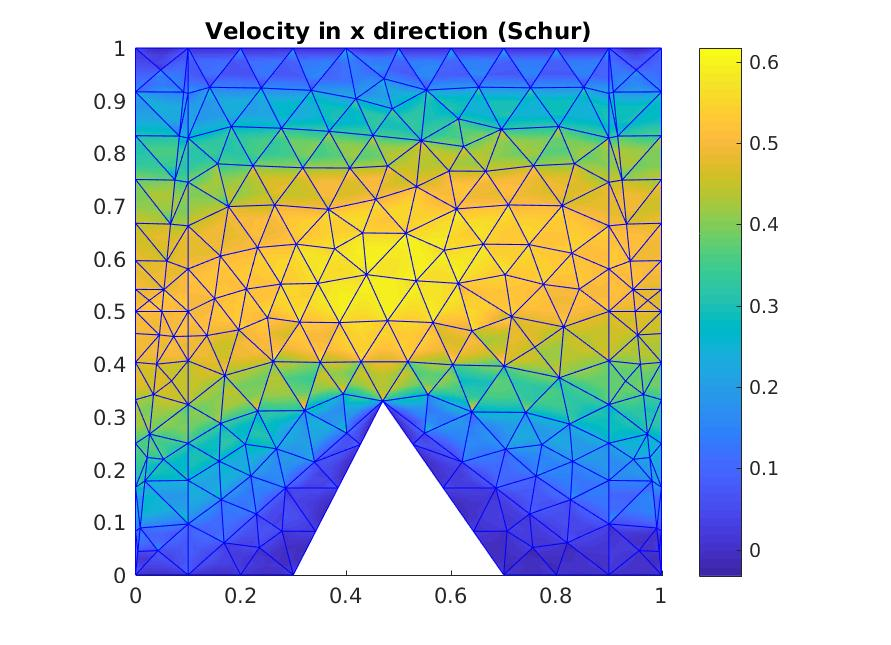
\includegraphics[width=\linewidth]{offline_velocity_1_at_47_33.jpg}
\caption{Velocity $x-$direction DG solution} \label{vel_x_dg}
\end{subfigure}\hspace*{\fill}
\begin{subfigure}{0.31\textwidth}
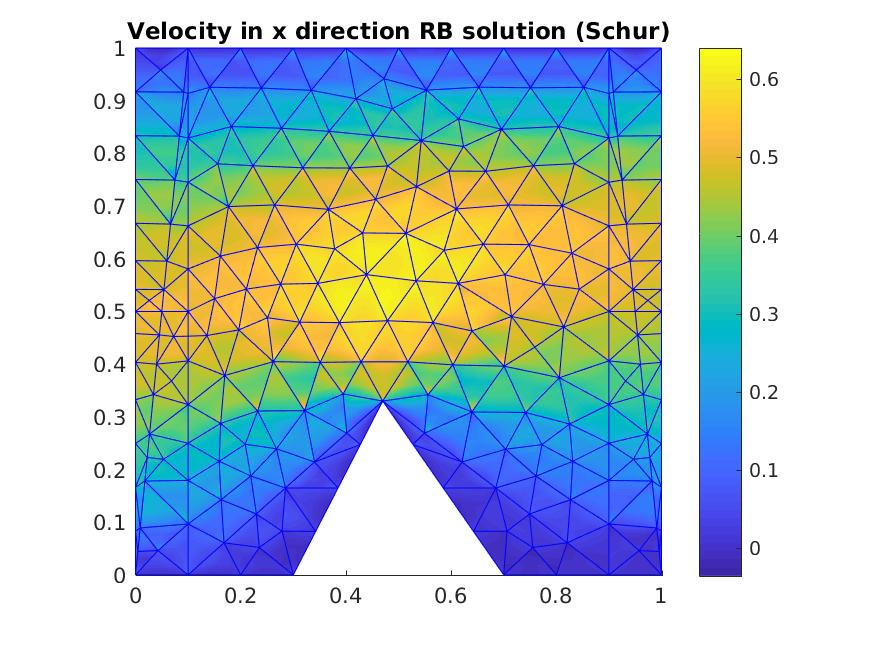
\includegraphics[width=\linewidth]{online_velocity_1_at_47_33.jpg}
\caption{Velocity $x-$direction RB solution} \label{vel_x_rb}
\end{subfigure}
\begin{subfigure}{0.31\textwidth}
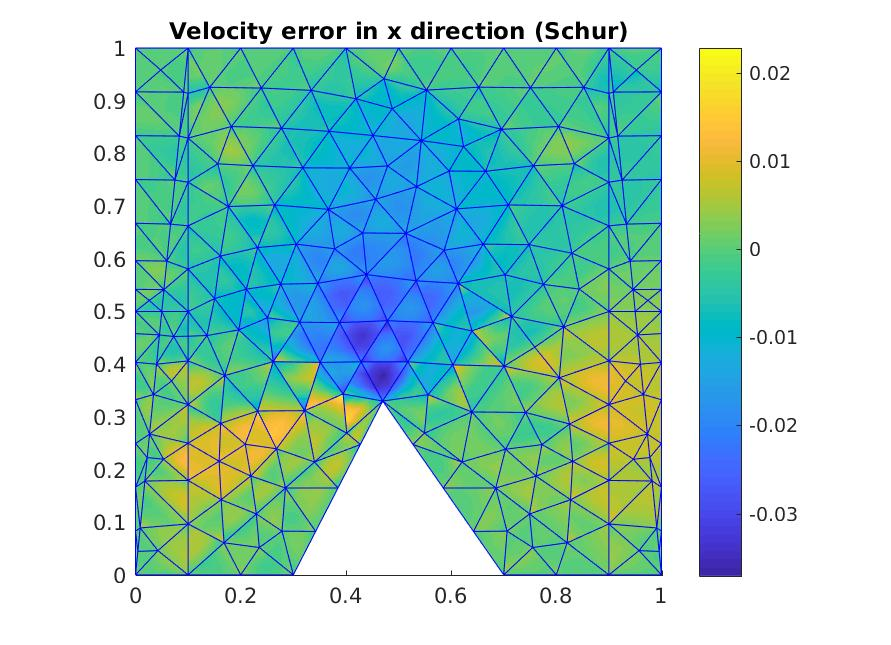
\includegraphics[width=\linewidth]{velocity_error_1_at_47_33.jpg}
\caption{$x-$component of Velocity absolute error $\overrightarrow{u}-\overrightarrow{u}_N$} \label{error_x_vel}
\end{subfigure}

\begin{subfigure}{0.31\textwidth}
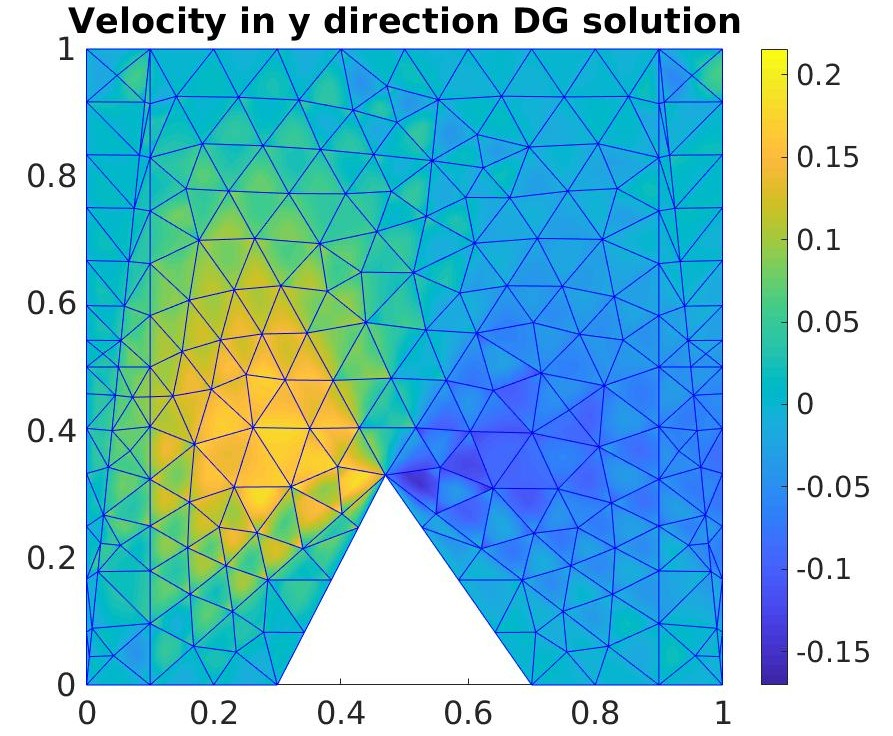
\includegraphics[width=\linewidth]{offline_velocity_2_at_47_33.jpg}
\caption{Velocity $y-$direction DG solution} \label{vel_y_dg}
\end{subfigure}\hspace*{\fill}
\begin{subfigure}{0.31\textwidth}
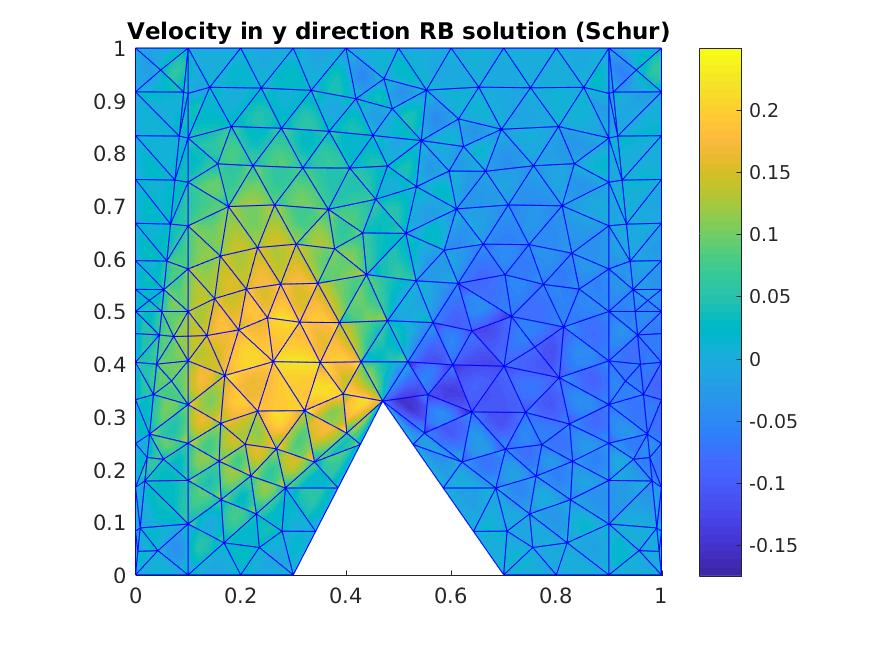
\includegraphics[width=\linewidth]{online_velocity_2_at_47_33.jpg}
\caption{Velocity $y-$direction RB solution} \label{vel_y_rb}
\end{subfigure}
\begin{subfigure}{0.31\textwidth}
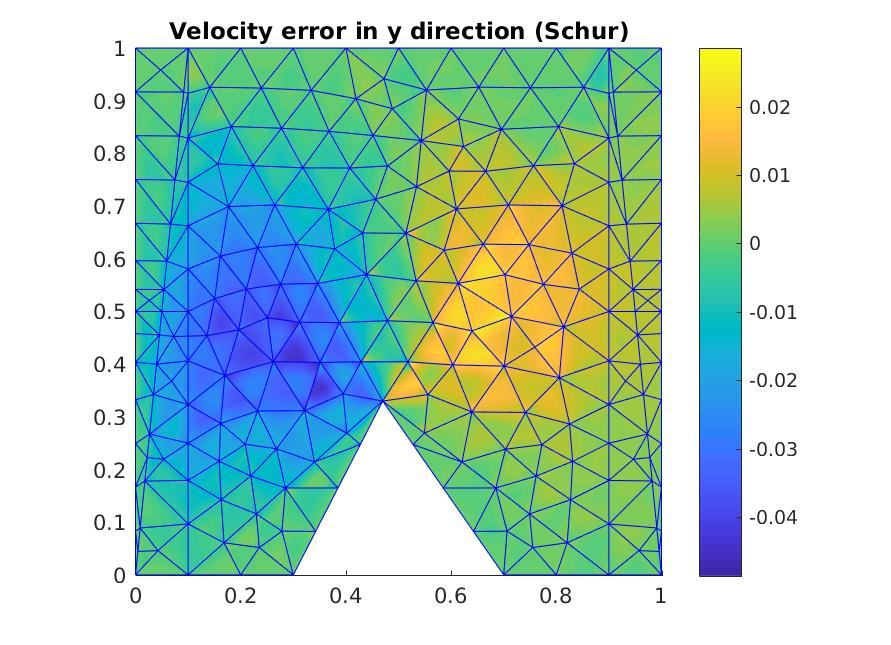
\includegraphics[width=\linewidth]{velocity_error_2_at_47_33.jpg}
\caption{$y-$component of Velocity absolute error $\overrightarrow{u}-\overrightarrow{u}_N$} \label{error_y_vel}
\end{subfigure}

\begin{subfigure}{0.31\textwidth}
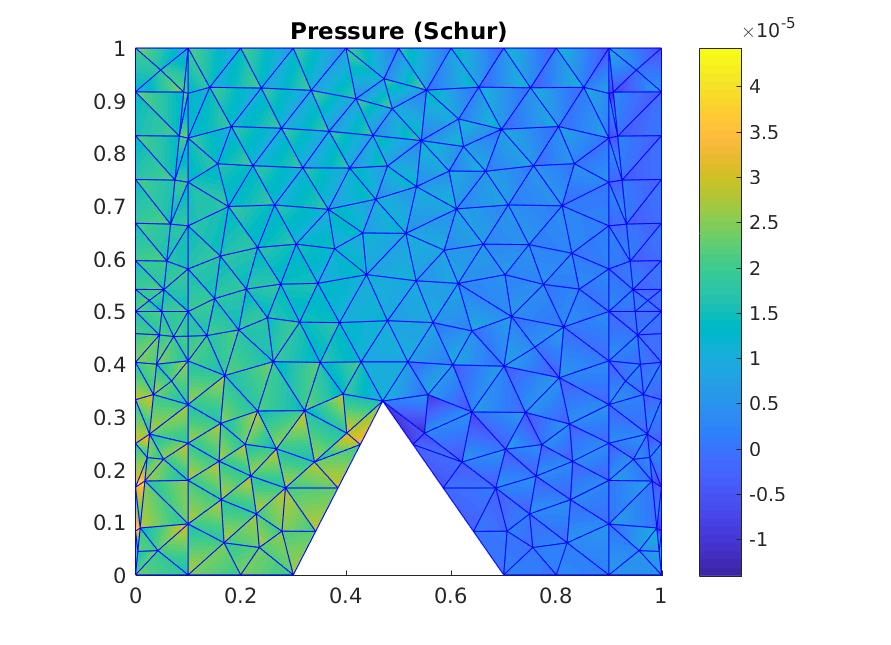
\includegraphics[width=\linewidth]{offline_pressure_at_47_33.jpg}
\caption{Pressure DG solution} \label{pre_dg}
\end{subfigure}\hspace*{\fill}
\begin{subfigure}{0.31\textwidth}
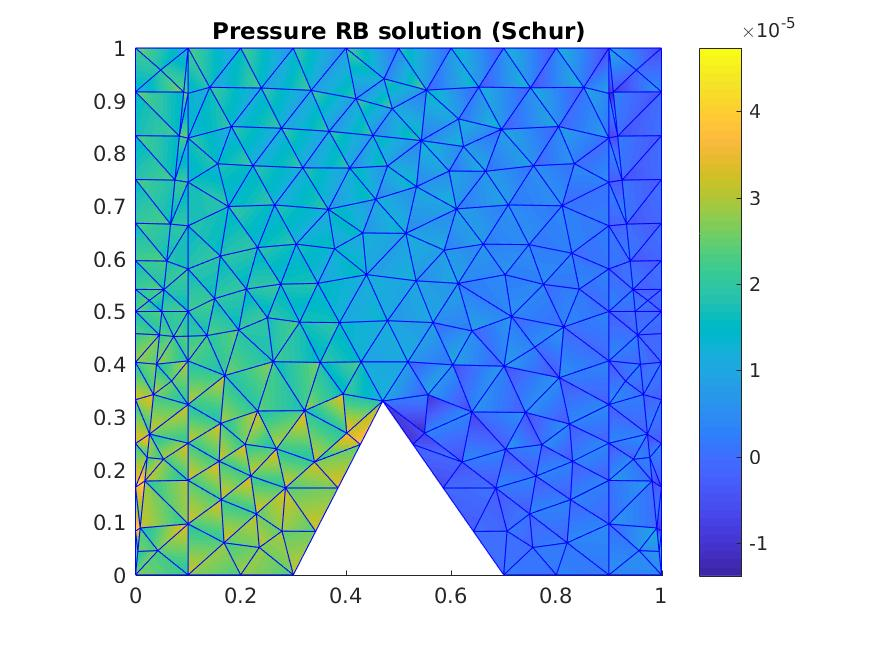
\includegraphics[width=\linewidth]{online_pressure_at_47_33.jpg}
\caption{Pressure RB solution} \label{pre_rb}
\end{subfigure}
\begin{subfigure}{0.31\textwidth}
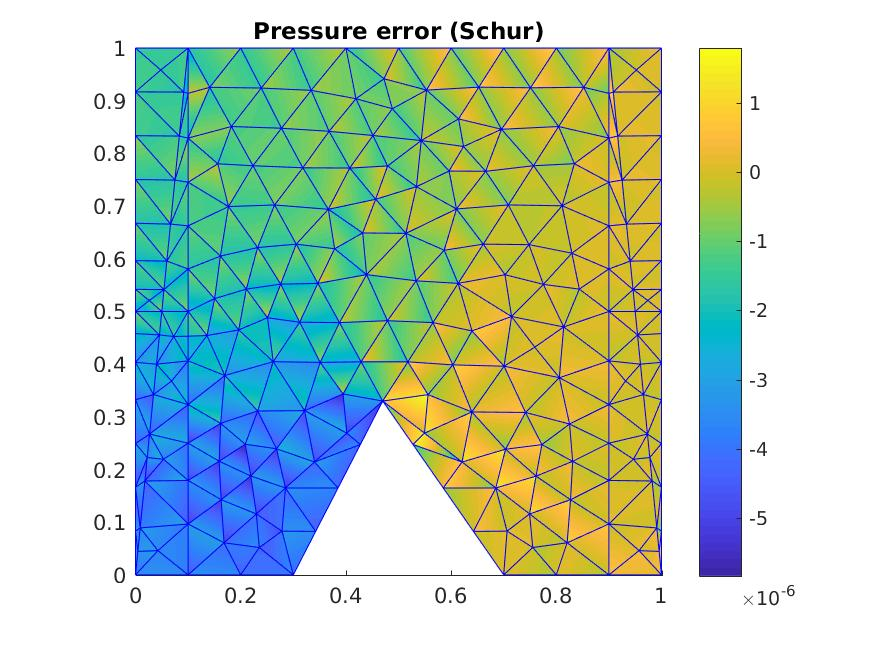
\includegraphics[width=\linewidth]{pressure_error_at_47_33.jpg}
\caption{Pressure absolute error $p-p_N$} \label{pre_error}
\end{subfigure}
\caption{DG and RB solution $[\mu_x \ \mu_y] = [0.47 \ 0.33]$} 
\label{dg_rb_solution_47_33}
\end{figure}

\begin{figure}
\begin{subfigure}{0.48\textwidth}
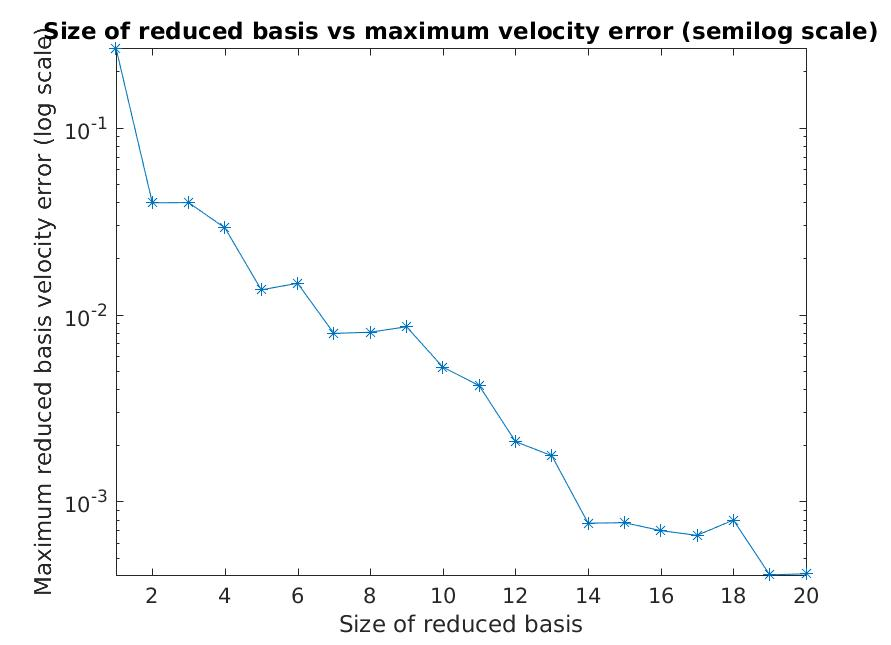
\includegraphics[width=\linewidth]{size_vs_maximum_reduced_basis_velocity_error_semilog.jpg}
\caption{Size of reduced basis space vs. Maximum relative error in velocity with inner product induced by $\bm{M}_v$} \label{error_vs_basis_velocity}
\end{subfigure}\hspace*{\fill}
\begin{subfigure}{0.48\textwidth}
\includegraphics[width=\linewidth]{size_vs_maximum_reduced_basis_pressure_error_semilog.jpg}
\caption{Size of reduced basis space vs. Maximum relative error in pressure with inner product induced by $\bm{M}_p$} \label{error_vs_basis_pressure}
\end{subfigure}
  \caption{Size of reduced basis vs Maximum relative error} 
\label{error_vs_basis}
\end{figure}

\begin{figure}
\begin{subfigure}{0.48\textwidth}
\includegraphics[width=\linewidth]{size_vs_online_simulation_time_semilog.jpg}
\caption{Size of reduced basis vs Online simulation time (semilog scale)} \label{online_simulation_time_vs_basis}
\end{subfigure}\hspace*{\fill}
\begin{subfigure}{0.48\textwidth}
\includegraphics[width=\linewidth]{size_vs_reduced_basis_semilog.jpg}
\caption{Size of reduced basis vs Speed up (semilog scale)} \label{time_vs_speedup}
\end{subfigure}
\caption{Size of reduced basis for velocity vs Online computational time} 
\label{basis_vs_time}
\end{figure}

\bibliographystyle{spbasic.bst}
\bibliography{references.tex}
\input{authorsample.bbl}
\end{document}

\end{document}

\end{document}



\end{document}
